%% fig_escape.tex   (generated by make_more.py; do not edit by hand)
%% The eight positions a secant construction can occupy, as the vertices of a cube.
\documentclass[tikz,border=8pt]{standalone}
\usepackage{amsmath,amssymb}
\usetikzlibrary{arrows.meta,calc}
%% palette.tex -- shared colour definitions for the figures
\definecolor{PInk}{RGB}{26,32,44}
\definecolor{PBlue}{RGB}{37,82,139}
\definecolor{PTeal}{RGB}{23,127,125}
\definecolor{POchre}{RGB}{193,138,44}
\definecolor{PClay}{RGB}{178,74,58}
\definecolor{PSlate}{RGB}{108,122,137}
\definecolor{PViolet}{RGB}{110,86,150}
\definecolor{WBlue}{RGB}{223,234,246}
\definecolor{WTeal}{RGB}{220,238,236}
\definecolor{WOchre}{RGB}{250,240,218}
\definecolor{WClay}{RGB}{247,229,224}
\definecolor{WSlate}{RGB}{238,241,244}
\definecolor{PMag}{RGB}{158,58,110}
\definecolor{PGrass}{RGB}{62,124,66}
\definecolor{PAmber}{RGB}{214,112,38}
\definecolor{PIndigo}{RGB}{58,64,140}
\definecolor{PRule}{RGB}{176,186,197}

%% shared macros so the standalone figures match the paper
\providecommand{\QQ}{\mathbb{Q}}
\providecommand{\ZZ}{\mathbb{Z}}
\providecommand{\RR}{\mathbb{R}}
\providecommand{\CC}{\mathbb{C}}
\providecommand{\PP}{\mathbb{P}}
\providecommand{\Kx}{K^{\times}}
\providecommand{\HW}{W}
\providecommand{\Nm}{\mathrm{N}}
\providecommand{\Hdg}{\mathrm{Hdg}}
\providecommand{\NS}{\mathrm{NS}}
\providecommand{\cA}{\mathcal{A}}
\providecommand{\cD}{\mathcal{D}}
\providecommand{\cF}{\mathcal{F}}
\providecommand{\cP}{\mathcal{P}}
\providecommand{\cO}{\mathcal{O}}
\providecommand{\cQ}{\mathcal{Q}}
\providecommand{\bbar}[1]{\overline{#1}}
\providecommand{\ch}{\operatorname{ch}}
\providecommand{\End}{\mathrm{End}}

\begin{document}
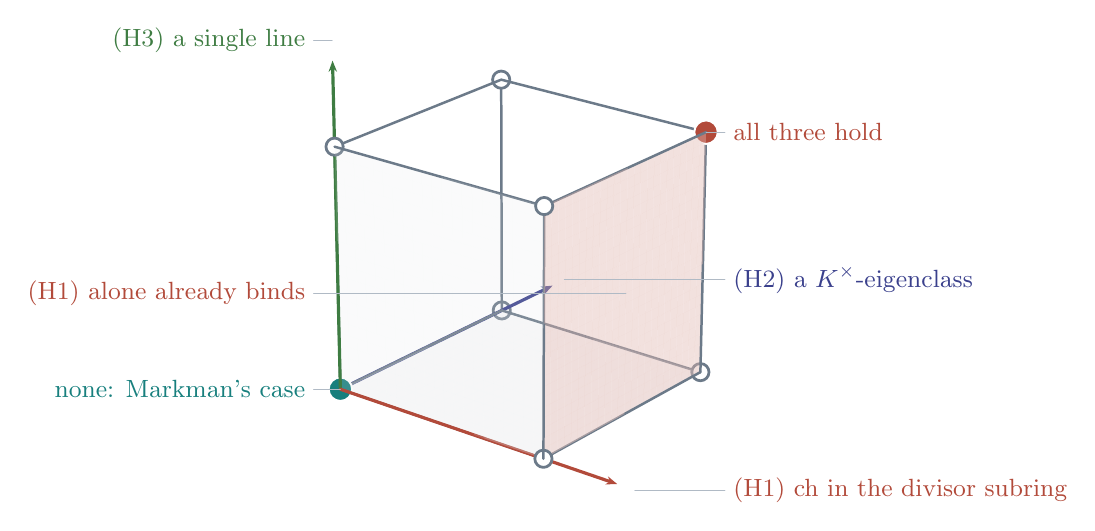
\begin{tikzpicture}[x=1cm,y=1cm,line join=round,line cap=round,
  font=\small,text=PInk]
  \node[circle,fill=white,draw=PSlate,line width=1.0pt,inner sep=2.2pt] at (-0.2504,-0.6164) {};
  \path[draw=none,fill opacity=0.16,fill=PSlate!20!white] (-0.3427,-0.6615) -- (-0.2276,-0.6974) -- (-0.1354,-0.6522) -- (-0.2504,-0.6164) -- cycle;
  \path[draw=none,fill opacity=0.16,fill=PSlate!20!white] (-0.2276,-0.6974) -- (-0.1121,-0.7335) -- (-0.0200,-0.6880) -- (-0.1354,-0.6522) -- cycle;
  \path[draw=none,fill opacity=0.16,fill=PSlate!20!white] (-0.4355,-0.7068) -- (-0.3203,-0.7429) -- (-0.2276,-0.6974) -- (-0.3427,-0.6615) -- cycle;
  \path[draw=none,fill opacity=0.16,fill=PSlate!20!white] (-0.1121,-0.7335) -- (0.0040,-0.7697) -- (0.0960,-0.7241) -- (-0.0200,-0.6880) -- cycle;
  \path[draw=none,fill opacity=0.16,fill=PSlate!20!white] (-0.3203,-0.7429) -- (-0.2047,-0.7792) -- (-0.1121,-0.7335) -- (-0.2276,-0.6974) -- cycle;
  \path[draw=none,fill opacity=0.16,fill=PSlate!20!white] (-0.5288,-0.7524) -- (-0.4136,-0.7887) -- (-0.3203,-0.7429) -- (-0.4355,-0.7068) -- cycle;
  \path[draw=none,fill opacity=0.16,fill=PSlate!20!white] (0.0040,-0.7697) -- (0.1206,-0.8061) -- (0.2124,-0.7603) -- (0.0960,-0.7241) -- cycle;
  \path[draw=none,fill opacity=0.16,fill=PSlate!20!white] (-0.2047,-0.7792) -- (-0.0885,-0.8156) -- (0.0040,-0.7697) -- (-0.1121,-0.7335) -- cycle;
  \path[draw=none,fill opacity=0.16,fill=PSlate!20!white] (-0.4136,-0.7887) -- (-0.2978,-0.8252) -- (-0.2047,-0.7792) -- (-0.3203,-0.7429) -- cycle;
  \path[draw=none,fill opacity=0.16,fill=PSlate!20!white] (-0.6227,-0.7982) -- (-0.5073,-0.8347) -- (-0.4136,-0.7887) -- (-0.5288,-0.7524) -- cycle;
  \path[draw=none,fill opacity=0.16,fill=PSlate!20!white] (0.1206,-0.8061) -- (0.2376,-0.8427) -- (0.3294,-0.7966) -- (0.2124,-0.7603) -- cycle;
  \path[draw=none,fill opacity=0.16,fill=PSlate!20!white] (-0.0885,-0.8156) -- (0.0282,-0.8522) -- (0.1206,-0.8061) -- (0.0040,-0.7697) -- cycle;
  \path[draw=none,fill opacity=0.16,fill=PSlate!20!white] (-0.2978,-0.8252) -- (-0.1815,-0.8618) -- (-0.0885,-0.8156) -- (-0.2047,-0.7792) -- cycle;
  \path[draw=none,fill opacity=0.16,fill=PSlate!20!white] (-0.5073,-0.8347) -- (-0.3914,-0.8714) -- (-0.2978,-0.8252) -- (-0.4136,-0.7887) -- cycle;
  \path[draw=none,fill opacity=0.16,fill=PSlate!20!white] (0.2376,-0.8427) -- (0.3552,-0.8794) -- (0.4468,-0.8331) -- (0.3294,-0.7966) -- cycle;
  \path[draw=none,fill opacity=0.16,fill=PSlate!20!white] (-0.7170,-0.8442) -- (-0.6015,-0.8810) -- (-0.5073,-0.8347) -- (-0.6227,-0.7982) -- cycle;
  \path[draw=none,fill opacity=0.16,fill=PSlate!20!white] (0.0282,-0.8522) -- (0.1454,-0.8890) -- (0.2376,-0.8427) -- (0.1206,-0.8061) -- cycle;
  \path[draw=none,fill opacity=0.16,fill=PSlate!20!white] (-0.1815,-0.8618) -- (-0.0647,-0.8986) -- (0.0282,-0.8522) -- (-0.0885,-0.8156) -- cycle;
  \draw[PSlate,line width=0.9pt] (-0.2504,-0.6164) -- (-0.2579,2.3141);
  \path[draw=none,fill opacity=0.16,fill=PSlate!20!white] (-0.3914,-0.8714) -- (-0.2750,-0.9082) -- (-0.1815,-0.8618) -- (-0.2978,-0.8252) -- cycle;
  \path[draw=none,fill opacity=0.16,fill=PSlate!20!white] (0.3552,-0.8794) -- (0.4733,-0.9162) -- (0.5648,-0.8698) -- (0.4468,-0.8331) -- cycle;
  \path[draw=none,fill opacity=0.16,fill=PSlate!20!white] (-0.6015,-0.8810) -- (-0.4855,-0.9178) -- (-0.3914,-0.8714) -- (-0.5073,-0.8347) -- cycle;
  \path[draw=none,fill opacity=0.16,fill=PSlate!20!white] (0.1454,-0.8890) -- (0.2631,-0.9259) -- (0.3552,-0.8794) -- (0.2376,-0.8427) -- cycle;
  \path[draw=none,fill opacity=0.16,fill=PSlate!20!white] (-0.8119,-0.8906) -- (-0.6963,-0.9275) -- (-0.6015,-0.8810) -- (-0.7170,-0.8442) -- cycle;
  \path[draw=none,fill opacity=0.16,fill=PSlate!20!white] (-0.0647,-0.8986) -- (0.0527,-0.9355) -- (0.1454,-0.8890) -- (0.0282,-0.8522) -- cycle;
  \path[draw=none,fill opacity=0.16,fill=PSlate!20!white] (-0.2750,-0.9082) -- (-0.1580,-0.9452) -- (-0.0647,-0.8986) -- (-0.1815,-0.8618) -- cycle;
  \path[draw=none,fill opacity=0.16,fill=PSlate!20!white] (0.4733,-0.9162) -- (0.5919,-0.9532) -- (0.6833,-0.9066) -- (0.5648,-0.8698) -- cycle;
  \path[draw=none,fill opacity=0.16,fill=PSlate!20!white] (-0.4855,-0.9178) -- (-0.3690,-0.9549) -- (-0.2750,-0.9082) -- (-0.3914,-0.8714) -- cycle;
  \path[draw=none,fill opacity=0.16,fill=PSlate!20!white] (0.2631,-0.9259) -- (0.3813,-0.9629) -- (0.4733,-0.9162) -- (0.3552,-0.8794) -- cycle;
  \path[draw=none,fill opacity=0.16,fill=PSlate!20!white] (-0.6963,-0.9275) -- (-0.5802,-0.9645) -- (-0.4855,-0.9178) -- (-0.6015,-0.8810) -- cycle;
  \path[draw=none,fill opacity=0.16,fill=PSlate!20!white] (0.0527,-0.9355) -- (0.1705,-0.9726) -- (0.2631,-0.9259) -- (0.1454,-0.8890) -- cycle;
  \path[draw=none,fill opacity=0.16,fill=PSlate!20!white] (-0.9073,-0.9371) -- (-0.7916,-0.9742) -- (-0.6963,-0.9275) -- (-0.8119,-0.8906) -- cycle;
  \draw[PIndigo,line width=1.15pt,-{Stealth[length=4pt]}] (-2.3001,-1.6170) -- (0.3946,-0.3016);
  \path[draw=none,fill opacity=0.16,fill=PSlate!20!white] (-0.1580,-0.9452) -- (-0.0406,-0.9823) -- (0.0527,-0.9355) -- (-0.0647,-0.8986) -- cycle;
  \path[draw=none,fill opacity=0.16,fill=PSlate!20!white] (0.5919,-0.9532) -- (0.7111,-0.9904) -- (0.8023,-0.9436) -- (0.6833,-0.9066) -- cycle;
  \path[draw=none,fill opacity=0.16,fill=PSlate!20!white] (-0.3690,-0.9549) -- (-0.2519,-0.9920) -- (-0.1580,-0.9452) -- (-0.2750,-0.9082) -- cycle;
  \path[draw=none,fill opacity=0.16,fill=PSlate!20!white] (0.3813,-0.9629) -- (0.5001,-1.0001) -- (0.5919,-0.9532) -- (0.4733,-0.9162) -- cycle;
  \path[draw=none,fill opacity=0.16,fill=PSlate!20!white] (-0.5802,-0.9645) -- (-0.4635,-1.0018) -- (-0.3690,-0.9549) -- (-0.4855,-0.9178) -- cycle;
  \path[draw=none,fill opacity=0.16,fill=PSlate!20!white] (0.1705,-0.9726) -- (0.2888,-1.0099) -- (0.3813,-0.9629) -- (0.2631,-0.9259) -- cycle;
  \path[draw=none,fill opacity=0.16,fill=PSlate!20!white] (-0.7916,-0.9742) -- (-0.6753,-1.0115) -- (-0.5802,-0.9645) -- (-0.6963,-0.9275) -- cycle;
  \path[draw=none,fill opacity=0.16,fill=PSlate!20!white] (-0.0406,-0.9823) -- (0.0773,-1.0196) -- (0.1705,-0.9726) -- (0.0527,-0.9355) -- cycle;
  \path[draw=none,fill opacity=0.16,fill=PSlate!20!white] (-1.0032,-0.9839) -- (-0.8874,-1.0213) -- (-0.7916,-0.9742) -- (-0.9073,-0.9371) -- cycle;
  \path[draw=none,fill opacity=0.16,fill=PSlate!20!white] (0.7111,-0.9904) -- (0.8307,-1.0278) -- (0.9218,-0.9807) -- (0.8023,-0.9436) -- cycle;
  \path[draw=none,fill opacity=0.16,fill=PSlate!20!white] (-0.2519,-0.9920) -- (-0.1344,-1.0294) -- (-0.0406,-0.9823) -- (-0.1580,-0.9452) -- cycle;
  \path[draw=none,fill opacity=0.16,fill=PSlate!20!white] (0.5001,-1.0001) -- (0.6193,-1.0375) -- (0.7111,-0.9904) -- (0.5919,-0.9532) -- cycle;
  \path[draw=none,fill opacity=0.16,fill=PSlate!20!white] (-0.4635,-1.0018) -- (-0.3464,-1.0392) -- (-0.2519,-0.9920) -- (-0.3690,-0.9549) -- cycle;
  \draw[PSlate,line width=0.9pt] (-0.2504,-0.6164) -- (2.2719,-1.4003);
  \path[draw=none,fill opacity=0.16,fill=PSlate!20!white] (0.2888,-1.0099) -- (0.4077,-1.0473) -- (0.5001,-1.0001) -- (0.3813,-0.9629) -- cycle;
  \path[draw=none,fill opacity=0.16,fill=PSlate!20!white] (-0.6753,-1.0115) -- (-0.5586,-1.0490) -- (-0.4635,-1.0018) -- (-0.5802,-0.9645) -- cycle;
  \path[draw=none,fill opacity=0.16,fill=PSlate!20!white] (0.0773,-1.0196) -- (0.1958,-1.0571) -- (0.2888,-1.0099) -- (0.1705,-0.9726) -- cycle;
  \path[draw=none,fill opacity=0.16,fill=PSlate!20!white] (-0.8874,-1.0213) -- (-0.7710,-1.0587) -- (-0.6753,-1.0115) -- (-0.7916,-0.9742) -- cycle;
  \path[draw=none,fill opacity=0.16,fill=PSlate!20!white] (0.8307,-1.0278) -- (0.9509,-1.0653) -- (1.0419,-1.0180) -- (0.9218,-0.9807) -- cycle;
  \path[draw=none,fill opacity=0.16,fill=PSlate!20!white] (-0.1344,-1.0294) -- (-0.0163,-1.0669) -- (0.0773,-1.0196) -- (-0.0406,-0.9823) -- cycle;
  \path[draw=none,fill opacity=0.16,fill=PSlate!20!white] (-1.0997,-1.0310) -- (-0.9837,-1.0686) -- (-0.8874,-1.0213) -- (-1.0032,-0.9839) -- cycle;
  \path[draw=none,fill opacity=0.16,fill=PSlate!20!white] (0.6193,-1.0375) -- (0.7391,-1.0751) -- (0.8307,-1.0278) -- (0.7111,-0.9904) -- cycle;
  \path[draw=none,fill opacity=0.16,fill=PSlate!20!white] (-0.3464,-1.0392) -- (-0.2287,-1.0767) -- (-0.1344,-1.0294) -- (-0.2519,-0.9920) -- cycle;
  \path[draw=none,fill opacity=0.16,fill=PSlate!20!white] (0.4077,-1.0473) -- (0.5271,-1.0849) -- (0.6193,-1.0375) -- (0.5001,-1.0001) -- cycle;
  \path[draw=none,fill opacity=0.16,fill=PSlate!20!white] (-0.5586,-1.0490) -- (-0.4413,-1.0866) -- (-0.3464,-1.0392) -- (-0.4635,-1.0018) -- cycle;
  \path[draw=none,fill opacity=0.16,fill=PSlate!20!white] (0.1958,-1.0571) -- (0.3148,-1.0948) -- (0.4077,-1.0473) -- (0.2888,-1.0099) -- cycle;
  \path[draw=none,fill opacity=0.16,fill=PSlate!20!white] (-0.7710,-1.0587) -- (-0.6542,-1.0964) -- (-0.5586,-1.0490) -- (-0.6753,-1.0115) -- cycle;
  \path[draw=none,fill opacity=0.16,fill=PSlate!20!white] (0.9509,-1.0653) -- (1.0716,-1.1030) -- (1.1624,-1.0555) -- (1.0419,-1.0180) -- cycle;
  \path[draw=none,fill opacity=0.16,fill=PSlate!20!white] (-0.0163,-1.0669) -- (0.1023,-1.1046) -- (0.1958,-1.0571) -- (0.0773,-1.0196) -- cycle;
  \path[draw=none,fill opacity=0.16,fill=PSlate!20!white] (-0.9837,-1.0686) -- (-0.8672,-1.1062) -- (-0.7710,-1.0587) -- (-0.8874,-1.0213) -- cycle;
  \path[draw=none,fill opacity=0.16,fill=PSlate!20!white] (0.7391,-1.0751) -- (0.8594,-1.1128) -- (0.9509,-1.0653) -- (0.8307,-1.0278) -- cycle;
  \path[draw=none,fill opacity=0.16,fill=PSlate!20!white] (-0.2287,-1.0767) -- (-0.1105,-1.1145) -- (-0.0163,-1.0669) -- (-0.1344,-1.0294) -- cycle;
  \path[draw=none,fill opacity=0.16,fill=PSlate!20!white] (-1.1967,-1.0784) -- (-1.0806,-1.1161) -- (-0.9837,-1.0686) -- (-1.0997,-1.0310) -- cycle;
  \path[draw=none,fill opacity=0.16,fill=PSlate!20!white] (0.5271,-1.0849) -- (0.6470,-1.1227) -- (0.7391,-1.0751) -- (0.6193,-1.0375) -- cycle;
  \path[draw=none,fill opacity=0.16,fill=PSlate!20!white] (-0.4413,-1.0866) -- (-0.3235,-1.1243) -- (-0.2287,-1.0767) -- (-0.3464,-1.0392) -- cycle;
  \path[draw=none,fill opacity=0.16,fill=PSlate!20!white] (0.3148,-1.0948) -- (0.4343,-1.1326) -- (0.5271,-1.0849) -- (0.4077,-1.0473) -- cycle;
  \path[draw=none,fill opacity=0.16,fill=PSlate!20!white] (-0.6542,-1.0964) -- (-0.5368,-1.1342) -- (-0.4413,-1.0866) -- (-0.5586,-1.0490) -- cycle;
  \path[draw=none,fill opacity=0.16,fill=PSlate!20!white] (1.0716,-1.1030) -- (1.1928,-1.1408) -- (1.2835,-1.0931) -- (1.1624,-1.0555) -- cycle;
  \path[draw=none,fill opacity=0.16,fill=PSlate!20!white] (0.1023,-1.1046) -- (0.2214,-1.1425) -- (0.3148,-1.0948) -- (0.1958,-1.0571) -- cycle;
  \path[draw=none,fill opacity=0.16,fill=PSlate!20!white] (-0.8672,-1.1062) -- (-0.7503,-1.1441) -- (-0.6542,-1.0964) -- (-0.7710,-1.0587) -- cycle;
  \draw[PSlate,line width=0.9pt] (-2.3001,-1.6170) -- (-0.2504,-0.6164);
  \path[draw=none,fill opacity=0.16,fill=PSlate!20!white] (0.8594,-1.1128) -- (0.9802,-1.1507) -- (1.0716,-1.1030) -- (0.9509,-1.0653) -- cycle;
  \path[draw=none,fill opacity=0.16,fill=PSlate!20!white] (-0.1105,-1.1145) -- (0.0082,-1.1524) -- (0.1023,-1.1046) -- (-0.0163,-1.0669) -- cycle;
  \path[draw=none,fill opacity=0.16,fill=PSlate!20!white] (-1.0806,-1.1161) -- (-0.9640,-1.1540) -- (-0.8672,-1.1062) -- (-0.9837,-1.0686) -- cycle;
  \path[draw=none,fill opacity=0.16,fill=PSlate!20!white] (0.6470,-1.1227) -- (0.7674,-1.1606) -- (0.8594,-1.1128) -- (0.7391,-1.0751) -- cycle;
  \path[draw=none,fill opacity=0.16,fill=PSlate!20!white] (-0.3235,-1.1243) -- (-0.2052,-1.1623) -- (-0.1105,-1.1145) -- (-0.2287,-1.0767) -- cycle;
  \node[circle,fill=white,draw=PSlate,line width=1.0pt,inner sep=2.2pt] at (-0.2579,2.3141) {};
  \path[draw=none,fill opacity=0.16,fill=PSlate!20!white] (-1.2942,-1.1260) -- (-1.1780,-1.1639) -- (-1.0806,-1.1161) -- (-1.1967,-1.0784) -- cycle;
  \path[draw=none,fill opacity=0.16,fill=PSlate!20!white] (0.4343,-1.1326) -- (0.5543,-1.1705) -- (0.6470,-1.1227) -- (0.5271,-1.0849) -- cycle;
  \path[draw=none,fill opacity=0.16,fill=PSlate!20!white] (-0.5368,-1.1342) -- (-0.4189,-1.1722) -- (-0.3235,-1.1243) -- (-0.4413,-1.0866) -- cycle;
  \path[draw=none,fill opacity=0.16,fill=PSlate!20!white] (1.1928,-1.1408) -- (1.3146,-1.1788) -- (1.4052,-1.1309) -- (1.2835,-1.0931) -- cycle;
  \path[draw=none,fill opacity=0.16,fill=PSlate!20!white] (0.2214,-1.1425) -- (0.3410,-1.1805) -- (0.4343,-1.1326) -- (0.3148,-1.0948) -- cycle;
  \path[draw=none,fill opacity=0.16,fill=PSlate!20!white] (-0.7503,-1.1441) -- (-0.6328,-1.1821) -- (-0.5368,-1.1342) -- (-0.6542,-1.0964) -- cycle;
  \path[draw=none,fill opacity=0.16,fill=PSlate!20!white] (0.9802,-1.1507) -- (1.1016,-1.1888) -- (1.1928,-1.1408) -- (1.0716,-1.1030) -- cycle;
  \path[draw=none,fill opacity=0.16,fill=PSlate!20!white] (0.0082,-1.1524) -- (0.1274,-1.1904) -- (0.2214,-1.1425) -- (0.1023,-1.1046) -- cycle;
  \path[draw=none,fill opacity=0.16,fill=PSlate!20!white] (-0.9640,-1.1540) -- (-0.8469,-1.1921) -- (-0.7503,-1.1441) -- (-0.8672,-1.1062) -- cycle;
  \path[draw=none,fill opacity=0.16,fill=PSlate!20!white] (0.7674,-1.1606) -- (0.8884,-1.1987) -- (0.9802,-1.1507) -- (0.8594,-1.1128) -- cycle;
  \path[draw=none,fill opacity=0.16,fill=PSlate!20!white] (-0.2052,-1.1623) -- (-0.0864,-1.2004) -- (0.0082,-1.1524) -- (-0.1105,-1.1145) -- cycle;
  \path[draw=none,fill opacity=0.16,fill=PSlate!20!white] (-1.1780,-1.1639) -- (-1.0613,-1.2020) -- (-0.9640,-1.1540) -- (-1.0806,-1.1161) -- cycle;
  \path[draw=none,fill opacity=0.16,fill=PSlate!20!white] (0.5543,-1.1705) -- (0.6749,-1.2087) -- (0.7674,-1.1606) -- (0.6470,-1.1227) -- cycle;
  \path[draw=none,fill opacity=0.16,fill=PSlate!20!white] (-0.4189,-1.1722) -- (-0.3004,-1.2103) -- (-0.2052,-1.1623) -- (-0.3235,-1.1243) -- cycle;
  \path[draw=none,fill opacity=0.16,fill=PSlate!20!white] (-1.3922,-1.1738) -- (-1.2760,-1.2120) -- (-1.1780,-1.1639) -- (-1.2942,-1.1260) -- cycle;
  \path[draw=none,fill opacity=0.16,fill=PSlate!20!white] (1.3146,-1.1788) -- (1.4369,-1.2170) -- (1.5273,-1.1689) -- (1.4052,-1.1309) -- cycle;
  \path[draw=none,fill opacity=0.16,fill=PSlate!20!white] (0.3410,-1.1805) -- (0.4612,-1.2187) -- (0.5543,-1.1705) -- (0.4343,-1.1326) -- cycle;
  \path[draw=none,fill opacity=0.16,fill=PSlate!20!white] (-0.6328,-1.1821) -- (-0.5147,-1.2203) -- (-0.4189,-1.1722) -- (-0.5368,-1.1342) -- cycle;
  \path[draw=none,fill opacity=0.16,fill=PSlate!20!white] (1.1016,-1.1888) -- (1.2235,-1.2270) -- (1.3146,-1.1788) -- (1.1928,-1.1408) -- cycle;
  \path[draw=none,fill opacity=0.16,fill=PSlate!20!white] (0.1274,-1.1904) -- (0.2472,-1.2286) -- (0.3410,-1.1805) -- (0.2214,-1.1425) -- cycle;
  \path[draw=none,fill opacity=0.16,fill=PSlate!20!white] (-0.8469,-1.1921) -- (-0.7293,-1.2303) -- (-0.6328,-1.1821) -- (-0.7503,-1.1441) -- cycle;
  \path[draw=none,fill opacity=0.16,fill=PSlate!20!white] (0.8884,-1.1987) -- (1.0099,-1.2370) -- (1.1016,-1.1888) -- (0.9802,-1.1507) -- cycle;
  \path[draw=none,fill opacity=0.16,fill=PSlate!20!white] (-0.0864,-1.2004) -- (0.0330,-1.2386) -- (0.1274,-1.1904) -- (0.0082,-1.1524) -- cycle;
  \path[draw=none,fill opacity=0.16,fill=PSlate!20!white] (-1.0613,-1.2020) -- (-0.9441,-1.2403) -- (-0.8469,-1.1921) -- (-0.9640,-1.1540) -- cycle;
  \path[draw=none,fill opacity=0.16,fill=PSlate!20!white] (0.6749,-1.2087) -- (0.7960,-1.2470) -- (0.8884,-1.1987) -- (0.7674,-1.1606) -- cycle;
  \path[draw=none,fill opacity=0.16,fill=PSlate!20!white] (-0.3004,-1.2103) -- (-0.1815,-1.2487) -- (-0.0864,-1.2004) -- (-0.2052,-1.1623) -- cycle;
  \path[draw=none,fill opacity=0.16,fill=PSlate!20!white] (-1.2760,-1.2120) -- (-1.1592,-1.2503) -- (-1.0613,-1.2020) -- (-1.1780,-1.1639) -- cycle;
  \path[draw=none,fill opacity=0.16,fill=PSlate!20!white] (1.4369,-1.2170) -- (1.5598,-1.2553) -- (1.6500,-1.2070) -- (1.5273,-1.1689) -- cycle;
  \path[draw=none,fill opacity=0.16,fill=PSlate!20!white] (0.4612,-1.2187) -- (0.5819,-1.2570) -- (0.6749,-1.2087) -- (0.5543,-1.1705) -- cycle;
  \path[draw=none,fill opacity=0.16,fill=PSlate!20!white] (-0.5147,-1.2203) -- (-0.3962,-1.2587) -- (-0.3004,-1.2103) -- (-0.4189,-1.1722) -- cycle;
  \path[draw=none,fill opacity=0.16,fill=PSlate!20!white] (-1.4909,-1.2220) -- (-1.3745,-1.2604) -- (-1.2760,-1.2120) -- (-1.3922,-1.1738) -- cycle;
  \path[draw=none,fill opacity=0.16,fill=PSlate!20!white] (1.2235,-1.2270) -- (1.3460,-1.2654) -- (1.4369,-1.2170) -- (1.3146,-1.1788) -- cycle;
  \path[draw=none,fill opacity=0.16,fill=PSlate!20!white] (0.2472,-1.2286) -- (0.3675,-1.2670) -- (0.4612,-1.2187) -- (0.3410,-1.1805) -- cycle;
  \path[draw=none,fill opacity=0.16,fill=PSlate!20!white] (-0.7293,-1.2303) -- (-0.6112,-1.2687) -- (-0.5147,-1.2203) -- (-0.6328,-1.1821) -- cycle;
  \path[draw=none,fill opacity=0.16,fill=PSlate!20!white] (1.0099,-1.2370) -- (1.1319,-1.2754) -- (1.2235,-1.2270) -- (1.1016,-1.1888) -- cycle;
  \path[draw=none,fill opacity=0.16,fill=PSlate!20!white] (0.0330,-1.2386) -- (0.1529,-1.2771) -- (0.2472,-1.2286) -- (0.1274,-1.1904) -- cycle;
  \path[draw=none,fill opacity=0.16,fill=PSlate!20!white] (-0.9441,-1.2403) -- (-0.8264,-1.2788) -- (-0.7293,-1.2303) -- (-0.8469,-1.1921) -- cycle;
  \path[draw=none,fill opacity=0.16,fill=PSlate!20!white] (0.7960,-1.2470) -- (0.9176,-1.2855) -- (1.0099,-1.2370) -- (0.8884,-1.1987) -- cycle;
  \path[draw=none,fill opacity=0.16,fill=PSlate!20!white] (-0.1815,-1.2487) -- (-0.0620,-1.2871) -- (0.0330,-1.2386) -- (-0.0864,-1.2004) -- cycle;
  \path[draw=none,fill opacity=0.16,fill=PSlate!20!white] (-1.1592,-1.2503) -- (-1.0419,-1.2888) -- (-0.9441,-1.2403) -- (-1.0613,-1.2020) -- cycle;
  \path[draw=none,fill opacity=0.16,fill=PSlate!20!white] (1.5598,-1.2553) -- (1.6832,-1.2939) -- (1.7733,-1.2453) -- (1.6500,-1.2070) -- cycle;
  \path[draw=none,fill opacity=0.16,fill=PSlate!20!white] (0.5819,-1.2570) -- (0.7031,-1.2955) -- (0.7960,-1.2470) -- (0.6749,-1.2087) -- cycle;
  \path[draw=none,fill opacity=0.16,fill=PSlate!20!white] (-0.3962,-1.2587) -- (-0.2771,-1.2972) -- (-0.1815,-1.2487) -- (-0.3004,-1.2103) -- cycle;
  \path[draw=none,fill opacity=0.16,fill=PSlate!20!white] (-1.3745,-1.2604) -- (-1.2576,-1.2989) -- (-1.1592,-1.2503) -- (-1.2760,-1.2120) -- cycle;
  \path[draw=none,fill opacity=0.16,fill=PSlate!20!white] (1.3460,-1.2654) -- (1.4690,-1.3039) -- (1.5598,-1.2553) -- (1.4369,-1.2170) -- cycle;
  \path[draw=none,fill opacity=0.16,fill=PSlate!20!white] (0.3675,-1.2670) -- (0.4883,-1.3056) -- (0.5819,-1.2570) -- (0.4612,-1.2187) -- cycle;
  \path[draw=none,fill opacity=0.16,fill=PSlate!20!white] (-0.6112,-1.2687) -- (-0.4925,-1.3073) -- (-0.3962,-1.2587) -- (-0.5147,-1.2203) -- cycle;
  \path[draw=none,fill opacity=0.16,fill=PSlate!20!white] (-1.5900,-1.2704) -- (-1.4735,-1.3090) -- (-1.3745,-1.2604) -- (-1.4909,-1.2220) -- cycle;
  \path[draw=none,fill opacity=0.16,fill=PSlate!20!white] (1.1319,-1.2754) -- (1.2545,-1.3140) -- (1.3460,-1.2654) -- (1.2235,-1.2270) -- cycle;
  \path[draw=none,fill opacity=0.16,fill=PSlate!20!white] (0.1529,-1.2771) -- (0.2733,-1.3157) -- (0.3675,-1.2670) -- (0.2472,-1.2286) -- cycle;
  \path[draw=none,fill opacity=0.16,fill=PSlate!20!white] (-0.8264,-1.2788) -- (-0.7081,-1.3174) -- (-0.6112,-1.2687) -- (-0.7293,-1.2303) -- cycle;
  \path[draw=none,fill opacity=0.16,fill=PSlate!20!white] (0.9176,-1.2855) -- (1.0398,-1.3241) -- (1.1319,-1.2754) -- (1.0099,-1.2370) -- cycle;
  \path[draw=none,fill opacity=0.16,fill=PSlate!20!white] (-0.0620,-1.2871) -- (0.0580,-1.3258) -- (0.1529,-1.2771) -- (0.0330,-1.2386) -- cycle;
  \path[draw=none,fill opacity=0.16,fill=PSlate!20!white] (-1.0419,-1.2888) -- (-0.9240,-1.3275) -- (-0.8264,-1.2788) -- (-0.9441,-1.2403) -- cycle;
  \path[draw=none,fill opacity=0.16,fill=PSlate!20!white] (1.6832,-1.2939) -- (1.8071,-1.3325) -- (1.8971,-1.2838) -- (1.7733,-1.2453) -- cycle;
  \path[draw=none,fill opacity=0.16,fill=PSlate!20!white] (0.7031,-1.2955) -- (0.8249,-1.3342) -- (0.9176,-1.2855) -- (0.7960,-1.2470) -- cycle;
  \path[draw=none,fill opacity=0.16,fill=PSlate!20!white] (-0.2771,-1.2972) -- (-0.1575,-1.3359) -- (-0.0620,-1.2871) -- (-0.1815,-1.2487) -- cycle;
  \path[draw=none,fill opacity=0.16,fill=PSlate!20!white] (-1.2576,-1.2989) -- (-1.1401,-1.3376) -- (-1.0419,-1.2888) -- (-1.1592,-1.2503) -- cycle;
  \path[draw=none,fill opacity=0.16,fill=PSlate!20!white] (1.4690,-1.3039) -- (1.5925,-1.3427) -- (1.6832,-1.2939) -- (1.5598,-1.2553) -- cycle;
  \path[draw=none,fill opacity=0.16,fill=PSlate!20!white] (0.4883,-1.3056) -- (0.6097,-1.3444) -- (0.7031,-1.2955) -- (0.5819,-1.2570) -- cycle;
  \path[draw=none,fill opacity=0.16,fill=PSlate!20!white] (-0.4925,-1.3073) -- (-0.3733,-1.3460) -- (-0.2771,-1.2972) -- (-0.3962,-1.2587) -- cycle;
  \path[draw=none,fill opacity=0.16,fill=PSlate!20!white] (-1.4735,-1.3090) -- (-1.3565,-1.3477) -- (-1.2576,-1.2989) -- (-1.3745,-1.2604) -- cycle;
  \path[draw=none,fill opacity=0.16,fill=PSlate!20!white] (1.2545,-1.3140) -- (1.3777,-1.3528) -- (1.4690,-1.3039) -- (1.3460,-1.2654) -- cycle;
  \path[draw=none,fill opacity=0.16,fill=PSlate!20!white] (0.2733,-1.3157) -- (0.3942,-1.3545) -- (0.4883,-1.3056) -- (0.3675,-1.2670) -- cycle;
  \path[draw=none,fill opacity=0.16,fill=PSlate!20!white] (-0.7081,-1.3174) -- (-0.5894,-1.3562) -- (-0.4925,-1.3073) -- (-0.6112,-1.2687) -- cycle;
  \path[draw=none,fill opacity=0.16,fill=PSlate!20!white] (-1.6897,-1.3191) -- (-1.5732,-1.3579) -- (-1.4735,-1.3090) -- (-1.5900,-1.2704) -- cycle;
  \path[draw=none,fill opacity=0.16,fill=PSlate!20!white] (1.0398,-1.3241) -- (1.1626,-1.3630) -- (1.2545,-1.3140) -- (1.1319,-1.2754) -- cycle;
  \path[draw=none,fill opacity=0.16,fill=PSlate!20!white] (0.0580,-1.3258) -- (0.1786,-1.3646) -- (0.2733,-1.3157) -- (0.1529,-1.2771) -- cycle;
  \path[draw=none,fill opacity=0.16,fill=PSlate!20!white] (-0.9240,-1.3275) -- (-0.8056,-1.3663) -- (-0.7081,-1.3174) -- (-0.8264,-1.2788) -- cycle;
  \path[draw=none,fill opacity=0.16,fill=PSlate!20!white] (1.8071,-1.3325) -- (1.9316,-1.3714) -- (2.0215,-1.3224) -- (1.8971,-1.2838) -- cycle;
  \path[draw=none,fill opacity=0.16,fill=PSlate!20!white] (0.8249,-1.3342) -- (0.9472,-1.3731) -- (1.0398,-1.3241) -- (0.9176,-1.2855) -- cycle;
  \path[draw=none,fill opacity=0.16,fill=PSlate!20!white] (-0.1575,-1.3359) -- (-0.0374,-1.3748) -- (0.0580,-1.3258) -- (-0.0620,-1.2871) -- cycle;
  \path[draw=none,fill opacity=0.16,fill=PSlate!20!white] (-1.1401,-1.3376) -- (-1.0222,-1.3765) -- (-0.9240,-1.3275) -- (-1.0419,-1.2888) -- cycle;
  \path[draw=none,fill opacity=0.16,fill=PSlate!20!white] (1.5925,-1.3427) -- (1.7166,-1.3816) -- (1.8071,-1.3325) -- (1.6832,-1.2939) -- cycle;
  \path[draw=none,fill opacity=0.16,fill=PSlate!20!white] (0.6097,-1.3444) -- (0.7316,-1.3833) -- (0.8249,-1.3342) -- (0.7031,-1.2955) -- cycle;
  \path[draw=none,fill opacity=0.16,fill=PSlate!20!white] (-0.3733,-1.3460) -- (-0.2536,-1.3850) -- (-0.1575,-1.3359) -- (-0.2771,-1.2972) -- cycle;
  \path[draw=none,fill opacity=0.16,fill=PSlate!20!white] (-1.3565,-1.3477) -- (-1.2390,-1.3867) -- (-1.1401,-1.3376) -- (-1.2576,-1.2989) -- cycle;
  \path[draw=none,fill opacity=0.16,fill=PSlate!20!white] (1.3777,-1.3528) -- (1.5014,-1.3918) -- (1.5925,-1.3427) -- (1.4690,-1.3039) -- cycle;
  \path[draw=none,fill opacity=0.16,fill=PSlate!20!white] (0.3942,-1.3545) -- (0.5158,-1.3935) -- (0.6097,-1.3444) -- (0.4883,-1.3056) -- cycle;
  \path[draw=none,fill opacity=0.16,fill=PSlate!20!white] (-0.5894,-1.3562) -- (-0.4700,-1.3952) -- (-0.3733,-1.3460) -- (-0.4925,-1.3073) -- cycle;
  \path[draw=none,fill opacity=0.16,fill=PSlate!20!white] (-1.5732,-1.3579) -- (-1.4560,-1.3969) -- (-1.3565,-1.3477) -- (-1.4735,-1.3090) -- cycle;
  \path[draw=none,fill opacity=0.16,fill=PSlate!20!white] (1.1626,-1.3630) -- (1.2858,-1.4020) -- (1.3777,-1.3528) -- (1.2545,-1.3140) -- cycle;
  \path[draw=none,fill opacity=0.16,fill=PSlate!20!white] (0.1786,-1.3646) -- (0.2996,-1.4037) -- (0.3942,-1.3545) -- (0.2733,-1.3157) -- cycle;
  \path[draw=none,fill opacity=0.16,fill=PSlate!20!white] (-0.8056,-1.3663) -- (-0.6867,-1.4054) -- (-0.5894,-1.3562) -- (-0.7081,-1.3174) -- cycle;
  \path[draw=none,fill opacity=0.16,fill=PSlate!20!white] (-1.7900,-1.3680) -- (-1.6733,-1.4071) -- (-1.5732,-1.3579) -- (-1.6897,-1.3191) -- cycle;
  \path[draw=none,fill opacity=0.16,fill=PSlate!20!white] (1.9316,-1.3714) -- (2.0567,-1.4105) -- (2.1464,-1.3613) -- (2.0215,-1.3224) -- cycle;
  \path[draw=none,fill opacity=0.16,fill=PSlate!20!white] (0.9472,-1.3731) -- (1.0701,-1.4122) -- (1.1626,-1.3630) -- (1.0398,-1.3241) -- cycle;
  \path[draw=none,fill opacity=0.16,fill=PSlate!20!white] (-0.0374,-1.3748) -- (0.0833,-1.4139) -- (0.1786,-1.3646) -- (0.0580,-1.3258) -- cycle;
  \path[draw=none,fill opacity=0.16,fill=PSlate!20!white] (-1.0222,-1.3765) -- (-0.9037,-1.4156) -- (-0.8056,-1.3663) -- (-0.9240,-1.3275) -- cycle;
  \path[draw=none,fill opacity=0.16,fill=PSlate!20!white] (1.7166,-1.3816) -- (1.8413,-1.4207) -- (1.9316,-1.3714) -- (1.8071,-1.3325) -- cycle;
  \path[draw=none,fill opacity=0.16,fill=PSlate!20!white] (0.7316,-1.3833) -- (0.8541,-1.4224) -- (0.9472,-1.3731) -- (0.8249,-1.3342) -- cycle;
  \path[draw=none,fill opacity=0.16,fill=PSlate!20!white] (-0.2536,-1.3850) -- (-0.1333,-1.4241) -- (-0.0374,-1.3748) -- (-0.1575,-1.3359) -- cycle;
  \path[draw=none,fill opacity=0.16,fill=PSlate!20!white] (-1.2390,-1.3867) -- (-1.1209,-1.4258) -- (-1.0222,-1.3765) -- (-1.1401,-1.3376) -- cycle;
  \path[draw=none,fill opacity=0.16,fill=PSlate!20!white] (1.5014,-1.3918) -- (1.6256,-1.4309) -- (1.7166,-1.3816) -- (1.5925,-1.3427) -- cycle;
  \path[draw=none,fill opacity=0.16,fill=PSlate!20!white] (0.5158,-1.3935) -- (0.6378,-1.4326) -- (0.7316,-1.3833) -- (0.6097,-1.3444) -- cycle;
  \path[draw=none,fill opacity=0.16,fill=PSlate!20!white] (-0.4700,-1.3952) -- (-0.3502,-1.4343) -- (-0.2536,-1.3850) -- (-0.3733,-1.3460) -- cycle;
  \path[draw=none,fill opacity=0.16,fill=PSlate!20!white] (-1.4560,-1.3969) -- (-1.3384,-1.4360) -- (-1.2390,-1.3867) -- (-1.3565,-1.3477) -- cycle;
  \path[draw=none,fill opacity=0.16,fill=PSlate!20!white] (1.2858,-1.4020) -- (1.4097,-1.4411) -- (1.5014,-1.3918) -- (1.3777,-1.3528) -- cycle;
  \path[draw=none,fill opacity=0.16,fill=PSlate!20!white] (0.2996,-1.4037) -- (0.4213,-1.4428) -- (0.5158,-1.3935) -- (0.3942,-1.3545) -- cycle;
  \path[draw=none,fill opacity=0.16,fill=PSlate!20!white] (-0.6867,-1.4054) -- (-0.5673,-1.4445) -- (-0.4700,-1.3952) -- (-0.5894,-1.3562) -- cycle;
  \node[circle,fill=white,draw=PSlate,line width=1.0pt,inner sep=2.2pt] at (2.2719,-1.4003) {};
  \path[draw=none,fill opacity=0.16,fill=PSlate!20!white] (-1.6733,-1.4071) -- (-1.5561,-1.4462) -- (-1.4560,-1.3969) -- (-1.5732,-1.3579) -- cycle;
  \path[draw=none,fill opacity=0.16,fill=PSlate!20!white] (2.0567,-1.4105) -- (2.1823,-1.4497) -- (2.2719,-1.4003) -- (2.1464,-1.3613) -- cycle;
  \path[draw=none,fill opacity=0.16,fill=PSlate!20!white] (1.0701,-1.4122) -- (1.1935,-1.4514) -- (1.2858,-1.4020) -- (1.1626,-1.3630) -- cycle;
  \path[draw=none,fill opacity=0.16,fill=PSlate!20!white] (0.0833,-1.4139) -- (0.2045,-1.4531) -- (0.2996,-1.4037) -- (0.1786,-1.3646) -- cycle;
  \path[draw=none,fill opacity=0.16,fill=PSlate!20!white] (-0.9037,-1.4156) -- (-0.7847,-1.4548) -- (-0.6867,-1.4054) -- (-0.8056,-1.3663) -- cycle;
  \path[draw=none,fill opacity=0.16,fill=PSlate!20!white] (-1.8909,-1.4173) -- (-1.7741,-1.4565) -- (-1.6733,-1.4071) -- (-1.7900,-1.3680) -- cycle;
  \path[draw=none,fill opacity=0.16,fill=PSlate!20!white] (1.8413,-1.4207) -- (1.9665,-1.4599) -- (2.0567,-1.4105) -- (1.9316,-1.3714) -- cycle;
  \path[draw=none,fill opacity=0.16,fill=PSlate!20!white] (0.8541,-1.4224) -- (0.9771,-1.4616) -- (1.0701,-1.4122) -- (0.9472,-1.3731) -- cycle;
  \path[draw=none,fill opacity=0.16,fill=PSlate!20!white] (-0.1333,-1.4241) -- (-0.0125,-1.4633) -- (0.0833,-1.4139) -- (-0.0374,-1.3748) -- cycle;
  \path[draw=none,fill opacity=0.16,fill=PSlate!20!white] (-1.1209,-1.4258) -- (-1.0023,-1.4651) -- (-0.9037,-1.4156) -- (-1.0222,-1.3765) -- cycle;
  \path[draw=none,fill opacity=0.16,fill=PSlate!20!white] (1.6256,-1.4309) -- (1.7504,-1.4702) -- (1.8413,-1.4207) -- (1.7166,-1.3816) -- cycle;
  \path[draw=none,fill opacity=0.16,fill=PSlate!20!white] (0.6378,-1.4326) -- (0.7604,-1.4719) -- (0.8541,-1.4224) -- (0.7316,-1.3833) -- cycle;
  \path[draw=none,fill opacity=0.16,fill=PSlate!20!white] (-0.3502,-1.4343) -- (-0.2298,-1.4736) -- (-0.1333,-1.4241) -- (-0.2536,-1.3850) -- cycle;
  \path[draw=none,fill opacity=0.16,fill=PSlate!20!white] (-1.3384,-1.4360) -- (-1.2202,-1.4753) -- (-1.1209,-1.4258) -- (-1.2390,-1.3867) -- cycle;
  \path[draw=none,fill opacity=0.42,fill=PClay!40!white] (2.1935,-1.4435) -- (2.2719,-1.4003) -- (2.2748,-1.2770) -- (2.1963,-1.3200) -- cycle;
  \path[draw=none,fill opacity=0.16,fill=PSlate!20!white] (1.4097,-1.4411) -- (1.5341,-1.4805) -- (1.6256,-1.4309) -- (1.5014,-1.3918) -- cycle;
  \path[draw=none,fill opacity=0.16,fill=PSlate!20!white] (0.4213,-1.4428) -- (0.5435,-1.4822) -- (0.6378,-1.4326) -- (0.5158,-1.3935) -- cycle;
  \path[draw=none,fill opacity=0.16,fill=PSlate!20!white] (-0.5673,-1.4445) -- (-0.4474,-1.4839) -- (-0.3502,-1.4343) -- (-0.4700,-1.3952) -- cycle;
  \path[draw=none,fill opacity=0.16,fill=PSlate!20!white] (-1.5561,-1.4462) -- (-1.4384,-1.4856) -- (-1.3384,-1.4360) -- (-1.4560,-1.3969) -- cycle;
  \path[draw=none,fill opacity=0.16,fill=PSlate!20!white] (1.1935,-1.4514) -- (1.3175,-1.4908) -- (1.4097,-1.4411) -- (1.2858,-1.4020) -- cycle;
  \path[draw=none,fill opacity=0.16,fill=PSlate!20!white] (0.2045,-1.4531) -- (0.3263,-1.4925) -- (0.4213,-1.4428) -- (0.2996,-1.4037) -- cycle;
  \path[draw=none,fill opacity=0.16,fill=PSlate!20!white] (-0.7847,-1.4548) -- (-0.6651,-1.4942) -- (-0.5673,-1.4445) -- (-0.6867,-1.4054) -- cycle;
  \path[draw=none,fill opacity=0.16,fill=PSlate!20!white] (-1.7741,-1.4565) -- (-1.6568,-1.4959) -- (-1.5561,-1.4462) -- (-1.6733,-1.4071) -- cycle;
  \path[draw=none,fill opacity=0.16,fill=PSlate!20!white] (1.9665,-1.4599) -- (2.0923,-1.4994) -- (2.1823,-1.4497) -- (2.0567,-1.4105) -- cycle;
  \path[draw=none,fill opacity=0.42,fill=PClay!40!white] (2.1963,-1.3200) -- (2.2748,-1.2770) -- (2.2777,-1.1534) -- (2.1992,-1.1961) -- cycle;
  \path[draw=none,fill opacity=0.16,fill=PSlate!20!white] (0.9771,-1.4616) -- (1.1006,-1.5011) -- (1.1935,-1.4514) -- (1.0701,-1.4122) -- cycle;
  \path[draw=none,fill opacity=0.16,fill=PSlate!20!white] (-0.0125,-1.4633) -- (0.1088,-1.5028) -- (0.2045,-1.4531) -- (0.0833,-1.4139) -- cycle;
  \path[draw=none,fill opacity=0.16,fill=PSlate!20!white] (-1.0023,-1.4651) -- (-0.8832,-1.5045) -- (-0.7847,-1.4548) -- (-0.9037,-1.4156) -- cycle;
  \path[draw=none,fill opacity=0.16,fill=PSlate!20!white] (-1.9923,-1.4668) -- (-1.8754,-1.5062) -- (-1.7741,-1.4565) -- (-1.8909,-1.4173) -- cycle;
  \path[draw=none,fill opacity=0.16,fill=PSlate!20!white] (1.7504,-1.4702) -- (1.8758,-1.5097) -- (1.9665,-1.4599) -- (1.8413,-1.4207) -- cycle;
  \path[draw=none,fill opacity=0.16,fill=PSlate!20!white] (0.7604,-1.4719) -- (0.8835,-1.5114) -- (0.9771,-1.4616) -- (0.8541,-1.4224) -- cycle;
  \path[draw=none,fill opacity=0.16,fill=PSlate!20!white] (-0.2298,-1.4736) -- (-0.1089,-1.5131) -- (-0.0125,-1.4633) -- (-0.1333,-1.4241) -- cycle;
  \path[draw=none,fill opacity=0.16,fill=PSlate!20!white] (-1.2202,-1.4753) -- (-1.1015,-1.5148) -- (-1.0023,-1.4651) -- (-1.1209,-1.4258) -- cycle;
  \path[draw=none,fill opacity=0.16,fill=PSlate!20!white] (1.5341,-1.4805) -- (1.6590,-1.5200) -- (1.7504,-1.4702) -- (1.6256,-1.4309) -- cycle;
  \path[draw=none,fill opacity=0.42,fill=PClay!40!white] (2.1148,-1.4869) -- (2.1935,-1.4435) -- (2.1963,-1.3200) -- (2.1175,-1.3631) -- cycle;
  \path[draw=none,fill opacity=0.16,fill=PSlate!20!white] (0.5435,-1.4822) -- (0.6662,-1.5217) -- (0.7604,-1.4719) -- (0.6378,-1.4326) -- cycle;
  \path[draw=none,fill opacity=0.42,fill=PClay!40!white] (2.1992,-1.1961) -- (2.2777,-1.1534) -- (2.2806,-1.0295) -- (2.2020,-1.0720) -- cycle;
  \path[draw=none,fill opacity=0.16,fill=PSlate!20!white] (-0.4474,-1.4839) -- (-0.3268,-1.5235) -- (-0.2298,-1.4736) -- (-0.3502,-1.4343) -- cycle;
  \path[draw=none,fill opacity=0.16,fill=PSlate!20!white] (-1.4384,-1.4856) -- (-1.3201,-1.5252) -- (-1.2202,-1.4753) -- (-1.3384,-1.4360) -- cycle;
  \path[draw=none,fill opacity=0.16,fill=PSlate!20!white] (1.3175,-1.4908) -- (1.4420,-1.5303) -- (1.5341,-1.4805) -- (1.4097,-1.4411) -- cycle;
  \path[draw=none,fill opacity=0.16,fill=PSlate!20!white] (0.3263,-1.4925) -- (0.4486,-1.5321) -- (0.5435,-1.4822) -- (0.4213,-1.4428) -- cycle;
  \path[draw=none,fill opacity=0.16,fill=PSlate!20!white] (-0.6651,-1.4942) -- (-0.5451,-1.5338) -- (-0.4474,-1.4839) -- (-0.5673,-1.4445) -- cycle;
  \path[draw=none,fill opacity=0.16,fill=PSlate!20!white] (-1.6568,-1.4959) -- (-1.5389,-1.5355) -- (-1.4384,-1.4856) -- (-1.5561,-1.4462) -- cycle;
  \path[draw=none,fill opacity=0.16,fill=PSlate!20!white] (1.1006,-1.5011) -- (1.2248,-1.5407) -- (1.3175,-1.4908) -- (1.1935,-1.4514) -- cycle;
  \path[draw=none,fill opacity=0.16,fill=PSlate!20!white] (0.1088,-1.5028) -- (0.2307,-1.5424) -- (0.3263,-1.4925) -- (0.2045,-1.4531) -- cycle;
  \path[draw=none,fill opacity=0.42,fill=PClay!40!white] (2.1175,-1.3631) -- (2.1963,-1.3200) -- (2.1992,-1.1961) -- (2.1203,-1.2391) -- cycle;
  \path[draw=none,fill opacity=0.16,fill=PSlate!20!white] (-0.8832,-1.5045) -- (-0.7635,-1.5442) -- (-0.6651,-1.4942) -- (-0.7847,-1.4548) -- cycle;
  \path[draw=none,fill opacity=0.42,fill=PClay!40!white] (2.2020,-1.0720) -- (2.2806,-1.0295) -- (2.2835,-0.9053) -- (2.2048,-0.9475) -- cycle;
  \path[draw=none,fill opacity=0.16,fill=PSlate!20!white] (-1.8754,-1.5062) -- (-1.7580,-1.5459) -- (-1.6568,-1.4959) -- (-1.7741,-1.4565) -- cycle;
  \path[draw=none,fill opacity=0.16,fill=PSlate!20!white] (1.8758,-1.5097) -- (2.0017,-1.5493) -- (2.0923,-1.4994) -- (1.9665,-1.4599) -- cycle;
  \path[draw=none,fill opacity=0.16,fill=PSlate!20!white] (0.8835,-1.5114) -- (1.0072,-1.5511) -- (1.1006,-1.5011) -- (0.9771,-1.4616) -- cycle;
  \path[draw=none,fill opacity=0.16,fill=PSlate!20!white] (-0.1089,-1.5131) -- (0.0126,-1.5528) -- (0.1088,-1.5028) -- (-0.0125,-1.4633) -- cycle;
  \path[draw=none,fill opacity=0.16,fill=PSlate!20!white] (-1.1015,-1.5148) -- (-0.9823,-1.5545) -- (-0.8832,-1.5045) -- (-1.0023,-1.4651) -- cycle;
  \path[draw=none,fill opacity=0.16,fill=PSlate!20!white] (-2.0943,-1.5166) -- (-1.9773,-1.5563) -- (-1.8754,-1.5062) -- (-1.9923,-1.4668) -- cycle;
  \path[draw=none,fill opacity=0.16,fill=PSlate!20!white] (1.6590,-1.5200) -- (1.7845,-1.5597) -- (1.8758,-1.5097) -- (1.7504,-1.4702) -- cycle;
  \path[draw=none,fill opacity=0.16,fill=PSlate!20!white] (0.6662,-1.5217) -- (0.7895,-1.5614) -- (0.8835,-1.5114) -- (0.7604,-1.4719) -- cycle;
  \path[draw=none,fill opacity=0.16,fill=PSlate!20!white] (-0.3268,-1.5235) -- (-0.2058,-1.5632) -- (-0.1089,-1.5131) -- (-0.2298,-1.4736) -- cycle;
  \path[draw=none,fill opacity=0.42,fill=PClay!40!white] (2.0357,-1.5306) -- (2.1148,-1.4869) -- (2.1175,-1.3631) -- (2.0384,-1.4066) -- cycle;
  \path[draw=none,fill opacity=0.16,fill=PSlate!20!white] (-1.3201,-1.5252) -- (-1.2012,-1.5649) -- (-1.1015,-1.5148) -- (-1.2202,-1.4753) -- cycle;
  \path[draw=none,fill opacity=0.42,fill=PClay!40!white] (2.1203,-1.2391) -- (2.1992,-1.1961) -- (2.2020,-1.0720) -- (2.1230,-1.1147) -- cycle;
  \path[draw=none,fill opacity=0.42,fill=PClay!40!white] (2.2048,-0.9475) -- (2.2835,-0.9053) -- (2.2865,-0.7808) -- (2.2077,-0.8227) -- cycle;
  \path[draw=none,fill opacity=0.16,fill=PSlate!20!white] (1.4420,-1.5303) -- (1.5671,-1.5701) -- (1.6590,-1.5200) -- (1.5341,-1.4805) -- cycle;
  \draw[PSlate,line width=0.9pt] (-0.2579,2.3141) -- (2.3437,1.6477);
  \path[draw=none,fill opacity=0.16,fill=PSlate!20!white] (0.4486,-1.5321) -- (0.5714,-1.5718) -- (0.6662,-1.5217) -- (0.5435,-1.4822) -- cycle;
  \path[draw=none,fill opacity=0.16,fill=PSlate!20!white] (-0.5451,-1.5338) -- (-0.4244,-1.5736) -- (-0.3268,-1.5235) -- (-0.4474,-1.4839) -- cycle;
  \path[draw=none,fill opacity=0.16,fill=PSlate!20!white] (-1.5389,-1.5355) -- (-1.4205,-1.5753) -- (-1.3201,-1.5252) -- (-1.4384,-1.4856) -- cycle;
  \path[draw=none,fill opacity=0.16,fill=PSlate!20!white] (1.2248,-1.5407) -- (1.3494,-1.5805) -- (1.4420,-1.5303) -- (1.3175,-1.4908) -- cycle;
  \path[draw=none,fill opacity=0.16,fill=PSlate!20!white] (0.2307,-1.5424) -- (0.3532,-1.5822) -- (0.4486,-1.5321) -- (0.3263,-1.4925) -- cycle;
  \path[draw=none,fill opacity=0.16,fill=PSlate!20!white] (-0.7635,-1.5442) -- (-0.6433,-1.5840) -- (-0.5451,-1.5338) -- (-0.6651,-1.4942) -- cycle;
  \path[draw=none,fill opacity=0.16,fill=PSlate!20!white] (-1.7580,-1.5459) -- (-1.6400,-1.5857) -- (-1.5389,-1.5355) -- (-1.6568,-1.4959) -- cycle;
  \path[draw=none,fill opacity=0.42,fill=PClay!40!white] (2.0384,-1.4066) -- (2.1175,-1.3631) -- (2.1203,-1.2391) -- (2.0410,-1.2822) -- cycle;
  \path[draw=none,fill opacity=0.42,fill=PClay!40!white] (2.1230,-1.1147) -- (2.2020,-1.0720) -- (2.2048,-0.9475) -- (2.1257,-0.9899) -- cycle;
  \path[draw=none,fill opacity=0.42,fill=PClay!40!white] (2.2077,-0.8227) -- (2.2865,-0.7808) -- (2.2894,-0.6559) -- (2.2105,-0.6976) -- cycle;
  \path[draw=none,fill opacity=0.16,fill=PSlate!20!white] (1.0072,-1.5511) -- (1.1315,-1.5909) -- (1.2248,-1.5407) -- (1.1006,-1.5011) -- cycle;
  \path[draw=none,fill opacity=0.16,fill=PSlate!20!white] (0.0126,-1.5528) -- (0.1346,-1.5927) -- (0.2307,-1.5424) -- (0.1088,-1.5028) -- cycle;
  \path[draw=none,fill opacity=0.16,fill=PSlate!20!white] (-0.9823,-1.5545) -- (-0.8625,-1.5944) -- (-0.7635,-1.5442) -- (-0.8832,-1.5045) -- cycle;
  \path[draw=none,fill opacity=0.16,fill=PSlate!20!white] (-1.9773,-1.5563) -- (-1.8598,-1.5961) -- (-1.7580,-1.5459) -- (-1.8754,-1.5062) -- cycle;
  \path[draw=none,fill opacity=0.16,fill=PSlate!20!white] (1.7845,-1.5597) -- (1.9106,-1.5996) -- (2.0017,-1.5493) -- (1.8758,-1.5097) -- cycle;
  \path[draw=none,fill opacity=0.16,fill=PSlate!20!white] (0.7895,-1.5614) -- (0.9133,-1.6013) -- (1.0072,-1.5511) -- (0.8835,-1.5114) -- cycle;
  \path[draw=none,fill opacity=0.16,fill=PSlate!20!white] (-0.2058,-1.5632) -- (-0.0842,-1.6031) -- (0.0126,-1.5528) -- (-0.1089,-1.5131) -- cycle;
  \path[draw=none,fill opacity=0.16,fill=PSlate!20!white] (-1.2012,-1.5649) -- (-1.0819,-1.6048) -- (-0.9823,-1.5545) -- (-1.1015,-1.5148) -- cycle;
  \path[draw=none,fill opacity=0.16,fill=PSlate!20!white] (-2.1969,-1.5666) -- (-2.0798,-1.6066) -- (-1.9773,-1.5563) -- (-2.0943,-1.5166) -- cycle;
  \path[draw=none,fill opacity=0.42,fill=PClay!40!white] (1.9562,-1.5744) -- (2.0357,-1.5306) -- (2.0384,-1.4066) -- (1.9588,-1.4502) -- cycle;
  \path[draw=none,fill opacity=0.16,fill=PSlate!20!white] (1.5671,-1.5701) -- (1.6928,-1.6100) -- (1.7845,-1.5597) -- (1.6590,-1.5200) -- cycle;
  \path[draw=none,fill opacity=0.42,fill=PClay!40!white] (2.0410,-1.2822) -- (2.1203,-1.2391) -- (2.1230,-1.1147) -- (2.0436,-1.1576) -- cycle;
  \path[draw=none,fill opacity=0.16,fill=PSlate!20!white] (0.5714,-1.5718) -- (0.6949,-1.6118) -- (0.7895,-1.5614) -- (0.6662,-1.5217) -- cycle;
  \path[draw=none,fill opacity=0.42,fill=PClay!40!white] (2.1257,-0.9899) -- (2.2048,-0.9475) -- (2.2077,-0.8227) -- (2.1285,-0.8649) -- cycle;
  \path[draw=none,fill opacity=0.42,fill=PClay!40!white] (2.2105,-0.6976) -- (2.2894,-0.6559) -- (2.2924,-0.5308) -- (2.2134,-0.5722) -- cycle;
  \path[draw=none,fill opacity=0.16,fill=PSlate!20!white] (-0.4244,-1.5736) -- (-0.3032,-1.6135) -- (-0.2058,-1.5632) -- (-0.3268,-1.5235) -- cycle;
  \path[draw=none,fill opacity=0.16,fill=PSlate!20!white] (-1.4205,-1.5753) -- (-1.3016,-1.6153) -- (-1.2012,-1.5649) -- (-1.3201,-1.5252) -- cycle;
  \path[draw=none,fill opacity=0.16,fill=PSlate!20!white] (1.3494,-1.5805) -- (1.4747,-1.6205) -- (1.5671,-1.5701) -- (1.4420,-1.5303) -- cycle;
  \path[draw=none,fill opacity=0.16,fill=PSlate!20!white] (0.3532,-1.5822) -- (0.4762,-1.6222) -- (0.5714,-1.5718) -- (0.4486,-1.5321) -- cycle;
  \path[draw=none,fill opacity=0.16,fill=PSlate!20!white] (-0.6433,-1.5840) -- (-0.5226,-1.6240) -- (-0.4244,-1.5736) -- (-0.5451,-1.5338) -- cycle;
  \path[draw=none,fill opacity=0.16,fill=PSlate!20!white] (-1.6400,-1.5857) -- (-1.5215,-1.6257) -- (-1.4205,-1.5753) -- (-1.5389,-1.5355) -- cycle;
  \path[draw=none,fill opacity=0.16,fill=PSlate!20!white] (1.1315,-1.5909) -- (1.2563,-1.6309) -- (1.3494,-1.5805) -- (1.2248,-1.5407) -- cycle;
  \path[draw=none,fill opacity=0.42,fill=PClay!40!white] (1.9588,-1.4502) -- (2.0384,-1.4066) -- (2.0410,-1.2822) -- (1.9613,-1.3256) -- cycle;
  \path[draw=none,fill opacity=0.16,fill=PSlate!20!white] (0.1346,-1.5927) -- (0.2572,-1.6327) -- (0.3532,-1.5822) -- (0.2307,-1.5424) -- cycle;
  \path[draw=none,fill opacity=0.42,fill=PClay!40!white] (2.0436,-1.1576) -- (2.1230,-1.1147) -- (2.1257,-0.9899) -- (2.0463,-1.0326) -- cycle;
  \path[draw=none,fill opacity=0.16,fill=PSlate!20!white] (-0.8625,-1.5944) -- (-0.7421,-1.6344) -- (-0.6433,-1.5840) -- (-0.7635,-1.5442) -- cycle;
  \path[draw=none,fill opacity=0.42,fill=PClay!40!white] (2.1285,-0.8649) -- (2.2077,-0.8227) -- (2.2105,-0.6976) -- (2.1313,-0.7395) -- cycle;
  \path[draw=none,fill opacity=0.16,fill=PSlate!20!white] (-1.8598,-1.5961) -- (-1.7417,-1.6362) -- (-1.6400,-1.5857) -- (-1.7580,-1.5459) -- cycle;
  \path[draw=none,fill opacity=0.42,fill=PClay!40!white] (2.2134,-0.5722) -- (2.2924,-0.5308) -- (2.2953,-0.4053) -- (2.2162,-0.4464) -- cycle;
  \path[draw=none,fill opacity=0.16,fill=PSlate!20!white] (0.9133,-1.6013) -- (1.0377,-1.6414) -- (1.1315,-1.5909) -- (1.0072,-1.5511) -- cycle;
  \path[draw=none,fill opacity=0.16,fill=PSlate!20!white] (-0.0842,-1.6031) -- (0.0380,-1.6432) -- (0.1346,-1.5927) -- (0.0126,-1.5528) -- cycle;
  \path[draw=none,fill opacity=0.16,fill=PSlate!20!white] (-1.0819,-1.6048) -- (-0.9620,-1.6449) -- (-0.8625,-1.5944) -- (-0.9823,-1.5545) -- cycle;
  \path[draw=none,fill opacity=0.16,fill=PSlate!20!white] (-2.0798,-1.6066) -- (-1.9621,-1.6467) -- (-1.8598,-1.5961) -- (-1.9773,-1.5563) -- cycle;
  \path[draw=none,fill opacity=0.16,fill=PSlate!20!white] (1.6928,-1.6100) -- (1.8190,-1.6502) -- (1.9106,-1.5996) -- (1.7845,-1.5597) -- cycle;
  \path[draw=none,fill opacity=0.16,fill=PSlate!20!white] (0.6949,-1.6118) -- (0.8189,-1.6519) -- (0.9133,-1.6013) -- (0.7895,-1.5614) -- cycle;
  \path[draw=none,fill opacity=0.42,fill=PClay!40!white] (1.8763,-1.6185) -- (1.9562,-1.5744) -- (1.9588,-1.4502) -- (1.8788,-1.4940) -- cycle;
  \path[draw=none,fill opacity=0.16,fill=PSlate!20!white] (-0.3032,-1.6135) -- (-0.1815,-1.6537) -- (-0.0842,-1.6031) -- (-0.2058,-1.5632) -- cycle;
  \path[draw=none,fill opacity=0.42,fill=PClay!40!white] (1.9613,-1.3256) -- (2.0410,-1.2822) -- (2.0436,-1.1576) -- (1.9638,-1.2007) -- cycle;
  \path[draw=none,fill opacity=0.16,fill=PSlate!20!white] (-1.3016,-1.6153) -- (-1.1821,-1.6554) -- (-1.0819,-1.6048) -- (-1.2012,-1.5649) -- cycle;
  \path[draw=none,fill opacity=0.42,fill=PClay!40!white] (2.0463,-1.0326) -- (2.1257,-0.9899) -- (2.1285,-0.8649) -- (2.0489,-0.9073) -- cycle;
  \path[draw=none,fill opacity=0.16,fill=PSlate!20!white] (-2.3001,-1.6170) -- (-2.1829,-1.6572) -- (-2.0798,-1.6066) -- (-2.1969,-1.5666) -- cycle;
  \path[draw=none,fill opacity=0.42,fill=PClay!40!white] (2.1313,-0.7395) -- (2.2105,-0.6976) -- (2.2134,-0.5722) -- (2.1340,-0.6138) -- cycle;
  \path[draw=none,fill opacity=0.42,fill=PClay!40!white] (2.2162,-0.4464) -- (2.2953,-0.4053) -- (2.2983,-0.2794) -- (2.2191,-0.3204) -- cycle;
  \path[draw=none,fill opacity=0.16,fill=PSlate!20!white] (1.4747,-1.6205) -- (1.6005,-1.6607) -- (1.6928,-1.6100) -- (1.5671,-1.5701) -- cycle;
  \node[circle,fill=PTeal,draw=white,line width=0.7pt,inner sep=3.0pt] at (-2.3001,-1.6170) {};
  \path[draw=none,fill opacity=0.16,fill=PSlate!20!white] (0.4762,-1.6222) -- (0.5997,-1.6624) -- (0.6949,-1.6118) -- (0.5714,-1.5718) -- cycle;
  \path[draw=none,fill opacity=0.16,fill=PSlate!20!white] (-0.5226,-1.6240) -- (-0.4013,-1.6642) -- (-0.3032,-1.6135) -- (-0.4244,-1.5736) -- cycle;
  \path[draw=none,fill opacity=0.16,fill=PSlate!20!white] (-1.5215,-1.6257) -- (-1.4025,-1.6659) -- (-1.3016,-1.6153) -- (-1.4205,-1.5753) -- cycle;
  \path[draw=none,fill opacity=0.16,fill=PSlate!20!white] (1.2563,-1.6309) -- (1.3817,-1.6712) -- (1.4747,-1.6205) -- (1.3494,-1.5805) -- cycle;
  \path[draw=none,fill opacity=0.16,fill=PSlate!20!white] (0.2572,-1.6327) -- (0.3803,-1.6729) -- (0.4762,-1.6222) -- (0.3532,-1.5822) -- cycle;
  \path[draw=none,fill opacity=0.16,fill=PSlate!20!white] (-0.7421,-1.6344) -- (-0.6213,-1.6747) -- (-0.5226,-1.6240) -- (-0.6433,-1.5840) -- cycle;
  \path[draw=none,fill opacity=0.42,fill=PClay!40!white] (1.8788,-1.4940) -- (1.9588,-1.4502) -- (1.9613,-1.3256) -- (1.8812,-1.3692) -- cycle;
  \path[draw=none,fill opacity=0.16,fill=PSlate!20!white] (-1.7417,-1.6362) -- (-1.6231,-1.6764) -- (-1.5215,-1.6257) -- (-1.6400,-1.5857) -- cycle;
  \path[draw=none,fill opacity=0.42,fill=PClay!40!white] (1.9638,-1.2007) -- (2.0436,-1.1576) -- (2.0463,-1.0326) -- (1.9664,-1.0754) -- cycle;
  \path[draw=none,fill opacity=0.42,fill=PClay!40!white] (2.0489,-0.9073) -- (2.1285,-0.8649) -- (2.1313,-0.7395) -- (2.0516,-0.7817) -- cycle;
  \path[draw=none,fill opacity=0.42,fill=PClay!40!white] (2.1340,-0.6138) -- (2.2134,-0.5722) -- (2.2162,-0.4464) -- (2.1368,-0.4878) -- cycle;
  \draw[PSlate,line width=0.9pt] (-2.3738,1.4631) -- (-0.2579,2.3141);
  \path[draw=none,fill opacity=0.16,fill=PSlate!20!white] (1.0377,-1.6414) -- (1.1627,-1.6817) -- (1.2563,-1.6309) -- (1.1315,-1.5909) -- cycle;
  \path[draw=none,fill opacity=0.42,fill=PClay!40!white] (2.2191,-0.3204) -- (2.2983,-0.2794) -- (2.3013,-0.1533) -- (2.2220,-0.1939) -- cycle;
  \path[draw=none,fill opacity=0.16,fill=PSlate!20!white] (0.0380,-1.6432) -- (0.1607,-1.6834) -- (0.2572,-1.6327) -- (0.1346,-1.5927) -- cycle;
  \path[draw=none,fill opacity=0.16,fill=PSlate!20!white] (-0.9620,-1.6449) -- (-0.8415,-1.6852) -- (-0.7421,-1.6344) -- (-0.8625,-1.5944) -- cycle;
  \path[draw=none,fill opacity=0.16,fill=PSlate!20!white] (-1.9621,-1.6467) -- (-1.8440,-1.6869) -- (-1.7417,-1.6362) -- (-1.8598,-1.5961) -- cycle;
  \path[draw=none,fill opacity=0.16,fill=PSlate!20!white] (0.8189,-1.6519) -- (0.9434,-1.6922) -- (1.0377,-1.6414) -- (0.9133,-1.6013) -- cycle;
  \path[draw=none,fill opacity=0.16,fill=PSlate!20!white] (-0.1815,-1.6537) -- (-0.0592,-1.6940) -- (0.0380,-1.6432) -- (-0.0842,-1.6031) -- cycle;
  \path[draw=none,fill opacity=0.16,fill=PSlate!20!white] (-1.1821,-1.6554) -- (-1.0621,-1.6957) -- (-0.9620,-1.6449) -- (-1.0819,-1.6048) -- cycle;
  \path[draw=none,fill opacity=0.16,fill=PSlate!22!white] (-2.3001,-1.6170) -- (-2.1829,-1.6572) -- (-2.1861,-1.5146) -- (-2.3035,-1.4747) -- cycle;
  \path[draw=none,fill opacity=0.16,fill=PSlate!20!white] (-2.1829,-1.6572) -- (-2.0651,-1.6975) -- (-1.9621,-1.6467) -- (-2.0798,-1.6066) -- cycle;
  \path[draw=none,fill opacity=0.42,fill=PClay!40!white] (1.7961,-1.6628) -- (1.8763,-1.6185) -- (1.8788,-1.4940) -- (1.7984,-1.5381) -- cycle;
  \path[draw=none,fill opacity=0.42,fill=PClay!40!white] (1.8812,-1.3692) -- (1.9613,-1.3256) -- (1.9638,-1.2007) -- (1.8837,-1.2440) -- cycle;
  \path[draw=none,fill opacity=0.42,fill=PClay!40!white] (1.9664,-1.0754) -- (2.0463,-1.0326) -- (2.0489,-0.9073) -- (1.9689,-0.9499) -- cycle;
  \path[draw=none,fill opacity=0.16,fill=PSlate!20!white] (1.6005,-1.6607) -- (1.7269,-1.7010) -- (1.8190,-1.6502) -- (1.6928,-1.6100) -- cycle;
  \path[draw=none,fill opacity=0.42,fill=PClay!40!white] (2.0516,-0.7817) -- (2.1313,-0.7395) -- (2.1340,-0.6138) -- (2.0542,-0.6557) -- cycle;
  \path[draw=none,fill opacity=0.16,fill=PSlate!20!white] (0.5997,-1.6624) -- (0.7238,-1.7028) -- (0.8189,-1.6519) -- (0.6949,-1.6118) -- cycle;
  \path[draw=none,fill opacity=0.42,fill=PClay!40!white] (2.1368,-0.4878) -- (2.2162,-0.4464) -- (2.2191,-0.3204) -- (2.1396,-0.3615) -- cycle;
  \path[draw=none,fill opacity=0.16,fill=PSlate!20!white] (-0.4013,-1.6642) -- (-0.2794,-1.7045) -- (-0.1815,-1.6537) -- (-0.3032,-1.6135) -- cycle;
  \path[draw=none,fill opacity=0.42,fill=PClay!40!white] (2.2220,-0.1939) -- (2.3013,-0.1533) -- (2.3042,-0.0268) -- (2.2249,-0.0672) -- cycle;
  \path[draw=none,fill opacity=0.16,fill=PSlate!20!white] (-1.4025,-1.6659) -- (-1.2829,-1.7063) -- (-1.1821,-1.6554) -- (-1.3016,-1.6153) -- cycle;
  \path[draw=none,fill opacity=0.16,fill=PSlate!20!white] (1.3817,-1.6712) -- (1.5077,-1.7116) -- (1.6005,-1.6607) -- (1.4747,-1.6205) -- cycle;
  \path[draw=none,fill opacity=0.16,fill=PSlate!20!white] (0.3803,-1.6729) -- (0.5040,-1.7133) -- (0.5997,-1.6624) -- (0.4762,-1.6222) -- cycle;
  \path[draw=none,fill opacity=0.16,fill=PSlate!20!white] (-0.6213,-1.6747) -- (-0.4998,-1.7151) -- (-0.4013,-1.6642) -- (-0.5226,-1.6240) -- cycle;
  \path[draw=none,fill opacity=0.16,fill=PSlate!20!white] (-1.6231,-1.6764) -- (-1.5039,-1.7168) -- (-1.4025,-1.6659) -- (-1.5215,-1.6257) -- cycle;
  \draw[PSlate,line width=0.9pt] (2.2719,-1.4003) -- (2.3437,1.6477);
  \path[draw=none,fill opacity=0.42,fill=PClay!40!white] (1.7984,-1.5381) -- (1.8788,-1.4940) -- (1.8812,-1.3692) -- (1.8007,-1.4130) -- cycle;
  \path[draw=none,fill opacity=0.16,fill=PSlate!20!white] (1.1627,-1.6817) -- (1.2882,-1.7221) -- (1.3817,-1.6712) -- (1.2563,-1.6309) -- cycle;
  \path[draw=none,fill opacity=0.16,fill=PSlate!22!white] (-2.3035,-1.4747) -- (-2.1861,-1.5146) -- (-2.1893,-1.3715) -- (-2.3069,-1.3319) -- cycle;
  \path[draw=none,fill opacity=0.42,fill=PClay!40!white] (1.8837,-1.2440) -- (1.9638,-1.2007) -- (1.9664,-1.0754) -- (1.8861,-1.1185) -- cycle;
  \path[draw=none,fill opacity=0.16,fill=PSlate!20!white] (0.1607,-1.6834) -- (0.2840,-1.7239) -- (0.3803,-1.6729) -- (0.2572,-1.6327) -- cycle;
  \path[draw=none,fill opacity=0.42,fill=PClay!40!white] (1.9689,-0.9499) -- (2.0489,-0.9073) -- (2.0516,-0.7817) -- (1.9715,-0.8240) -- cycle;
  \path[draw=none,fill opacity=0.42,fill=PClay!40!white] (2.0542,-0.6557) -- (2.1340,-0.6138) -- (2.1368,-0.4878) -- (2.0569,-0.5294) -- cycle;
  \path[draw=none,fill opacity=0.16,fill=PSlate!20!white] (-0.8415,-1.6852) -- (-0.7205,-1.7256) -- (-0.6213,-1.6747) -- (-0.7421,-1.6344) -- cycle;
  \path[draw=none,fill opacity=0.42,fill=PClay!40!white] (2.1396,-0.3615) -- (2.2191,-0.3204) -- (2.2220,-0.1939) -- (2.1423,-0.2348) -- cycle;
  \path[draw=none,fill opacity=0.16,fill=PSlate!20!white] (-1.8440,-1.6869) -- (-1.7252,-1.7274) -- (-1.6231,-1.6764) -- (-1.7417,-1.6362) -- cycle;
  \path[draw=none,fill opacity=0.42,fill=PClay!40!white] (2.2249,-0.0672) -- (2.3042,-0.0268) -- (2.3072,0.1000) -- (2.2278,0.0599) -- cycle;
  \path[draw=none,fill opacity=0.16,fill=PSlate!20!white] (0.9434,-1.6922) -- (1.0685,-1.7327) -- (1.1627,-1.6817) -- (1.0377,-1.6414) -- cycle;
  \path[draw=none,fill opacity=0.16,fill=PSlate!20!white] (-0.0592,-1.6940) -- (0.0636,-1.7345) -- (0.1607,-1.6834) -- (0.0380,-1.6432) -- cycle;
  \path[draw=none,fill opacity=0.16,fill=PSlate!22!white] (-2.1829,-1.6572) -- (-2.0651,-1.6975) -- (-2.0682,-1.5546) -- (-2.1861,-1.5146) -- cycle;
  \path[draw=none,fill opacity=0.16,fill=PSlate!20!white] (-1.0621,-1.6957) -- (-0.9415,-1.7362) -- (-0.8415,-1.6852) -- (-0.9620,-1.6449) -- cycle;
  \path[draw=none,fill opacity=0.16,fill=PSlate!20!white] (-2.0651,-1.6975) -- (-1.9468,-1.7380) -- (-1.8440,-1.6869) -- (-1.9621,-1.6467) -- cycle;
  \path[draw=none,fill opacity=0.42,fill=PClay!40!white] (1.7154,-1.7074) -- (1.7961,-1.6628) -- (1.7984,-1.5381) -- (1.7176,-1.5823) -- cycle;
  \path[draw=none,fill opacity=0.16,fill=PSlate!20!white] (0.7238,-1.7028) -- (0.8485,-1.7433) -- (0.9434,-1.6922) -- (0.8189,-1.6519) -- cycle;
  \path[draw=none,fill opacity=0.42,fill=PClay!40!white] (1.8007,-1.4130) -- (1.8812,-1.3692) -- (1.8837,-1.2440) -- (1.8031,-1.2875) -- cycle;
  \path[draw=none,fill opacity=0.16,fill=PSlate!20!white] (-0.2794,-1.7045) -- (-0.1570,-1.7451) -- (-0.0592,-1.6940) -- (-0.1815,-1.6537) -- cycle;
  \path[draw=none,fill opacity=0.42,fill=PClay!40!white] (1.8861,-1.1185) -- (1.9664,-1.0754) -- (1.9689,-0.9499) -- (1.8886,-0.9927) -- cycle;
  \path[draw=none,fill opacity=0.16,fill=PSlate!20!white] (-1.2829,-1.7063) -- (-1.1627,-1.7468) -- (-1.0621,-1.6957) -- (-1.1821,-1.6554) -- cycle;
  \path[draw=none,fill opacity=0.42,fill=PClay!40!white] (1.9715,-0.8240) -- (2.0516,-0.7817) -- (2.0542,-0.6557) -- (1.9741,-0.6978) -- cycle;
  \path[draw=none,fill opacity=0.42,fill=PClay!40!white] (2.0569,-0.5294) -- (2.1368,-0.4878) -- (2.1396,-0.3615) -- (2.0596,-0.4028) -- cycle;
  \path[draw=none,fill opacity=0.16,fill=PSlate!22!white] (-2.3069,-1.3319) -- (-2.1893,-1.3715) -- (-2.1926,-1.2281) -- (-2.3103,-1.1888) -- cycle;
  \path[draw=none,fill opacity=0.42,fill=PClay!40!white] (2.1423,-0.2348) -- (2.2220,-0.1939) -- (2.2249,-0.0672) -- (2.1451,-0.1078) -- cycle;
  \path[draw=none,fill opacity=0.42,fill=PClay!40!white] (2.2278,0.0599) -- (2.3072,0.1000) -- (2.3102,0.2271) -- (2.2307,0.1873) -- cycle;
  \path[draw=none,fill opacity=0.16,fill=PSlate!20!white] (1.5077,-1.7116) -- (1.6343,-1.7521) -- (1.7269,-1.7010) -- (1.6005,-1.6607) -- cycle;
  \path[draw=none,fill opacity=0.16,fill=PSlate!20!white] (0.5040,-1.7133) -- (0.6283,-1.7539) -- (0.7238,-1.7028) -- (0.5997,-1.6624) -- cycle;
  \path[draw=none,fill opacity=0.16,fill=PSlate!20!white] (-0.4998,-1.7151) -- (-0.3779,-1.7557) -- (-0.2794,-1.7045) -- (-0.4013,-1.6642) -- cycle;
  \path[draw=none,fill opacity=0.16,fill=PSlate!20!white] (-1.5039,-1.7168) -- (-1.3842,-1.7574) -- (-1.2829,-1.7063) -- (-1.4025,-1.6659) -- cycle;
  \path[draw=none,fill opacity=0.16,fill=PSlate!20!white] (1.2882,-1.7221) -- (1.4144,-1.7627) -- (1.5077,-1.7116) -- (1.3817,-1.6712) -- cycle;
  \path[draw=none,fill opacity=0.16,fill=PSlate!22!white] (-2.1861,-1.5146) -- (-2.0682,-1.5546) -- (-2.0713,-1.4113) -- (-2.1893,-1.3715) -- cycle;
  \path[draw=none,fill opacity=0.16,fill=PSlate!20!white] (0.2840,-1.7239) -- (0.4078,-1.7645) -- (0.5040,-1.7133) -- (0.3803,-1.6729) -- cycle;
  \path[draw=none,fill opacity=0.42,fill=PClay!40!white] (1.7176,-1.5823) -- (1.7984,-1.5381) -- (1.8007,-1.4130) -- (1.7198,-1.4570) -- cycle;
  \path[draw=none,fill opacity=0.16,fill=PSlate!20!white] (-0.7205,-1.7256) -- (-0.5990,-1.7663) -- (-0.4998,-1.7151) -- (-0.6213,-1.6747) -- cycle;
  \path[draw=none,fill opacity=0.42,fill=PClay!40!white] (1.8031,-1.2875) -- (1.8837,-1.2440) -- (1.8861,-1.1185) -- (1.8054,-1.1618) -- cycle;
  \path[draw=none,fill opacity=0.16,fill=PSlate!20!white] (-1.7252,-1.7274) -- (-1.6060,-1.7681) -- (-1.5039,-1.7168) -- (-1.6231,-1.6764) -- cycle;
  \path[draw=none,fill opacity=0.42,fill=PClay!40!white] (1.8886,-0.9927) -- (1.9689,-0.9499) -- (1.9715,-0.8240) -- (1.8910,-0.8665) -- cycle;
  \path[draw=none,fill opacity=0.42,fill=PClay!40!white] (1.9741,-0.6978) -- (2.0542,-0.6557) -- (2.0569,-0.5294) -- (1.9766,-0.5712) -- cycle;
  \path[draw=none,fill opacity=0.42,fill=PClay!40!white] (2.0596,-0.4028) -- (2.1396,-0.3615) -- (2.1423,-0.2348) -- (2.0623,-0.2759) -- cycle;
  \path[draw=none,fill opacity=0.42,fill=PClay!40!white] (2.1451,-0.1078) -- (2.2249,-0.0672) -- (2.2278,0.0599) -- (2.1479,0.0195) -- cycle;
  \path[draw=none,fill opacity=0.16,fill=PSlate!20!white] (1.0685,-1.7327) -- (1.1942,-1.7734) -- (1.2882,-1.7221) -- (1.1627,-1.6817) -- cycle;
  \path[draw=none,fill opacity=0.42,fill=PClay!40!white] (2.2307,0.1873) -- (2.3102,0.2271) -- (2.3132,0.3546) -- (2.2336,0.3150) -- cycle;
  \path[draw=none,fill opacity=0.16,fill=PSlate!20!white] (0.0636,-1.7345) -- (0.1870,-1.7752) -- (0.2840,-1.7239) -- (0.1607,-1.6834) -- cycle;
  \path[draw=none,fill opacity=0.16,fill=PSlate!22!white] (-2.3103,-1.1888) -- (-2.1926,-1.2281) -- (-2.1959,-1.0842) -- (-2.3138,-1.0452) -- cycle;
  \path[draw=none,fill opacity=0.16,fill=PSlate!22!white] (-2.0651,-1.6975) -- (-1.9468,-1.7380) -- (-1.9497,-1.5949) -- (-2.0682,-1.5546) -- cycle;
  \path[draw=none,fill opacity=0.16,fill=PSlate!20!white] (-0.9415,-1.7362) -- (-0.8204,-1.7769) -- (-0.7205,-1.7256) -- (-0.8415,-1.6852) -- cycle;
  \path[draw=none,fill opacity=0.16,fill=PSlate!20!white] (-1.9468,-1.7380) -- (-1.8280,-1.7787) -- (-1.7252,-1.7274) -- (-1.8440,-1.6869) -- cycle;
  \path[draw=none,fill opacity=0.16,fill=PSlate!20!white] (0.8485,-1.7433) -- (0.9738,-1.7840) -- (1.0685,-1.7327) -- (0.9434,-1.6922) -- cycle;
  \path[draw=none,fill opacity=0.16,fill=PSlate!20!white] (-0.1570,-1.7451) -- (-0.0340,-1.7858) -- (0.0636,-1.7345) -- (-0.0592,-1.6940) -- cycle;
  \path[draw=none,fill opacity=0.42,fill=PClay!40!white] (1.6343,-1.7521) -- (1.7154,-1.7074) -- (1.7176,-1.5823) -- (1.6364,-1.6268) -- cycle;
  \path[draw=none,fill opacity=0.16,fill=PSlate!20!white] (-1.1627,-1.7468) -- (-1.0420,-1.7876) -- (-0.9415,-1.7362) -- (-1.0621,-1.6957) -- cycle;
  \path[draw=none,fill opacity=0.42,fill=PClay!40!white] (1.7198,-1.4570) -- (1.8007,-1.4130) -- (1.8031,-1.2875) -- (1.7221,-1.3313) -- cycle;
  \path[draw=none,fill opacity=0.16,fill=PSlate!22!white] (-2.1893,-1.3715) -- (-2.0713,-1.4113) -- (-2.0744,-1.2676) -- (-2.1926,-1.2281) -- cycle;
  \path[draw=none,fill opacity=0.42,fill=PClay!40!white] (1.8054,-1.1618) -- (1.8861,-1.1185) -- (1.8886,-0.9927) -- (1.8078,-1.0357) -- cycle;
  \path[draw=none,fill opacity=0.42,fill=PClay!40!white] (1.8910,-0.8665) -- (1.9715,-0.8240) -- (1.9741,-0.6978) -- (1.8935,-0.7400) -- cycle;
  \path[draw=none,fill opacity=0.42,fill=PClay!40!white] (1.9766,-0.5712) -- (2.0569,-0.5294) -- (2.0596,-0.4028) -- (1.9792,-0.4443) -- cycle;
  \path[draw=none,fill opacity=0.16,fill=PSlate!20!white] (0.6283,-1.7539) -- (0.7531,-1.7947) -- (0.8485,-1.7433) -- (0.7238,-1.7028) -- cycle;
  \path[draw=none,fill opacity=0.42,fill=PClay!40!white] (2.0623,-0.2759) -- (2.1423,-0.2348) -- (2.1451,-0.1078) -- (2.0650,-0.1486) -- cycle;
  \path[draw=none,fill opacity=0.16,fill=PSlate!20!white] (-0.3779,-1.7557) -- (-0.2553,-1.7965) -- (-0.1570,-1.7451) -- (-0.2794,-1.7045) -- cycle;
  \path[draw=none,fill opacity=0.42,fill=PClay!40!white] (2.1479,0.0195) -- (2.2278,0.0599) -- (2.2307,0.1873) -- (2.1507,0.1472) -- cycle;
  \path[draw=none,fill opacity=0.42,fill=PClay!40!white] (2.2336,0.3150) -- (2.3132,0.3546) -- (2.3163,0.4824) -- (2.2365,0.4431) -- cycle;
  \path[draw=none,fill opacity=0.16,fill=PSlate!20!white] (-1.3842,-1.7574) -- (-1.2640,-1.7982) -- (-1.1627,-1.7468) -- (-1.2829,-1.7063) -- cycle;
  \path[draw=none,fill opacity=0.16,fill=PSlate!22!white] (-2.3138,-1.0452) -- (-2.1959,-1.0842) -- (-2.1992,-0.9399) -- (-2.3172,-0.9011) -- cycle;
  \path[draw=none,fill opacity=0.16,fill=PSlate!22!white] (-2.0682,-1.5546) -- (-1.9497,-1.5949) -- (-1.9526,-1.4513) -- (-2.0713,-1.4113) -- cycle;
  \path[draw=none,fill opacity=0.16,fill=PSlate!20!white] (1.4144,-1.7627) -- (1.5411,-1.8036) -- (1.6343,-1.7521) -- (1.5077,-1.7116) -- cycle;
  \path[draw=none,fill opacity=0.16,fill=PSlate!20!white] (0.4078,-1.7645) -- (0.5322,-1.8053) -- (0.6283,-1.7539) -- (0.5040,-1.7133) -- cycle;
  \path[draw=none,fill opacity=0.16,fill=PSlate!20!white] (-0.5990,-1.7663) -- (-0.4769,-1.8071) -- (-0.3779,-1.7557) -- (-0.4998,-1.7151) -- cycle;
  \path[draw=none,fill opacity=0.16,fill=PSlate!20!white] (-1.6060,-1.7681) -- (-1.4862,-1.8089) -- (-1.3842,-1.7574) -- (-1.5039,-1.7168) -- cycle;
  \path[draw=none,fill opacity=0.42,fill=PClay!40!white] (1.6364,-1.6268) -- (1.7176,-1.5823) -- (1.7198,-1.4570) -- (1.6385,-1.5012) -- cycle;
  \path[draw=none,fill opacity=0.42,fill=PClay!40!white] (1.7221,-1.3313) -- (1.8031,-1.2875) -- (1.8054,-1.1618) -- (1.7243,-1.2053) -- cycle;
  \path[draw=none,fill opacity=0.42,fill=PClay!40!white] (1.8078,-1.0357) -- (1.8886,-0.9927) -- (1.8910,-0.8665) -- (1.8101,-0.9093) -- cycle;
  \path[draw=none,fill opacity=0.16,fill=PSlate!20!white] (1.1942,-1.7734) -- (1.3205,-1.8142) -- (1.4144,-1.7627) -- (1.2882,-1.7221) -- cycle;
  \path[draw=none,fill opacity=0.42,fill=PClay!40!white] (1.8935,-0.7400) -- (1.9741,-0.6978) -- (1.9766,-0.5712) -- (1.8960,-0.6132) -- cycle;
  \path[draw=none,fill opacity=0.16,fill=PSlate!20!white] (0.1870,-1.7752) -- (0.3110,-1.8160) -- (0.4078,-1.7645) -- (0.2840,-1.7239) -- cycle;
  \path[draw=none,fill opacity=0.16,fill=PSlate!22!white] (-2.1926,-1.2281) -- (-2.0744,-1.2676) -- (-2.0775,-1.1235) -- (-2.1959,-1.0842) -- cycle;
  \path[draw=none,fill opacity=0.42,fill=PClay!40!white] (1.9792,-0.4443) -- (2.0596,-0.4028) -- (2.0623,-0.2759) -- (1.9818,-0.3171) -- cycle;
  \path[draw=none,fill opacity=0.16,fill=PSlate!20!white] (-0.8204,-1.7769) -- (-0.6987,-1.8178) -- (-0.5990,-1.7663) -- (-0.7205,-1.7256) -- cycle;
  \path[draw=none,fill opacity=0.16,fill=PSlate!22!white] (-1.9468,-1.7380) -- (-1.8280,-1.7787) -- (-1.8307,-1.6353) -- (-1.9497,-1.5949) -- cycle;
  \path[draw=none,fill opacity=0.42,fill=PClay!40!white] (2.0650,-0.1486) -- (2.1451,-0.1078) -- (2.1479,0.0195) -- (2.0677,-0.0210) -- cycle;
  \path[draw=none,fill opacity=0.16,fill=PSlate!20!white] (-1.8280,-1.7787) -- (-1.7086,-1.8196) -- (-1.6060,-1.7681) -- (-1.7252,-1.7274) -- cycle;
  \path[draw=none,fill opacity=0.42,fill=PClay!40!white] (2.1507,0.1472) -- (2.2307,0.1873) -- (2.2336,0.3150) -- (2.1536,0.2752) -- cycle;
  \path[draw=none,fill opacity=0.42,fill=PClay!40!white] (2.2365,0.4431) -- (2.3163,0.4824) -- (2.3193,0.6105) -- (2.2394,0.5715) -- cycle;
  \path[draw=none,fill opacity=0.16,fill=PSlate!20!white] (0.9738,-1.7840) -- (1.0996,-1.8249) -- (1.1942,-1.7734) -- (1.0685,-1.7327) -- cycle;
  \path[draw=none,fill opacity=0.16,fill=PSlate!20!white] (-0.0340,-1.7858) -- (0.0895,-1.8267) -- (0.1870,-1.7752) -- (0.0636,-1.7345) -- cycle;
  \path[draw=none,fill opacity=0.16,fill=PSlate!22!white] (-2.3172,-0.9011) -- (-2.1992,-0.9399) -- (-2.2024,-0.7952) -- (-2.3207,-0.7567) -- cycle;
  \path[draw=none,fill opacity=0.16,fill=PSlate!20!white] (-1.0420,-1.7876) -- (-0.9208,-1.8285) -- (-0.8204,-1.7769) -- (-0.9415,-1.7362) -- cycle;
  \path[draw=none,fill opacity=0.16,fill=PSlate!22!white] (-2.0713,-1.4113) -- (-1.9526,-1.4513) -- (-1.9556,-1.3073) -- (-2.0744,-1.2676) -- cycle;
  \path[draw=none,fill opacity=0.42,fill=PClay!40!white] (1.5527,-1.7971) -- (1.6343,-1.7521) -- (1.6364,-1.6268) -- (1.5548,-1.6716) -- cycle;
  \path[draw=none,fill opacity=0.42,fill=PClay!40!white] (1.6385,-1.5012) -- (1.7198,-1.4570) -- (1.7221,-1.3313) -- (1.6407,-1.3753) -- cycle;
  \path[draw=none,fill opacity=0.42,fill=PClay!40!white] (1.7243,-1.2053) -- (1.8054,-1.1618) -- (1.8078,-1.0357) -- (1.7266,-1.0789) -- cycle;
  \path[draw=none,fill opacity=0.16,fill=PSlate!20!white] (0.7531,-1.7947) -- (0.8785,-1.8356) -- (0.9738,-1.7840) -- (0.8485,-1.7433) -- cycle;
  \path[draw=none,fill opacity=0.42,fill=PClay!40!white] (1.8101,-0.9093) -- (1.8910,-0.8665) -- (1.8935,-0.7400) -- (1.8125,-0.7825) -- cycle;
  \path[draw=none,fill opacity=0.16,fill=PSlate!20!white] (-0.2553,-1.7965) -- (-0.1322,-1.8374) -- (-0.0340,-1.7858) -- (-0.1570,-1.7451) -- cycle;
  \path[draw=none,fill opacity=0.42,fill=PClay!40!white] (1.8960,-0.6132) -- (1.9766,-0.5712) -- (1.9792,-0.4443) -- (1.8985,-0.4861) -- cycle;
  \path[draw=none,fill opacity=0.16,fill=PSlate!20!white] (-1.2640,-1.7982) -- (-1.1432,-1.8392) -- (-1.0420,-1.7876) -- (-1.1627,-1.7468) -- cycle;
  \path[draw=none,fill opacity=0.42,fill=PClay!40!white] (1.9818,-0.3171) -- (2.0623,-0.2759) -- (2.0650,-0.1486) -- (1.9844,-0.1896) -- cycle;
  \path[draw=none,fill opacity=0.42,fill=PClay!40!white] (2.0677,-0.0210) -- (2.1479,0.0195) -- (2.1507,0.1472) -- (2.0704,0.1070) -- cycle;
  \path[draw=none,fill opacity=0.16,fill=PSlate!22!white] (-2.1959,-1.0842) -- (-2.0775,-1.1235) -- (-2.0806,-0.9789) -- (-2.1992,-0.9399) -- cycle;
  \path[draw=none,fill opacity=0.42,fill=PClay!40!white] (2.1536,0.2752) -- (2.2336,0.3150) -- (2.2365,0.4431) -- (2.1564,0.4036) -- cycle;
  \path[draw=none,fill opacity=0.16,fill=PSlate!22!white] (-1.9497,-1.5949) -- (-1.8307,-1.6353) -- (-1.8335,-1.4915) -- (-1.9526,-1.4513) -- cycle;
  \path[draw=none,fill opacity=0.42,fill=PClay!40!white] (2.2394,0.5715) -- (2.3193,0.6105) -- (2.3223,0.7390) -- (2.2424,0.7002) -- cycle;
  \path[draw=none,fill opacity=0.16,fill=PSlate!20!white] (0.5322,-1.8053) -- (0.6572,-1.8464) -- (0.7531,-1.7947) -- (0.6283,-1.7539) -- cycle;
  \path[draw=none,fill opacity=0.16,fill=PSlate!20!white] (-0.4769,-1.8071) -- (-0.3542,-1.8481) -- (-0.2553,-1.7965) -- (-0.3779,-1.7557) -- cycle;
  \path[draw=none,fill opacity=0.16,fill=PSlate!20!white] (-1.4862,-1.8089) -- (-1.3658,-1.8499) -- (-1.2640,-1.7982) -- (-1.3842,-1.7574) -- cycle;
  \path[draw=none,fill opacity=0.16,fill=PSlate!20!white] (1.3205,-1.8142) -- (1.4473,-1.8553) -- (1.5411,-1.8036) -- (1.4144,-1.7627) -- cycle;
  \path[draw=none,fill opacity=0.16,fill=PSlate!22!white] (-2.3207,-0.7567) -- (-2.2024,-0.7952) -- (-2.2057,-0.6500) -- (-2.3241,-0.6118) -- cycle;
  \path[draw=none,fill opacity=0.42,fill=PClay!40!white] (1.5548,-1.6716) -- (1.6364,-1.6268) -- (1.6385,-1.5012) -- (1.5568,-1.5457) -- cycle;
  \path[draw=none,fill opacity=0.16,fill=PSlate!20!white] (0.3110,-1.8160) -- (0.4355,-1.8571) -- (0.5322,-1.8053) -- (0.4078,-1.7645) -- cycle;
  \path[draw=none,fill opacity=0.16,fill=PSlate!22!white] (-2.0744,-1.2676) -- (-1.9556,-1.3073) -- (-1.9585,-1.1629) -- (-2.0775,-1.1235) -- cycle;
  \path[draw=none,fill opacity=0.42,fill=PClay!40!white] (1.6407,-1.3753) -- (1.7221,-1.3313) -- (1.7243,-1.2053) -- (1.6428,-1.2490) -- cycle;
  \path[draw=none,fill opacity=0.16,fill=PSlate!20!white] (-0.6987,-1.8178) -- (-0.5765,-1.8589) -- (-0.4769,-1.8071) -- (-0.5990,-1.7663) -- cycle;
  \path[draw=none,fill opacity=0.16,fill=PSlate!22!white] (-1.8280,-1.7787) -- (-1.7086,-1.8196) -- (-1.7112,-1.6759) -- (-1.8307,-1.6353) -- cycle;
  \path[draw=none,fill opacity=0.42,fill=PClay!40!white] (1.7266,-1.0789) -- (1.8078,-1.0357) -- (1.8101,-0.9093) -- (1.7288,-0.9523) -- cycle;
  \path[draw=none,fill opacity=0.42,fill=PClay!40!white] (1.8125,-0.7825) -- (1.8935,-0.7400) -- (1.8960,-0.6132) -- (1.8149,-0.6555) -- cycle;
  \path[draw=none,fill opacity=0.16,fill=PSlate!20!white] (-1.7086,-1.8196) -- (-1.5887,-1.8607) -- (-1.4862,-1.8089) -- (-1.6060,-1.7681) -- cycle;
  \path[draw=none,fill opacity=0.42,fill=PClay!40!white] (1.8985,-0.4861) -- (1.9792,-0.4443) -- (1.9818,-0.3171) -- (1.9009,-0.3586) -- cycle;
  \path[draw=none,fill opacity=0.42,fill=PClay!40!white] (1.9844,-0.1896) -- (2.0650,-0.1486) -- (2.0677,-0.0210) -- (1.9870,-0.0617) -- cycle;
  \path[draw=none,fill opacity=0.42,fill=PClay!40!white] (2.0704,0.1070) -- (2.1507,0.1472) -- (2.1536,0.2752) -- (2.0731,0.2352) -- cycle;
  \path[draw=none,fill opacity=0.16,fill=PSlate!20!white] (1.0996,-1.8249) -- (1.2261,-1.8660) -- (1.3205,-1.8142) -- (1.1942,-1.7734) -- cycle;
  \path[draw=none,fill opacity=0.42,fill=PClay!40!white] (2.1564,0.4036) -- (2.2365,0.4431) -- (2.2394,0.5715) -- (2.1592,0.5322) -- cycle;
  \path[draw=none,fill opacity=0.16,fill=PSlate!20!white] (0.0895,-1.8267) -- (0.2136,-1.8678) -- (0.3110,-1.8160) -- (0.1870,-1.7752) -- cycle;
  \path[draw=none,fill opacity=0.42,fill=PClay!40!white] (2.2424,0.7002) -- (2.3223,0.7390) -- (2.3253,0.8678) -- (2.2453,0.8293) -- cycle;
  \path[draw=none,fill opacity=0.16,fill=PSlate!20!white] (-0.9208,-1.8285) -- (-0.7990,-1.8696) -- (-0.6987,-1.8178) -- (-0.8204,-1.7769) -- cycle;
  \path[draw=none,fill opacity=0.16,fill=PSlate!22!white] (-2.1992,-0.9399) -- (-2.0806,-0.9789) -- (-2.0837,-0.8339) -- (-2.2024,-0.7952) -- cycle;
  \path[draw=none,fill opacity=0.16,fill=PSlate!22!white] (-1.9526,-1.4513) -- (-1.8335,-1.4915) -- (-1.8362,-1.3472) -- (-1.9556,-1.3073) -- cycle;
  \path[draw=none,fill opacity=0.16,fill=PSlate!20!white] (0.8785,-1.8356) -- (1.0045,-1.8768) -- (1.0996,-1.8249) -- (0.9738,-1.7840) -- cycle;
  \path[draw=none,fill opacity=0.42,fill=PClay!40!white] (1.4708,-1.8423) -- (1.5527,-1.7971) -- (1.5548,-1.6716) -- (1.4727,-1.7165) -- cycle;
  \path[draw=none,fill opacity=0.16,fill=PSlate!20!white] (-0.1322,-1.8374) -- (-0.0085,-1.8786) -- (0.0895,-1.8267) -- (-0.0340,-1.7858) -- cycle;
  \path[draw=none,fill opacity=0.42,fill=PClay!40!white] (1.5568,-1.5457) -- (1.6385,-1.5012) -- (1.6407,-1.3753) -- (1.5589,-1.4195) -- cycle;
  \path[draw=none,fill opacity=0.16,fill=PSlate!20!white] (-1.1432,-1.8392) -- (-1.0218,-1.8804) -- (-0.9208,-1.8285) -- (-1.0420,-1.7876) -- cycle;
  \path[draw=none,fill opacity=0.42,fill=PClay!40!white] (1.6428,-1.2490) -- (1.7243,-1.2053) -- (1.7266,-1.0789) -- (1.6450,-1.1224) -- cycle;
  \path[draw=none,fill opacity=0.16,fill=PSlate!22!white] (-2.3241,-0.6118) -- (-2.2057,-0.6500) -- (-2.2091,-0.5044) -- (-2.3276,-0.4665) -- cycle;
  \path[draw=none,fill opacity=0.42,fill=PClay!40!white] (1.7288,-0.9523) -- (1.8101,-0.9093) -- (1.8125,-0.7825) -- (1.7311,-0.8253) -- cycle;
  \path[draw=none,fill opacity=0.16,fill=PSlate!22!white] (-2.0775,-1.1235) -- (-1.9585,-1.1629) -- (-1.9614,-1.0181) -- (-2.0806,-0.9789) -- cycle;
  \path[draw=none,fill opacity=0.42,fill=PClay!40!white] (1.8149,-0.6555) -- (1.8960,-0.6132) -- (1.8985,-0.4861) -- (1.8173,-0.5281) -- cycle;
  \path[draw=none,fill opacity=0.42,fill=PClay!40!white] (1.9009,-0.3586) -- (1.9818,-0.3171) -- (1.9844,-0.1896) -- (1.9034,-0.2308) -- cycle;
  \path[draw=none,fill opacity=0.16,fill=PSlate!22!white] (-1.8307,-1.6353) -- (-1.7112,-1.6759) -- (-1.7137,-1.5318) -- (-1.8335,-1.4915) -- cycle;
  \path[draw=none,fill opacity=0.42,fill=PClay!40!white] (1.9870,-0.0617) -- (2.0677,-0.0210) -- (2.0704,0.1070) -- (1.9896,0.0665) -- cycle;
  \path[draw=none,fill opacity=0.16,fill=PSlate!20!white] (0.6572,-1.8464) -- (0.7827,-1.8876) -- (0.8785,-1.8356) -- (0.7531,-1.7947) -- cycle;
  \path[draw=none,fill opacity=0.42,fill=PClay!40!white] (2.0731,0.2352) -- (2.1536,0.2752) -- (2.1564,0.4036) -- (2.0758,0.3638) -- cycle;
  \path[draw=none,fill opacity=0.16,fill=PSlate!20!white] (-0.3542,-1.8481) -- (-0.2310,-1.8893) -- (-0.1322,-1.8374) -- (-0.2553,-1.7965) -- cycle;
  \path[draw=none,fill opacity=0.42,fill=PClay!40!white] (2.1592,0.5322) -- (2.2394,0.5715) -- (2.2424,0.7002) -- (2.1620,0.6612) -- cycle;
  \path[draw=none,fill opacity=0.16,fill=PSlate!20!white] (-1.3658,-1.8499) -- (-1.2449,-1.8911) -- (-1.1432,-1.8392) -- (-1.2640,-1.7982) -- cycle;
  \path[draw=none,fill opacity=0.42,fill=PClay!40!white] (2.2453,0.8293) -- (2.3253,0.8678) -- (2.3284,0.9969) -- (2.2483,0.9587) -- cycle;
  \path[draw=none,fill opacity=0.16,fill=PSlate!22!white] (-2.2024,-0.7952) -- (-2.0837,-0.8339) -- (-2.0868,-0.6885) -- (-2.2057,-0.6500) -- cycle;
  \path[draw=none,fill opacity=0.16,fill=PSlate!20!white] (0.4355,-1.8571) -- (0.5606,-1.8983) -- (0.6572,-1.8464) -- (0.5322,-1.8053) -- cycle;
  \path[draw=none,fill opacity=0.16,fill=PSlate!22!white] (-1.9556,-1.3073) -- (-1.8362,-1.3472) -- (-1.8390,-1.2026) -- (-1.9585,-1.1629) -- cycle;
  \path[draw=none,fill opacity=0.16,fill=PSlate!20!white] (-0.5765,-1.8589) -- (-0.4537,-1.9001) -- (-0.3542,-1.8481) -- (-0.4769,-1.8071) -- cycle;
  \path[draw=none,fill opacity=0.16,fill=PSlate!22!white] (-1.7086,-1.8196) -- (-1.5887,-1.8607) -- (-1.5911,-1.7167) -- (-1.7112,-1.6759) -- cycle;
  \path[draw=none,fill opacity=0.42,fill=PClay!40!white] (1.4727,-1.7165) -- (1.5548,-1.6716) -- (1.5568,-1.5457) -- (1.4747,-1.5904) -- cycle;
  \path[draw=none,fill opacity=0.16,fill=PSlate!20!white] (-1.5887,-1.8607) -- (-1.4682,-1.9019) -- (-1.3658,-1.8499) -- (-1.4862,-1.8089) -- cycle;
  \path[draw=none,fill opacity=0.42,fill=PClay!40!white] (1.5589,-1.4195) -- (1.6407,-1.3753) -- (1.6428,-1.2490) -- (1.5609,-1.2929) -- cycle;
  \path[draw=none,fill opacity=0.42,fill=PClay!40!white] (1.6450,-1.1224) -- (1.7266,-1.0789) -- (1.7288,-0.9523) -- (1.6471,-0.9955) -- cycle;
  \path[draw=none,fill opacity=0.42,fill=PClay!40!white] (1.7311,-0.8253) -- (1.8125,-0.7825) -- (1.8149,-0.6555) -- (1.7334,-0.6979) -- cycle;
  \path[draw=none,fill opacity=0.16,fill=PSlate!20!white] (1.2261,-1.8660) -- (1.3531,-1.9073) -- (1.4473,-1.8553) -- (1.3205,-1.8142) -- cycle;
  \path[draw=none,fill opacity=0.42,fill=PClay!40!white] (1.8173,-0.5281) -- (1.8985,-0.4861) -- (1.9009,-0.3586) -- (1.8197,-0.4003) -- cycle;
  \path[draw=none,fill opacity=0.16,fill=PSlate!20!white] (0.2136,-1.8678) -- (0.3383,-1.9091) -- (0.4355,-1.8571) -- (0.3110,-1.8160) -- cycle;
  \path[draw=none,fill opacity=0.16,fill=PSlate!22!white] (-2.3276,-0.4665) -- (-2.2091,-0.5044) -- (-2.2124,-0.3584) -- (-2.3311,-0.3207) -- cycle;
  \path[draw=none,fill opacity=0.42,fill=PClay!40!white] (1.9034,-0.2308) -- (1.9844,-0.1896) -- (1.9870,-0.0617) -- (1.9059,-0.1027) -- cycle;
  \path[draw=none,fill opacity=0.16,fill=PSlate!20!white] (-0.7990,-1.8696) -- (-0.6767,-1.9109) -- (-0.5765,-1.8589) -- (-0.6987,-1.8178) -- cycle;
  \path[draw=none,fill opacity=0.16,fill=PSlate!22!white] (-2.0806,-0.9789) -- (-1.9614,-1.0181) -- (-1.9644,-0.8728) -- (-2.0837,-0.8339) -- cycle;
  \path[draw=none,fill opacity=0.42,fill=PClay!40!white] (1.9896,0.0665) -- (2.0704,0.1070) -- (2.0731,0.2352) -- (1.9922,0.1950) -- cycle;
  \path[draw=none,fill opacity=0.42,fill=PClay!40!white] (2.0758,0.3638) -- (2.1564,0.4036) -- (2.1592,0.5322) -- (2.0786,0.4928) -- cycle;
  \path[draw=none,fill opacity=0.16,fill=PSlate!22!white] (-1.8335,-1.4915) -- (-1.7137,-1.5318) -- (-1.7163,-1.3873) -- (-1.8362,-1.3472) -- cycle;
  \path[draw=none,fill opacity=0.42,fill=PClay!40!white] (2.1620,0.6612) -- (2.2424,0.7002) -- (2.2453,0.8293) -- (2.1649,0.7906) -- cycle;
  \path[draw=none,fill opacity=0.42,fill=PClay!40!white] (2.2483,0.9587) -- (2.3284,0.9969) -- (2.3314,1.1264) -- (2.2512,1.0885) -- cycle;
  \path[draw=none,fill opacity=0.16,fill=PSlate!20!white] (1.0045,-1.8768) -- (1.1311,-1.9181) -- (1.2261,-1.8660) -- (1.0996,-1.8249) -- cycle;
  \path[draw=none,fill opacity=0.16,fill=PSlate!20!white] (-0.0085,-1.8786) -- (0.1157,-1.9199) -- (0.2136,-1.8678) -- (0.0895,-1.8267) -- cycle;
  \path[draw=none,fill opacity=0.16,fill=PSlate!20!white] (-1.0218,-1.8804) -- (-0.8999,-1.9217) -- (-0.7990,-1.8696) -- (-0.9208,-1.8285) -- cycle;
  \path[draw=none,fill opacity=0.16,fill=PSlate!22!white] (-2.2057,-0.6500) -- (-2.0868,-0.6885) -- (-2.0899,-0.5426) -- (-2.2091,-0.5044) -- cycle;
  \path[draw=none,fill opacity=0.42,fill=PClay!40!white] (1.3885,-1.8878) -- (1.4708,-1.8423) -- (1.4727,-1.7165) -- (1.3903,-1.7617) -- cycle;
  \path[draw=none,fill opacity=0.42,fill=PClay!40!white] (1.4747,-1.5904) -- (1.5568,-1.5457) -- (1.5589,-1.4195) -- (1.4766,-1.4639) -- cycle;
  \path[draw=none,fill opacity=0.16,fill=PSlate!22!white] (-1.9585,-1.1629) -- (-1.8390,-1.2026) -- (-1.8417,-1.0574) -- (-1.9614,-1.0181) -- cycle;
  \path[draw=none,fill opacity=0.42,fill=PClay!40!white] (1.5609,-1.2929) -- (1.6428,-1.2490) -- (1.6450,-1.1224) -- (1.5630,-1.1661) -- cycle;
  \path[draw=none,fill opacity=0.16,fill=PSlate!22!white] (-1.7112,-1.6759) -- (-1.5911,-1.7167) -- (-1.5935,-1.5724) -- (-1.7137,-1.5318) -- cycle;
  \path[draw=none,fill opacity=0.42,fill=PClay!40!white] (1.6471,-0.9955) -- (1.7288,-0.9523) -- (1.7311,-0.8253) -- (1.6493,-0.8682) -- cycle;
  \path[draw=none,fill opacity=0.16,fill=PSlate!20!white] (0.7827,-1.8876) -- (0.9088,-1.9289) -- (1.0045,-1.8768) -- (0.8785,-1.8356) -- cycle;
  \path[draw=none,fill opacity=0.42,fill=PClay!40!white] (1.7334,-0.6979) -- (1.8149,-0.6555) -- (1.8173,-0.5281) -- (1.7357,-0.5702) -- cycle;
  \path[draw=none,fill opacity=0.16,fill=PSlate!20!white] (-0.2310,-1.8893) -- (-0.1072,-1.9307) -- (-0.0085,-1.8786) -- (-0.1322,-1.8374) -- cycle;
  \path[draw=none,fill opacity=0.42,fill=PClay!40!white] (1.8197,-0.4003) -- (1.9009,-0.3586) -- (1.9034,-0.2308) -- (1.8221,-0.2722) -- cycle;
  \path[draw=none,fill opacity=0.16,fill=PSlate!20!white] (-1.2449,-1.8911) -- (-1.1234,-1.9325) -- (-1.0218,-1.8804) -- (-1.1432,-1.8392) -- cycle;
  \path[draw=none,fill opacity=0.42,fill=PClay!40!white] (1.9059,-0.1027) -- (1.9870,-0.0617) -- (1.9896,0.0665) -- (1.9084,0.0258) -- cycle;
  \path[draw=none,fill opacity=0.42,fill=PClay!40!white] (1.9922,0.1950) -- (2.0731,0.2352) -- (2.0758,0.3638) -- (1.9949,0.3239) -- cycle;
  \path[draw=none,fill opacity=0.42,fill=PClay!40!white] (2.0786,0.4928) -- (2.1592,0.5322) -- (2.1620,0.6612) -- (2.0813,0.6221) -- cycle;
  \path[draw=none,fill opacity=0.16,fill=PSlate!22!white] (-2.3311,-0.3207) -- (-2.2124,-0.3584) -- (-2.2157,-0.2119) -- (-2.3346,-0.1745) -- cycle;
  \path[draw=none,fill opacity=0.42,fill=PClay!40!white] (2.1649,0.7906) -- (2.2453,0.8293) -- (2.2483,0.9587) -- (2.1677,0.9203) -- cycle;
  \path[draw=none,fill opacity=0.16,fill=PSlate!22!white] (-2.0837,-0.8339) -- (-1.9644,-0.8728) -- (-1.9673,-0.7271) -- (-2.0868,-0.6885) -- cycle;
  \path[draw=none,fill opacity=0.42,fill=PClay!40!white] (2.2512,1.0885) -- (2.3314,1.1264) -- (2.3345,1.2562) -- (2.2542,1.2185) -- cycle;
  \path[draw=none,fill opacity=0.16,fill=PSlate!20!white] (0.5606,-1.8983) -- (0.6863,-1.9398) -- (0.7827,-1.8876) -- (0.6572,-1.8464) -- cycle;
  \path[draw=none,fill opacity=0.16,fill=PSlate!22!white] (-1.8362,-1.3472) -- (-1.7163,-1.3873) -- (-1.7189,-1.2424) -- (-1.8390,-1.2026) -- cycle;
  \path[draw=none,fill opacity=0.16,fill=PSlate!20!white] (-0.4537,-1.9001) -- (-0.3303,-1.9416) -- (-0.2310,-1.8893) -- (-0.3542,-1.8481) -- cycle;
  \path[draw=none,fill opacity=0.16,fill=PSlate!22!white] (-1.5887,-1.8607) -- (-1.4682,-1.9019) -- (-1.4704,-1.7577) -- (-1.5911,-1.7167) -- cycle;
  \draw[PSlate,line width=0.9pt] (-2.3001,-1.6170) -- (-2.3738,1.4631);
  \path[draw=none,fill opacity=0.16,fill=PSlate!20!white] (-1.4682,-1.9019) -- (-1.3472,-1.9434) -- (-1.2449,-1.8911) -- (-1.3658,-1.8499) -- cycle;
  \path[draw=none,fill opacity=0.42,fill=PClay!40!white] (1.3903,-1.7617) -- (1.4727,-1.7165) -- (1.4747,-1.5904) -- (1.3921,-1.6353) -- cycle;
  \path[draw=none,fill opacity=0.42,fill=PClay!40!white] (1.4766,-1.4639) -- (1.5589,-1.4195) -- (1.5609,-1.2929) -- (1.4786,-1.3371) -- cycle;
  \path[draw=none,fill opacity=0.42,fill=PClay!40!white] (1.5630,-1.1661) -- (1.6450,-1.1224) -- (1.6471,-0.9955) -- (1.5650,-1.0389) -- cycle;
  \path[draw=none,fill opacity=0.16,fill=PSlate!20!white] (0.3383,-1.9091) -- (0.4636,-1.9506) -- (0.5606,-1.8983) -- (0.4355,-1.8571) -- cycle;
  \path[draw=none,fill opacity=0.16,fill=PSlate!22!white] (-2.2091,-0.5044) -- (-2.0899,-0.5426) -- (-2.0931,-0.3963) -- (-2.2124,-0.3584) -- cycle;
  \path[draw=none,fill opacity=0.42,fill=PClay!40!white] (1.6493,-0.8682) -- (1.7311,-0.8253) -- (1.7334,-0.6979) -- (1.6515,-0.7406) -- cycle;
  \path[draw=none,fill opacity=0.16,fill=PSlate!20!white] (-0.6767,-1.9109) -- (-0.5537,-1.9524) -- (-0.4537,-1.9001) -- (-0.5765,-1.8589) -- cycle;
  \path[draw=none,fill opacity=0.16,fill=PSlate!22!white] (-1.9614,-1.0181) -- (-1.8417,-1.0574) -- (-1.8445,-0.9119) -- (-1.9644,-0.8728) -- cycle;
  \path[draw=none,fill opacity=0.42,fill=PClay!40!white] (1.7357,-0.5702) -- (1.8173,-0.5281) -- (1.8197,-0.4003) -- (1.7380,-0.4422) -- cycle;
  \path[draw=none,fill opacity=0.16,fill=PSlate!22!white] (-1.7137,-1.5318) -- (-1.5935,-1.5724) -- (-1.5959,-1.4276) -- (-1.7163,-1.3873) -- cycle;
  \path[draw=none,fill opacity=0.42,fill=PClay!40!white] (1.8221,-0.2722) -- (1.9034,-0.2308) -- (1.9059,-0.1027) -- (1.8245,-0.1438) -- cycle;
  \path[draw=none,fill opacity=0.42,fill=PClay!40!white] (1.9084,0.0258) -- (1.9896,0.0665) -- (1.9922,0.1950) -- (1.9110,0.1546) -- cycle;
  \path[draw=none,fill opacity=0.42,fill=PClay!40!white] (1.9949,0.3239) -- (2.0758,0.3638) -- (2.0786,0.4928) -- (1.9975,0.4531) -- cycle;
  \path[draw=none,fill opacity=0.16,fill=PSlate!20!white] (1.1311,-1.9181) -- (1.2582,-1.9597) -- (1.3531,-1.9073) -- (1.2261,-1.8660) -- cycle;
  \path[draw=none,fill opacity=0.42,fill=PClay!40!white] (2.0813,0.6221) -- (2.1620,0.6612) -- (2.1649,0.7906) -- (2.0840,0.7517) -- cycle;
  \path[draw=none,fill opacity=0.16,fill=PSlate!20!white] (0.1157,-1.9199) -- (0.2405,-1.9615) -- (0.3383,-1.9091) -- (0.2136,-1.8678) -- cycle;
  \path[draw=none,fill opacity=0.42,fill=PClay!40!white] (2.1677,0.9203) -- (2.2483,0.9587) -- (2.2512,1.0885) -- (2.1706,1.0503) -- cycle;
  \path[draw=none,fill opacity=0.42,fill=PClay!40!white] (2.2542,1.2185) -- (2.3345,1.2562) -- (2.3376,1.3864) -- (2.2572,1.3490) -- cycle;
  \path[draw=none,fill opacity=0.16,fill=PSlate!22!white] (-2.3346,-0.1745) -- (-2.2157,-0.2119) -- (-2.2190,-0.0650) -- (-2.3381,-0.0279) -- cycle;
  \path[draw=none,fill opacity=0.16,fill=PSlate!20!white] (-0.8999,-1.9217) -- (-0.7774,-1.9633) -- (-0.6767,-1.9109) -- (-0.7990,-1.8696) -- cycle;
  \path[draw=none,fill opacity=0.16,fill=PSlate!22!white] (-2.0868,-0.6885) -- (-1.9673,-0.7271) -- (-1.9703,-0.5809) -- (-2.0899,-0.5426) -- cycle;
  \path[draw=none,fill opacity=0.16,fill=PSlate!22!white] (-1.8390,-1.2026) -- (-1.7189,-1.2424) -- (-1.7215,-1.0970) -- (-1.8417,-1.0574) -- cycle;
  \path[draw=none,fill opacity=0.16,fill=PSlate!22!white] (-1.5911,-1.7167) -- (-1.4704,-1.7577) -- (-1.4726,-1.6131) -- (-1.5935,-1.5724) -- cycle;
  \path[draw=none,fill opacity=0.42,fill=PClay!40!white] (1.3057,-1.9334) -- (1.3885,-1.8878) -- (1.3903,-1.7617) -- (1.3074,-1.8071) -- cycle;
  \path[draw=none,fill opacity=0.16,fill=PSlate!20!white] (0.9088,-1.9289) -- (1.0356,-1.9705) -- (1.1311,-1.9181) -- (1.0045,-1.8768) -- cycle;
  \path[draw=none,fill opacity=0.42,fill=PClay!40!white] (1.3921,-1.6353) -- (1.4747,-1.5904) -- (1.4766,-1.4639) -- (1.3940,-1.5086) -- cycle;
  \path[draw=none,fill opacity=0.16,fill=PSlate!20!white] (-0.1072,-1.9307) -- (0.0172,-1.9723) -- (0.1157,-1.9199) -- (-0.0085,-1.8786) -- cycle;
  \path[draw=none,fill opacity=0.42,fill=PClay!40!white] (1.4786,-1.3371) -- (1.5609,-1.2929) -- (1.5630,-1.1661) -- (1.4805,-1.2100) -- cycle;
  \path[draw=none,fill opacity=0.42,fill=PClay!40!white] (1.5650,-1.0389) -- (1.6471,-0.9955) -- (1.6493,-0.8682) -- (1.5671,-0.9113) -- cycle;
  \path[draw=none,fill opacity=0.16,fill=PSlate!20!white] (-1.1234,-1.9325) -- (-1.0014,-1.9741) -- (-0.8999,-1.9217) -- (-1.0218,-1.8804) -- cycle;
  \path[draw=none,fill opacity=0.42,fill=PClay!40!white] (1.6515,-0.7406) -- (1.7334,-0.6979) -- (1.7357,-0.5702) -- (1.6537,-0.6126) -- cycle;
  \path[draw=none,fill opacity=0.42,fill=PClay!40!white] (1.7380,-0.4422) -- (1.8197,-0.4003) -- (1.8221,-0.2722) -- (1.7403,-0.3139) -- cycle;
  \path[draw=none,fill opacity=0.16,fill=PSlate!22!white] (-2.2124,-0.3584) -- (-2.0931,-0.3963) -- (-2.0962,-0.2495) -- (-2.2157,-0.2119) -- cycle;
  \path[draw=none,fill opacity=0.42,fill=PClay!40!white] (1.8245,-0.1438) -- (1.9059,-0.1027) -- (1.9084,0.0258) -- (1.8269,-0.0151) -- cycle;
  \path[draw=none,fill opacity=0.16,fill=PSlate!22!white] (-1.9644,-0.8728) -- (-1.8445,-0.9119) -- (-1.8473,-0.7659) -- (-1.9673,-0.7271) -- cycle;
  \path[draw=none,fill opacity=0.42,fill=PClay!40!white] (1.9110,0.1546) -- (1.9922,0.1950) -- (1.9949,0.3239) -- (1.9135,0.2838) -- cycle;
  \draw[PSlate,line width=0.9pt] (0.2787,-2.5003) -- (2.2719,-1.4003);
  \path[draw=none,fill opacity=0.16,fill=PSlate!20!white] (0.6863,-1.9398) -- (0.8126,-1.9814) -- (0.9088,-1.9289) -- (0.7827,-1.8876) -- cycle;
  \path[draw=none,fill opacity=0.16,fill=PSlate!22!white] (-1.7163,-1.3873) -- (-1.5959,-1.4276) -- (-1.5983,-1.2823) -- (-1.7189,-1.2424) -- cycle;
  \path[draw=none,fill opacity=0.42,fill=PClay!40!white] (1.9975,0.4531) -- (2.0786,0.4928) -- (2.0813,0.6221) -- (2.0001,0.5827) -- cycle;
  \path[draw=none,fill opacity=0.16,fill=PSlate!22!white] (-1.4682,-1.9019) -- (-1.3472,-1.9434) -- (-1.3492,-1.7989) -- (-1.4704,-1.7577) -- cycle;
  \path[draw=none,fill opacity=0.16,fill=PSlate!20!white] (-0.3303,-1.9416) -- (-0.2064,-1.9832) -- (-0.1072,-1.9307) -- (-0.2310,-1.8893) -- cycle;
  \path[draw=none,fill opacity=0.42,fill=PClay!40!white] (2.0840,0.7517) -- (2.1649,0.7906) -- (2.1677,0.9203) -- (2.0868,0.8817) -- cycle;
  \path[draw=none,fill opacity=0.16,fill=PSlate!20!white] (-1.3472,-1.9434) -- (-1.2256,-1.9850) -- (-1.1234,-1.9325) -- (-1.2449,-1.8911) -- cycle;
  \path[draw=none,fill opacity=0.42,fill=PClay!40!white] (2.1706,1.0503) -- (2.2512,1.0885) -- (2.2542,1.2185) -- (2.1735,1.1807) -- cycle;
  \path[draw=none,fill opacity=0.42,fill=PClay!40!white] (2.2572,1.3490) -- (2.3376,1.3864) -- (2.3407,1.5169) -- (2.2601,1.4798) -- cycle;
  \path[draw=none,fill opacity=0.16,fill=PSlate!22!white] (-2.3381,-0.0279) -- (-2.2190,-0.0650) -- (-2.2224,0.0823) -- (-2.3416,0.1192) -- cycle;
  \path[draw=none,fill opacity=0.16,fill=PSlate!20!white] (0.4636,-1.9506) -- (0.5894,-1.9923) -- (0.6863,-1.9398) -- (0.5606,-1.8983) -- cycle;
  \path[draw=none,fill opacity=0.16,fill=PSlate!22!white] (-2.0899,-0.5426) -- (-1.9703,-0.5809) -- (-1.9733,-0.4343) -- (-2.0931,-0.3963) -- cycle;
  \path[draw=none,fill opacity=0.42,fill=PClay!40!white] (1.3074,-1.8071) -- (1.3903,-1.7617) -- (1.3921,-1.6353) -- (1.3092,-1.6805) -- cycle;
  \path[draw=none,fill opacity=0.16,fill=PSlate!20!white] (-0.5537,-1.9524) -- (-0.4303,-1.9941) -- (-0.3303,-1.9416) -- (-0.4537,-1.9001) -- cycle;
  \path[draw=none,fill opacity=0.16,fill=PSlate!22!white] (-1.8417,-1.0574) -- (-1.7215,-1.0970) -- (-1.7241,-0.9511) -- (-1.8445,-0.9119) -- cycle;
  \path[draw=none,fill opacity=0.42,fill=PClay!40!white] (1.3940,-1.5086) -- (1.4766,-1.4639) -- (1.4786,-1.3371) -- (1.3958,-1.3815) -- cycle;
  \path[draw=none,fill opacity=0.16,fill=PSlate!22!white] (-1.5935,-1.5724) -- (-1.4726,-1.6131) -- (-1.4749,-1.4680) -- (-1.5959,-1.4276) -- cycle;
  \path[draw=none,fill opacity=0.42,fill=PClay!40!white] (1.4805,-1.2100) -- (1.5630,-1.1661) -- (1.5650,-1.0389) -- (1.4825,-1.0825) -- cycle;
  \path[draw=none,fill opacity=0.42,fill=PClay!40!white] (1.5671,-0.9113) -- (1.6493,-0.8682) -- (1.6515,-0.7406) -- (1.5691,-0.7834) -- cycle;
  \path[draw=none,fill opacity=0.42,fill=PClay!40!white] (1.6537,-0.6126) -- (1.7357,-0.5702) -- (1.7380,-0.4422) -- (1.6558,-0.4843) -- cycle;
  \node[circle,fill=PClay,draw=white,line width=0.7pt,inner sep=3.0pt] at (2.3437,1.6477) {};
  \path[draw=none,fill opacity=0.42,fill=PClay!40!white] (1.7403,-0.3139) -- (1.8221,-0.2722) -- (1.8245,-0.1438) -- (1.7426,-0.1852) -- cycle;
  \path[draw=none,fill opacity=0.42,fill=PClay!40!white] (1.8269,-0.0151) -- (1.9084,0.0258) -- (1.9110,0.1546) -- (1.8293,0.1140) -- cycle;
  \path[draw=none,fill opacity=0.16,fill=PSlate!20!white] (0.2405,-1.9615) -- (0.3659,-2.0032) -- (0.4636,-1.9506) -- (0.3383,-1.9091) -- cycle;
  \path[draw=none,fill opacity=0.42,fill=PClay!40!white] (1.9135,0.2838) -- (1.9949,0.3239) -- (1.9975,0.4531) -- (1.9160,0.4133) -- cycle;
  \path[draw=none,fill opacity=0.16,fill=PSlate!20!white] (-0.7774,-1.9633) -- (-0.6544,-2.0050) -- (-0.5537,-1.9524) -- (-0.6767,-1.9109) -- cycle;
  \path[draw=none,fill opacity=0.16,fill=PSlate!22!white] (-2.2157,-0.2119) -- (-2.0962,-0.2495) -- (-2.0994,-0.1023) -- (-2.2190,-0.0650) -- cycle;
  \path[draw=none,fill opacity=0.42,fill=PClay!40!white] (2.0001,0.5827) -- (2.0813,0.6221) -- (2.0840,0.7517) -- (2.0028,0.7126) -- cycle;
  \path[draw=none,fill opacity=0.16,fill=PSlate!22!white] (-1.9673,-0.7271) -- (-1.8473,-0.7659) -- (-1.8501,-0.6195) -- (-1.9703,-0.5809) -- cycle;
  \path[draw=none,fill opacity=0.42,fill=PClay!40!white] (2.0868,0.8817) -- (2.1677,0.9203) -- (2.1706,1.0503) -- (2.0895,1.0120) -- cycle;
  \path[draw=none,fill opacity=0.16,fill=PSlate!22!white] (-1.7189,-1.2424) -- (-1.5983,-1.2823) -- (-1.6007,-1.1367) -- (-1.7215,-1.0970) -- cycle;
  \path[draw=none,fill opacity=0.42,fill=PClay!40!white] (2.1735,1.1807) -- (2.2542,1.2185) -- (2.2572,1.3490) -- (2.1763,1.3114) -- cycle;
  \path[draw=none,fill opacity=0.16,fill=PSlate!22!white] (-1.4704,-1.7577) -- (-1.3492,-1.7989) -- (-1.3513,-1.6540) -- (-1.4726,-1.6131) -- cycle;
  \path[draw=none,fill opacity=0.42,fill=PClay!40!white] (2.2601,1.4798) -- (2.3407,1.5169) -- (2.3437,1.6477) -- (2.2631,1.6109) -- cycle;
  \path[draw=none,fill opacity=0.16,fill=PSlate!20!white] (1.0356,-1.9705) -- (1.1628,-2.0123) -- (1.2582,-1.9597) -- (1.1311,-1.9181) -- cycle;
  \path[draw=none,fill opacity=0.16,fill=PSlate!20!white] (0.0172,-1.9723) -- (0.1421,-2.0141) -- (0.2405,-1.9615) -- (0.1157,-1.9199) -- cycle;
  \path[draw=none,fill opacity=0.42,fill=PClay!40!white] (1.2225,-1.9794) -- (1.3057,-1.9334) -- (1.3074,-1.8071) -- (1.2241,-1.8528) -- cycle;
  \path[draw=none,fill opacity=0.16,fill=PSlate!20!white] (-1.0014,-1.9741) -- (-0.8788,-2.0159) -- (-0.7774,-1.9633) -- (-0.8999,-1.9217) -- cycle;
  \path[draw=none,fill opacity=0.42,fill=PClay!40!white] (1.3092,-1.6805) -- (1.3921,-1.6353) -- (1.3940,-1.5086) -- (1.3109,-1.5535) -- cycle;
  \path[draw=none,fill opacity=0.16,fill=PSlate!22!white] (-2.3416,0.1192) -- (-2.2224,0.0823) -- (-2.2257,0.2301) -- (-2.3452,0.2667) -- cycle;
  \path[draw=none,fill opacity=0.42,fill=PClay!40!white] (1.3958,-1.3815) -- (1.4786,-1.3371) -- (1.4805,-1.2100) -- (1.3977,-1.2541) -- cycle;
  \path[draw=none,fill opacity=0.16,fill=PSlate!22!white] (-2.0931,-0.3963) -- (-1.9733,-0.4343) -- (-1.9762,-0.2873) -- (-2.0962,-0.2495) -- cycle;
  \path[draw=none,fill opacity=0.42,fill=PClay!40!white] (1.4825,-1.0825) -- (1.5650,-1.0389) -- (1.5671,-0.9113) -- (1.4844,-0.9547) -- cycle;
  \path[draw=none,fill opacity=0.16,fill=PSlate!22!white] (-1.8445,-0.9119) -- (-1.7241,-0.9511) -- (-1.7267,-0.8049) -- (-1.8473,-0.7659) -- cycle;
  \path[draw=none,fill opacity=0.42,fill=PClay!40!white] (1.5691,-0.7834) -- (1.6515,-0.7406) -- (1.6537,-0.6126) -- (1.5712,-0.6552) -- cycle;
  \path[draw=none,fill opacity=0.16,fill=PSlate!20!white] (0.8126,-1.9814) -- (0.9395,-2.0232) -- (1.0356,-1.9705) -- (0.9088,-1.9289) -- cycle;
  \path[draw=none,fill opacity=0.16,fill=PSlate!22!white] (-1.5959,-1.4276) -- (-1.4749,-1.4680) -- (-1.4771,-1.3225) -- (-1.5983,-1.2823) -- cycle;
  \path[draw=none,fill opacity=0.42,fill=PClay!40!white] (1.6558,-0.4843) -- (1.7380,-0.4422) -- (1.7403,-0.3139) -- (1.6580,-0.3557) -- cycle;
  \path[draw=none,fill opacity=0.42,fill=PClay!40!white] (1.7426,-0.1852) -- (1.8245,-0.1438) -- (1.8269,-0.0151) -- (1.7449,-0.0561) -- cycle;
  \path[draw=none,fill opacity=0.16,fill=PSlate!20!white] (-0.2064,-1.9832) -- (-0.0819,-2.0250) -- (0.0172,-1.9723) -- (-0.1072,-1.9307) -- cycle;
  \path[draw=none,fill opacity=0.16,fill=PSlate!22!white] (-1.3472,-1.9434) -- (-1.2256,-1.9850) -- (-1.2275,-1.8403) -- (-1.3492,-1.7989) -- cycle;
  \path[draw=none,fill opacity=0.42,fill=PClay!40!white] (1.8293,0.1140) -- (1.9110,0.1546) -- (1.9135,0.2838) -- (1.8317,0.2435) -- cycle;
  \path[draw=none,fill opacity=0.16,fill=PSlate!20!white] (-1.2256,-1.9850) -- (-1.1034,-2.0269) -- (-1.0014,-1.9741) -- (-1.1234,-1.9325) -- cycle;
  \path[draw=none,fill opacity=0.42,fill=PClay!40!white] (1.9160,0.4133) -- (1.9975,0.4531) -- (2.0001,0.5827) -- (1.9186,0.5432) -- cycle;
  \path[draw=none,fill opacity=0.42,fill=PClay!40!white] (2.0028,0.7126) -- (2.0840,0.7517) -- (2.0868,0.8817) -- (2.0054,0.8429) -- cycle;
  \path[draw=none,fill opacity=0.42,fill=PClay!40!white] (2.0895,1.0120) -- (2.1706,1.0503) -- (2.1735,1.1807) -- (2.0923,1.1427) -- cycle;
  \path[draw=none,fill opacity=0.16,fill=PSlate!22!white] (-2.2190,-0.0650) -- (-2.0994,-0.1023) -- (-2.1026,0.0453) -- (-2.2224,0.0823) -- cycle;
  \path[draw=none,fill opacity=0.42,fill=PClay!40!white] (2.1763,1.3114) -- (2.2572,1.3490) -- (2.2601,1.4798) -- (2.1792,1.4425) -- cycle;
  \path[draw=none,fill opacity=0.16,fill=PSlate!20!white] (0.5894,-1.9923) -- (0.7158,-2.0342) -- (0.8126,-1.9814) -- (0.6863,-1.9398) -- cycle;
  \path[draw=none,fill opacity=0.16,fill=PSlate!22!white] (-1.9703,-0.5809) -- (-1.8501,-0.6195) -- (-1.8529,-0.4726) -- (-1.9733,-0.4343) -- cycle;
  \path[draw=none,fill opacity=0.16,fill=PSlate!22!white] (-1.7215,-1.0970) -- (-1.6007,-1.1367) -- (-1.6031,-0.9906) -- (-1.7241,-0.9511) -- cycle;
  \path[draw=none,fill opacity=0.16,fill=PSlate!20!white] (-0.4303,-1.9941) -- (-0.3062,-2.0360) -- (-0.2064,-1.9832) -- (-0.3303,-1.9416) -- cycle;
  \path[draw=none,fill opacity=0.16,fill=PSlate!22!white] (-1.4726,-1.6131) -- (-1.3513,-1.6540) -- (-1.3533,-1.5087) -- (-1.4749,-1.4680) -- cycle;
  \path[draw=none,fill opacity=0.42,fill=PClay!40!white] (1.2241,-1.8528) -- (1.3074,-1.8071) -- (1.3092,-1.6805) -- (1.2258,-1.7258) -- cycle;
  \draw[PGrass,line width=1.15pt,-{Stealth[length=4pt]}] (-2.3001,-1.6170) -- (-2.3999,2.5558);
  \path[draw=none,fill opacity=0.42,fill=PClay!40!white] (1.3109,-1.5535) -- (1.3940,-1.5086) -- (1.3958,-1.3815) -- (1.3126,-1.4261) -- cycle;
  \path[draw=none,fill opacity=0.42,fill=PClay!40!white] (1.3977,-1.2541) -- (1.4805,-1.2100) -- (1.4825,-1.0825) -- (1.3995,-1.1264) -- cycle;
  \path[draw=none,fill opacity=0.42,fill=PClay!40!white] (1.4844,-0.9547) -- (1.5671,-0.9113) -- (1.5691,-0.7834) -- (1.4864,-0.8265) -- cycle;
  \path[draw=none,fill opacity=0.16,fill=PSlate!20!white] (0.3659,-2.0032) -- (0.4919,-2.0451) -- (0.5894,-1.9923) -- (0.4636,-1.9506) -- cycle;
  \path[draw=none,fill opacity=0.16,fill=PSlate!22!white] (-2.3452,0.2667) -- (-2.2257,0.2301) -- (-2.2291,0.3784) -- (-2.3487,0.4147) -- cycle;
  \path[draw=none,fill opacity=0.42,fill=PClay!40!white] (1.5712,-0.6552) -- (1.6537,-0.6126) -- (1.6558,-0.4843) -- (1.5733,-0.5267) -- cycle;
  \path[draw=none,fill opacity=0.16,fill=PSlate!20!white] (-0.6544,-2.0050) -- (-0.5308,-2.0469) -- (-0.4303,-1.9941) -- (-0.5537,-1.9524) -- cycle;
  \path[draw=none,fill opacity=0.16,fill=PSlate!22!white] (-2.0962,-0.2495) -- (-1.9762,-0.2873) -- (-1.9792,-0.1398) -- (-2.0994,-0.1023) -- cycle;
  \path[draw=none,fill opacity=0.42,fill=PClay!40!white] (1.6580,-0.3557) -- (1.7403,-0.3139) -- (1.7426,-0.1852) -- (1.6602,-0.2267) -- cycle;
  \path[draw=none,fill opacity=0.16,fill=PSlate!22!white] (-1.8473,-0.7659) -- (-1.7267,-0.8049) -- (-1.7293,-0.6581) -- (-1.8501,-0.6195) -- cycle;
  \path[draw=none,fill opacity=0.42,fill=PClay!40!white] (1.7449,-0.0561) -- (1.8269,-0.0151) -- (1.8293,0.1140) -- (1.7472,0.0732) -- cycle;
  \path[draw=none,fill opacity=0.42,fill=PClay!40!white] (1.8317,0.2435) -- (1.9135,0.2838) -- (1.9160,0.4133) -- (1.8341,0.3733) -- cycle;
  \path[draw=none,fill opacity=0.16,fill=PSlate!22!white] (-1.5983,-1.2823) -- (-1.4771,-1.3225) -- (-1.4793,-1.1766) -- (-1.6007,-1.1367) -- cycle;
  \path[draw=none,fill opacity=0.42,fill=PClay!40!white] (1.9186,0.5432) -- (2.0001,0.5827) -- (2.0028,0.7126) -- (1.9211,0.6733) -- cycle;
  \path[draw=none,fill opacity=0.16,fill=PSlate!22!white] (-1.3492,-1.7989) -- (-1.2275,-1.8403) -- (-1.2293,-1.6951) -- (-1.3513,-1.6540) -- cycle;
  \path[draw=none,fill opacity=0.42,fill=PClay!40!white] (2.0054,0.8429) -- (2.0868,0.8817) -- (2.0895,1.0120) -- (2.0081,0.9735) -- cycle;
  \path[draw=none,fill opacity=0.42,fill=PClay!40!white] (2.0923,1.1427) -- (2.1735,1.1807) -- (2.1763,1.3114) -- (2.0951,1.2737) -- cycle;
  \path[draw=none,fill opacity=0.16,fill=PSlate!20!white] (0.1421,-2.0141) -- (0.2677,-2.0561) -- (0.3659,-2.0032) -- (0.2405,-1.9615) -- cycle;
  \path[draw=none,fill opacity=0.42,fill=PClay!40!white] (2.1792,1.4425) -- (2.2601,1.4798) -- (2.2631,1.6109) -- (2.1821,1.5739) -- cycle;
  \path[draw=none,fill opacity=0.16,fill=PSlate!20!white] (-0.8788,-2.0159) -- (-0.7556,-2.0579) -- (-0.6544,-2.0050) -- (-0.7774,-1.9633) -- cycle;
  \path[draw=none,fill opacity=0.16,fill=PSlate!22!white] (-2.2224,0.0823) -- (-2.1026,0.0453) -- (-2.1058,0.1934) -- (-2.2257,0.2301) -- cycle;
  \path[draw=none,fill opacity=0.16,fill=PSlate!22!white] (-1.9733,-0.4343) -- (-1.8529,-0.4726) -- (-1.8557,-0.3253) -- (-1.9762,-0.2873) -- cycle;
  \path[draw=none,fill opacity=0.42,fill=PClay!40!white] (1.1389,-2.0255) -- (1.2225,-1.9794) -- (1.2241,-1.8528) -- (1.1404,-1.8986) -- cycle;
  \path[draw=none,fill opacity=0.42,fill=PClay!40!white] (1.2258,-1.7258) -- (1.3092,-1.6805) -- (1.3109,-1.5535) -- (1.2274,-1.5986) -- cycle;
  \path[draw=none,fill opacity=0.16,fill=PSlate!22!white] (-1.7241,-0.9511) -- (-1.6031,-0.9906) -- (-1.6055,-0.8440) -- (-1.7267,-0.8049) -- cycle;
  \path[draw=none,fill opacity=0.42,fill=PClay!40!white] (1.3126,-1.4261) -- (1.3958,-1.3815) -- (1.3977,-1.2541) -- (1.3144,-1.2985) -- cycle;
  \path[draw=none,fill opacity=0.16,fill=PSlate!20!white] (0.9395,-2.0232) -- (1.0669,-2.0652) -- (1.1628,-2.0123) -- (1.0356,-1.9705) -- cycle;
  \path[draw=none,fill opacity=0.16,fill=PSlate!22!white] (-1.4749,-1.4680) -- (-1.3533,-1.5087) -- (-1.3554,-1.3629) -- (-1.4771,-1.3225) -- cycle;
  \path[draw=none,fill opacity=0.42,fill=PClay!40!white] (1.3995,-1.1264) -- (1.4825,-1.0825) -- (1.4844,-0.9547) -- (1.4014,-0.9983) -- cycle;
  \path[draw=none,fill opacity=0.16,fill=PSlate!22!white] (-1.2256,-1.9850) -- (-1.1034,-2.0269) -- (-1.1051,-1.8819) -- (-1.2275,-1.8403) -- cycle;
  \path[draw=none,fill opacity=0.16,fill=PSlate!20!white] (-0.0819,-2.0250) -- (0.0432,-2.0671) -- (0.1421,-2.0141) -- (0.0172,-1.9723) -- cycle;
  \path[draw=none,fill opacity=0.42,fill=PClay!40!white] (1.4864,-0.8265) -- (1.5691,-0.7834) -- (1.5712,-0.6552) -- (1.4884,-0.6981) -- cycle;
  \path[draw=none,fill opacity=0.16,fill=PSlate!20!white] (-1.1034,-2.0269) -- (-0.9807,-2.0689) -- (-0.8788,-2.0159) -- (-1.0014,-1.9741) -- cycle;
  \path[draw=none,fill opacity=0.42,fill=PClay!40!white] (1.5733,-0.5267) -- (1.6558,-0.4843) -- (1.6580,-0.3557) -- (1.5754,-0.3978) -- cycle;
  \path[draw=none,fill opacity=0.42,fill=PClay!40!white] (1.6602,-0.2267) -- (1.7426,-0.1852) -- (1.7449,-0.0561) -- (1.6624,-0.0974) -- cycle;
  \path[draw=none,fill opacity=0.16,fill=PSlate!22!white] (-2.3487,0.4147) -- (-2.2291,0.3784) -- (-2.2325,0.5271) -- (-2.3523,0.5631) -- cycle;
  \path[draw=none,fill opacity=0.42,fill=PClay!40!white] (1.7472,0.0732) -- (1.8293,0.1140) -- (1.8317,0.2435) -- (1.7495,0.2029) -- cycle;
  \path[draw=none,fill opacity=0.16,fill=PSlate!22!white] (-2.0994,-0.1023) -- (-1.9792,-0.1398) -- (-1.9822,0.0081) -- (-2.1026,0.0453) -- cycle;
  \path[draw=none,fill opacity=0.42,fill=PClay!40!white] (1.8341,0.3733) -- (1.9160,0.4133) -- (1.9186,0.5432) -- (1.8366,0.5034) -- cycle;
  \path[draw=none,fill opacity=0.42,fill=PClay!40!white] (1.9211,0.6733) -- (2.0028,0.7126) -- (2.0054,0.8429) -- (1.9236,0.8039) -- cycle;
  \path[draw=none,fill opacity=0.16,fill=PSlate!20!white] (0.7158,-2.0342) -- (0.8428,-2.0762) -- (0.9395,-2.0232) -- (0.8126,-1.9814) -- cycle;
  \path[draw=none,fill opacity=0.16,fill=PSlate!22!white] (-1.8501,-0.6195) -- (-1.7293,-0.6581) -- (-1.7319,-0.5110) -- (-1.8529,-0.4726) -- cycle;
  \path[draw=none,fill opacity=0.42,fill=PClay!40!white] (2.0081,0.9735) -- (2.0895,1.0120) -- (2.0923,1.1427) -- (2.0107,1.1044) -- cycle;
  \path[draw=none,fill opacity=0.16,fill=PSlate!20!white] (-0.3062,-2.0360) -- (-0.1815,-2.0781) -- (-0.0819,-2.0250) -- (-0.2064,-1.9832) -- cycle;
  \path[draw=none,fill opacity=0.16,fill=PSlate!22!white] (-1.6007,-1.1367) -- (-1.4793,-1.1766) -- (-1.4816,-1.0302) -- (-1.6031,-0.9906) -- cycle;
  \path[draw=none,fill opacity=0.42,fill=PClay!40!white] (2.0951,1.2737) -- (2.1763,1.3114) -- (2.1792,1.4425) -- (2.0979,1.4050) -- cycle;
  \path[draw=none,fill opacity=0.16,fill=PSlate!22!white] (-1.3513,-1.6540) -- (-1.2293,-1.6951) -- (-1.2312,-1.5495) -- (-1.3533,-1.5087) -- cycle;
  \path[draw=none,fill opacity=0.42,fill=PClay!40!white] (1.1404,-1.8986) -- (1.2241,-1.8528) -- (1.2258,-1.7258) -- (1.1419,-1.7715) -- cycle;
  \path[draw=none,fill opacity=0.16,fill=PSlate!20!white] (0.4919,-2.0451) -- (0.6184,-2.0872) -- (0.7158,-2.0342) -- (0.5894,-1.9923) -- cycle;
  \path[draw=none,fill opacity=0.16,fill=PSlate!22!white] (-2.2257,0.2301) -- (-2.1058,0.1934) -- (-2.1090,0.3419) -- (-2.2291,0.3784) -- cycle;
  \path[draw=none,fill opacity=0.42,fill=PClay!40!white] (1.2274,-1.5986) -- (1.3109,-1.5535) -- (1.3126,-1.4261) -- (1.2290,-1.4710) -- cycle;
  \path[draw=none,fill opacity=0.42,fill=PClay!40!white] (1.3144,-1.2985) -- (1.3977,-1.2541) -- (1.3995,-1.1264) -- (1.3161,-1.1704) -- cycle;
  \path[draw=none,fill opacity=0.16,fill=PSlate!20!white] (-0.5308,-2.0469) -- (-0.4066,-2.0891) -- (-0.3062,-2.0360) -- (-0.4303,-1.9941) -- cycle;
  \path[draw=none,fill opacity=0.16,fill=PSlate!22!white] (-1.9762,-0.2873) -- (-1.8557,-0.3253) -- (-1.8585,-0.1775) -- (-1.9792,-0.1398) -- cycle;
  \path[draw=none,fill opacity=0.42,fill=PClay!40!white] (1.4014,-0.9983) -- (1.4844,-0.9547) -- (1.4864,-0.8265) -- (1.4032,-0.8699) -- cycle;
  \path[draw=none,fill opacity=0.16,fill=PSlate!22!white] (-1.7267,-0.8049) -- (-1.6055,-0.8440) -- (-1.6080,-0.6970) -- (-1.7293,-0.6581) -- cycle;
  \path[draw=none,fill opacity=0.42,fill=PClay!40!white] (1.4884,-0.6981) -- (1.5712,-0.6552) -- (1.5733,-0.5267) -- (1.4903,-0.5692) -- cycle;
  \path[draw=none,fill opacity=0.16,fill=PSlate!22!white] (-1.4771,-1.3225) -- (-1.3554,-1.3629) -- (-1.3574,-1.2167) -- (-1.4793,-1.1766) -- cycle;
  \path[draw=none,fill opacity=0.42,fill=PClay!40!white] (1.5754,-0.3978) -- (1.6580,-0.3557) -- (1.6602,-0.2267) -- (1.5775,-0.2685) -- cycle;
  \path[draw=none,fill opacity=0.16,fill=PSlate!22!white] (-1.2275,-1.8403) -- (-1.1051,-1.8819) -- (-1.1068,-1.7364) -- (-1.2293,-1.6951) -- cycle;
  \path[draw=none,fill opacity=0.42,fill=PClay!40!white] (1.6624,-0.0974) -- (1.7449,-0.0561) -- (1.7472,0.0732) -- (1.6646,0.0322) -- cycle;
  \draw[PSlate,line width=0.9pt] (-2.3001,-1.6170) -- (0.2787,-2.5003);
  \path[draw=none,fill opacity=0.42,fill=PClay!40!white] (1.7495,0.2029) -- (1.8317,0.2435) -- (1.8341,0.3733) -- (1.7518,0.3330) -- cycle;
  \path[draw=none,fill opacity=0.16,fill=PSlate!20!white] (0.2677,-2.0561) -- (0.3938,-2.0983) -- (0.4919,-2.0451) -- (0.3659,-2.0032) -- cycle;
  \path[draw=none,fill opacity=0.42,fill=PClay!40!white] (1.8366,0.5034) -- (1.9186,0.5432) -- (1.9211,0.6733) -- (1.8390,0.6339) -- cycle;
  \path[draw=none,fill opacity=0.16,fill=PSlate!20!white] (-0.7556,-2.0579) -- (-0.6319,-2.1001) -- (-0.5308,-2.0469) -- (-0.6544,-2.0050) -- cycle;
  \path[draw=none,fill opacity=0.16,fill=PSlate!22!white] (-2.3523,0.5631) -- (-2.2325,0.5271) -- (-2.2359,0.6763) -- (-2.3558,0.7120) -- cycle;
  \path[draw=none,fill opacity=0.42,fill=PClay!40!white] (1.9236,0.8039) -- (2.0054,0.8429) -- (2.0081,0.9735) -- (1.9262,0.9348) -- cycle;
  \path[draw=none,fill opacity=0.16,fill=PSlate!22!white] (-2.1026,0.0453) -- (-1.9822,0.0081) -- (-1.9852,0.1565) -- (-2.1058,0.1934) -- cycle;
  \path[draw=none,fill opacity=0.42,fill=PClay!40!white] (2.0107,1.1044) -- (2.0923,1.1427) -- (2.0951,1.2737) -- (2.0134,1.2357) -- cycle;
  \path[draw=none,fill opacity=0.42,fill=PClay!40!white] (2.0979,1.4050) -- (2.1792,1.4425) -- (2.1821,1.5739) -- (2.1006,1.5367) -- cycle;
  \path[draw=none,fill opacity=0.16,fill=PSlate!22!white] (-1.8529,-0.4726) -- (-1.7319,-0.5110) -- (-1.7346,-0.3634) -- (-1.8557,-0.3253) -- cycle;
  \path[draw=none,fill opacity=0.16,fill=PSlate!22!white] (-1.6031,-0.9906) -- (-1.4816,-1.0302) -- (-1.4838,-0.8834) -- (-1.6055,-0.8440) -- cycle;
  \path[draw=none,fill opacity=0.16,fill=PSlate!22!white] (-1.3533,-1.5087) -- (-1.2312,-1.5495) -- (-1.2330,-1.4034) -- (-1.3554,-1.3629) -- cycle;
  \path[draw=none,fill opacity=0.42,fill=PClay!40!white] (1.0549,-2.0719) -- (1.1389,-2.0255) -- (1.1404,-1.8986) -- (1.0563,-1.9448) -- cycle;
  \path[draw=none,fill opacity=0.16,fill=PSlate!20!white] (0.0432,-2.0671) -- (0.1689,-2.1093) -- (0.2677,-2.0561) -- (0.1421,-2.0141) -- cycle;
  \path[draw=none,fill opacity=0.16,fill=PSlate!22!white] (-1.1034,-2.0269) -- (-0.9807,-2.0689) -- (-0.9822,-1.9236) -- (-1.1051,-1.8819) -- cycle;
  \path[draw=none,fill opacity=0.42,fill=PClay!40!white] (1.1419,-1.7715) -- (1.2258,-1.7258) -- (1.2274,-1.5986) -- (1.1435,-1.6439) -- cycle;
  \path[draw=none,fill opacity=0.16,fill=PSlate!20!white] (-0.9807,-2.0689) -- (-0.8574,-2.1111) -- (-0.7556,-2.0579) -- (-0.8788,-2.0159) -- cycle;
  \path[draw=none,fill opacity=0.42,fill=PClay!40!white] (1.2290,-1.4710) -- (1.3126,-1.4261) -- (1.3144,-1.2985) -- (1.2307,-1.3430) -- cycle;
  \path[draw=none,fill opacity=0.42,fill=PClay!40!white] (1.3161,-1.1704) -- (1.3995,-1.1264) -- (1.4014,-0.9983) -- (1.3179,-1.0421) -- cycle;
  \path[draw=none,fill opacity=0.42,fill=PClay!40!white] (1.4032,-0.8699) -- (1.4864,-0.8265) -- (1.4884,-0.6981) -- (1.4051,-0.7411) -- cycle;
  \path[draw=none,fill opacity=0.16,fill=PSlate!22!white] (-2.2291,0.3784) -- (-2.1090,0.3419) -- (-2.1122,0.4909) -- (-2.2325,0.5271) -- cycle;
  \path[draw=none,fill opacity=0.42,fill=PClay!40!white] (1.4903,-0.5692) -- (1.5733,-0.5267) -- (1.5754,-0.3978) -- (1.4923,-0.4401) -- cycle;
  \path[draw=none,fill opacity=0.16,fill=PSlate!22!white] (-1.9792,-0.1398) -- (-1.8585,-0.1775) -- (-1.8613,-0.0293) -- (-1.9822,0.0081) -- cycle;
  \path[draw=none,fill opacity=0.42,fill=PClay!40!white] (1.5775,-0.2685) -- (1.6602,-0.2267) -- (1.6624,-0.0974) -- (1.5796,-0.1390) -- cycle;
  \path[draw=none,fill opacity=0.16,fill=PSlate!20!white] (0.8428,-2.0762) -- (0.9704,-2.1185) -- (1.0669,-2.0652) -- (0.9395,-2.0232) -- cycle;
  \path[draw=none,fill opacity=0.16,fill=PSlate!22!white] (-1.7293,-0.6581) -- (-1.6080,-0.6970) -- (-1.6104,-0.5496) -- (-1.7319,-0.5110) -- cycle;
  \path[draw=none,fill opacity=0.42,fill=PClay!40!white] (1.6646,0.0322) -- (1.7472,0.0732) -- (1.7495,0.2029) -- (1.6669,0.1622) -- cycle;
  \path[draw=none,fill opacity=0.16,fill=PSlate!20!white] (-0.1815,-2.0781) -- (-0.0563,-2.1203) -- (0.0432,-2.0671) -- (-0.0819,-2.0250) -- cycle;
  \path[draw=none,fill opacity=0.16,fill=PSlate!22!white] (-1.4793,-1.1766) -- (-1.3574,-1.2167) -- (-1.3595,-1.0700) -- (-1.4816,-1.0302) -- cycle;
  \path[draw=none,fill opacity=0.42,fill=PClay!40!white] (1.7518,0.3330) -- (1.8341,0.3733) -- (1.8366,0.5034) -- (1.7541,0.4634) -- cycle;
  \path[draw=none,fill opacity=0.16,fill=PSlate!22!white] (-1.2293,-1.6951) -- (-1.1068,-1.7364) -- (-1.1085,-1.5905) -- (-1.2312,-1.5495) -- cycle;
  \path[draw=none,fill opacity=0.42,fill=PClay!40!white] (1.8390,0.6339) -- (1.9211,0.6733) -- (1.9236,0.8039) -- (1.8414,0.7647) -- cycle;
  \path[draw=none,fill opacity=0.42,fill=PClay!40!white] (1.9262,0.9348) -- (2.0081,0.9735) -- (2.0107,1.1044) -- (1.9288,1.0660) -- cycle;
  \path[draw=none,fill opacity=0.42,fill=PClay!40!white] (2.0134,1.2357) -- (2.0951,1.2737) -- (2.0979,1.4050) -- (2.0161,1.3674) -- cycle;
  \path[draw=none,fill opacity=0.16,fill=PSlate!22!white] (-2.3558,0.7120) -- (-2.2359,0.6763) -- (-2.2393,0.8259) -- (-2.3594,0.8613) -- cycle;
  \path[draw=none,fill opacity=0.16,fill=PSlate!20!white] (0.6184,-2.0872) -- (0.7456,-2.1296) -- (0.8428,-2.0762) -- (0.7158,-2.0342) -- cycle;
  \path[draw=none,fill opacity=0.16,fill=PSlate!22!white] (-2.1058,0.1934) -- (-1.9852,0.1565) -- (-1.9883,0.3053) -- (-2.1090,0.3419) -- cycle;
  \path[draw=none,fill opacity=0.16,fill=PSlate!20!white] (-0.4066,-2.0891) -- (-0.2818,-2.1314) -- (-0.1815,-2.0781) -- (-0.3062,-2.0360) -- cycle;
  \path[draw=none,fill opacity=0.16,fill=PSlate!22!white] (-1.8557,-0.3253) -- (-1.7346,-0.3634) -- (-1.7372,-0.2153) -- (-1.8585,-0.1775) -- cycle;
  \path[draw=none,fill opacity=0.42,fill=PClay!40!white] (1.0563,-1.9448) -- (1.1404,-1.8986) -- (1.1419,-1.7715) -- (1.0577,-1.8173) -- cycle;
  \path[draw=none,fill opacity=0.16,fill=PSlate!22!white] (-1.6055,-0.8440) -- (-1.4838,-0.8834) -- (-1.4861,-0.7361) -- (-1.6080,-0.6970) -- cycle;
  \path[draw=none,fill opacity=0.42,fill=PClay!40!white] (1.1435,-1.6439) -- (1.2274,-1.5986) -- (1.2290,-1.4710) -- (1.1450,-1.5161) -- cycle;
  \path[draw=none,fill opacity=0.16,fill=PSlate!22!white] (-1.3554,-1.3629) -- (-1.2330,-1.4034) -- (-1.2349,-1.2569) -- (-1.3574,-1.2167) -- cycle;
  \path[draw=none,fill opacity=0.42,fill=PClay!40!white] (1.2307,-1.3430) -- (1.3144,-1.2985) -- (1.3161,-1.1704) -- (1.2323,-1.2148) -- cycle;
  \path[draw=none,fill opacity=0.16,fill=PSlate!22!white] (-1.1051,-1.8819) -- (-0.9822,-1.9236) -- (-0.9837,-1.7779) -- (-1.1068,-1.7364) -- cycle;
  \path[draw=none,fill opacity=0.42,fill=PClay!40!white] (1.3179,-1.0421) -- (1.4014,-0.9983) -- (1.4032,-0.8699) -- (1.3196,-0.9134) -- cycle;
  \path[draw=none,fill opacity=0.42,fill=PClay!40!white] (1.4051,-0.7411) -- (1.4884,-0.6981) -- (1.4903,-0.5692) -- (1.4070,-0.6120) -- cycle;
  \path[draw=none,fill opacity=0.42,fill=PClay!40!white] (1.4923,-0.4401) -- (1.5754,-0.3978) -- (1.5775,-0.2685) -- (1.4943,-0.3105) -- cycle;
  \path[draw=none,fill opacity=0.16,fill=PSlate!20!white] (0.3938,-2.0983) -- (0.5205,-2.1406) -- (0.6184,-2.0872) -- (0.4919,-2.0451) -- cycle;
  \path[draw=none,fill opacity=0.42,fill=PClay!40!white] (1.5796,-0.1390) -- (1.6624,-0.0974) -- (1.6646,0.0322) -- (1.5817,-0.0090) -- cycle;
  \path[draw=none,fill opacity=0.16,fill=PSlate!20!white] (-0.6319,-2.1001) -- (-0.5075,-2.1425) -- (-0.4066,-2.0891) -- (-0.5308,-2.0469) -- cycle;
  \path[draw=none,fill opacity=0.16,fill=PSlate!22!white] (-2.2325,0.5271) -- (-2.1122,0.4909) -- (-2.1154,0.6404) -- (-2.2359,0.6763) -- cycle;
  \path[draw=none,fill opacity=0.42,fill=PClay!40!white] (1.6669,0.1622) -- (1.7495,0.2029) -- (1.7518,0.3330) -- (1.6691,0.2925) -- cycle;
  \path[draw=none,fill opacity=0.16,fill=PSlate!22!white] (-1.9822,0.0081) -- (-1.8613,-0.0293) -- (-1.8642,0.1194) -- (-1.9852,0.1565) -- cycle;
  \path[draw=none,fill opacity=0.42,fill=PClay!40!white] (1.7541,0.4634) -- (1.8366,0.5034) -- (1.8390,0.6339) -- (1.7565,0.5942) -- cycle;
  \path[draw=none,fill opacity=0.16,fill=PSlate!22!white] (-1.7319,-0.5110) -- (-1.6104,-0.5496) -- (-1.6129,-0.4017) -- (-1.7346,-0.3634) -- cycle;
  \path[draw=none,fill opacity=0.42,fill=PClay!40!white] (1.8414,0.7647) -- (1.9236,0.8039) -- (1.9262,0.9348) -- (1.8439,0.8958) -- cycle;
  \path[draw=none,fill opacity=0.16,fill=PSlate!22!white] (-1.4816,-1.0302) -- (-1.3595,-1.0700) -- (-1.3615,-0.9229) -- (-1.4838,-0.8834) -- cycle;
  \path[draw=none,fill opacity=0.42,fill=PClay!40!white] (1.9288,1.0660) -- (2.0107,1.1044) -- (2.0134,1.2357) -- (1.9313,1.1976) -- cycle;
  \path[draw=none,fill opacity=0.16,fill=PSlate!22!white] (-1.2312,-1.5495) -- (-1.1085,-1.5905) -- (-1.1102,-1.4442) -- (-1.2330,-1.4034) -- cycle;
  \path[draw=none,fill opacity=0.42,fill=PClay!40!white] (2.0161,1.3674) -- (2.0979,1.4050) -- (2.1006,1.5367) -- (2.0188,1.4994) -- cycle;
  \path[draw=none,fill opacity=0.16,fill=PSlate!20!white] (0.1689,-2.1093) -- (0.2951,-2.1517) -- (0.3938,-2.0983) -- (0.2677,-2.0561) -- cycle;
  \path[draw=none,fill opacity=0.16,fill=PSlate!22!white] (-0.9807,-2.0689) -- (-0.8574,-2.1111) -- (-0.8587,-1.9656) -- (-0.9822,-1.9236) -- cycle;
  \path[draw=none,fill opacity=0.16,fill=PSlate!20!white] (-0.8574,-2.1111) -- (-0.7336,-2.1536) -- (-0.6319,-2.1001) -- (-0.7556,-2.0579) -- cycle;
  \path[draw=none,fill opacity=0.42,fill=PClay!40!white] (0.9704,-2.1185) -- (1.0549,-2.0719) -- (1.0563,-1.9448) -- (0.9717,-1.9911) -- cycle;
  \path[draw=none,fill opacity=0.16,fill=PSlate!22!white] (-2.3594,0.8613) -- (-2.2393,0.8259) -- (-2.2427,0.9759) -- (-2.3630,1.0110) -- cycle;
  \path[draw=none,fill opacity=0.42,fill=PClay!40!white] (1.0577,-1.8173) -- (1.1419,-1.7715) -- (1.1435,-1.6439) -- (1.0591,-1.6895) -- cycle;
  \path[draw=none,fill opacity=0.16,fill=PSlate!22!white] (-2.1090,0.3419) -- (-1.9883,0.3053) -- (-1.9913,0.4546) -- (-2.1122,0.4909) -- cycle;
  \path[draw=none,fill opacity=0.42,fill=PClay!40!white] (1.1450,-1.5161) -- (1.2290,-1.4710) -- (1.2307,-1.3430) -- (1.1465,-1.3878) -- cycle;
  \path[draw=none,fill opacity=0.16,fill=PSlate!22!white] (-1.8585,-0.1775) -- (-1.7372,-0.2153) -- (-1.7398,-0.0668) -- (-1.8613,-0.0293) -- cycle;
  \path[draw=none,fill opacity=0.42,fill=PClay!40!white] (1.2323,-1.2148) -- (1.3161,-1.1704) -- (1.3179,-1.0421) -- (1.2339,-1.0861) -- cycle;
  \path[draw=none,fill opacity=0.16,fill=PSlate!22!white] (-1.6080,-0.6970) -- (-1.4861,-0.7361) -- (-1.4884,-0.5883) -- (-1.6104,-0.5496) -- cycle;
  \path[draw=none,fill opacity=0.42,fill=PClay!40!white] (1.3196,-0.9134) -- (1.4032,-0.8699) -- (1.4051,-0.7411) -- (1.3214,-0.7844) -- cycle;
  \path[draw=none,fill opacity=0.16,fill=PSlate!20!white] (-0.0563,-2.1203) -- (0.0695,-2.1628) -- (0.1689,-2.1093) -- (0.0432,-2.0671) -- cycle;
  \path[draw=none,fill opacity=0.16,fill=PSlate!22!white] (-1.3574,-1.2167) -- (-1.2349,-1.2569) -- (-1.2368,-1.1100) -- (-1.3595,-1.0700) -- cycle;
  \path[draw=none,fill opacity=0.42,fill=PClay!40!white] (1.4070,-0.6120) -- (1.4903,-0.5692) -- (1.4923,-0.4401) -- (1.4088,-0.4825) -- cycle;
  \path[draw=none,fill opacity=0.16,fill=PSlate!22!white] (-1.1068,-1.7364) -- (-0.9837,-1.7779) -- (-0.9852,-1.6317) -- (-1.1085,-1.5905) -- cycle;
  \path[draw=none,fill opacity=0.42,fill=PClay!40!white] (1.4943,-0.3105) -- (1.5775,-0.2685) -- (1.5796,-0.1390) -- (1.4963,-0.1807) -- cycle;
  \path[draw=none,fill opacity=0.42,fill=PClay!40!white] (1.5817,-0.0090) -- (1.6646,0.0322) -- (1.6669,0.1622) -- (1.5838,0.1213) -- cycle;
  \path[draw=none,fill opacity=0.42,fill=PClay!40!white] (1.6691,0.2925) -- (1.7518,0.3330) -- (1.7541,0.4634) -- (1.6713,0.4232) -- cycle;
  \path[draw=none,fill opacity=0.42,fill=PClay!40!white] (1.7565,0.5942) -- (1.8390,0.6339) -- (1.8414,0.7647) -- (1.7588,0.7253) -- cycle;
  \path[draw=none,fill opacity=0.16,fill=PSlate!22!white] (-2.2359,0.6763) -- (-2.1154,0.6404) -- (-2.1186,0.7903) -- (-2.2393,0.8259) -- cycle;
  \path[draw=none,fill opacity=0.42,fill=PClay!40!white] (1.8439,0.8958) -- (1.9262,0.9348) -- (1.9288,1.0660) -- (1.8464,1.0274) -- cycle;
  \path[draw=none,fill opacity=0.16,fill=PSlate!20!white] (0.7456,-2.1296) -- (0.8733,-2.1721) -- (0.9704,-2.1185) -- (0.8428,-2.0762) -- cycle;
  \path[draw=none,fill opacity=0.16,fill=PSlate!22!white] (-1.9852,0.1565) -- (-1.8642,0.1194) -- (-1.8670,0.2685) -- (-1.9883,0.3053) -- cycle;
  \path[draw=none,fill opacity=0.42,fill=PClay!40!white] (1.9313,1.1976) -- (2.0134,1.2357) -- (2.0161,1.3674) -- (1.9339,1.3295) -- cycle;
  \path[draw=none,fill opacity=0.16,fill=PSlate!20!white] (-0.2818,-2.1314) -- (-0.1564,-2.1739) -- (-0.0563,-2.1203) -- (-0.1815,-2.0781) -- cycle;
  \path[draw=none,fill opacity=0.16,fill=PSlate!22!white] (-1.7346,-0.3634) -- (-1.6129,-0.4017) -- (-1.6153,-0.2533) -- (-1.7372,-0.2153) -- cycle;
  \path[draw=none,fill opacity=0.16,fill=PSlate!22!white] (-1.4838,-0.8834) -- (-1.3615,-0.9229) -- (-1.3636,-0.7753) -- (-1.4861,-0.7361) -- cycle;
  \path[draw=none,fill opacity=0.16,fill=PSlate!22!white] (-1.2330,-1.4034) -- (-1.1102,-1.4442) -- (-1.1119,-1.2974) -- (-1.2349,-1.2569) -- cycle;
  \path[draw=none,fill opacity=0.42,fill=PClay!40!white] (0.9717,-1.9911) -- (1.0563,-1.9448) -- (1.0577,-1.8173) -- (0.9730,-1.8634) -- cycle;
  \path[draw=none,fill opacity=0.16,fill=PSlate!22!white] (-0.9822,-1.9236) -- (-0.8587,-1.9656) -- (-0.8600,-1.8196) -- (-0.9837,-1.7779) -- cycle;
  \path[draw=none,fill opacity=0.42,fill=PClay!40!white] (1.0591,-1.6895) -- (1.1435,-1.6439) -- (1.1450,-1.5161) -- (1.0605,-1.5614) -- cycle;
  \path[draw=none,fill opacity=0.42,fill=PClay!40!white] (1.1465,-1.3878) -- (1.2307,-1.3430) -- (1.2323,-1.2148) -- (1.1480,-1.2593) -- cycle;
  \path[draw=none,fill opacity=0.16,fill=PSlate!20!white] (0.5205,-2.1406) -- (0.6478,-2.1832) -- (0.7456,-2.1296) -- (0.6184,-2.0872) -- cycle;
  \path[draw=none,fill opacity=0.16,fill=PSlate!22!white] (-2.3630,1.0110) -- (-2.2427,0.9759) -- (-2.2461,1.1264) -- (-2.3666,1.1613) -- cycle;
  \path[draw=none,fill opacity=0.42,fill=PClay!40!white] (1.2339,-1.0861) -- (1.3179,-1.0421) -- (1.3196,-0.9134) -- (1.2356,-0.9572) -- cycle;
  \path[draw=none,fill opacity=0.16,fill=PSlate!22!white] (-2.1122,0.4909) -- (-1.9913,0.4546) -- (-1.9943,0.6044) -- (-2.1154,0.6404) -- cycle;
  \path[draw=none,fill opacity=0.16,fill=PSlate!20!white] (-0.5075,-2.1425) -- (-0.3826,-2.1850) -- (-0.2818,-2.1314) -- (-0.4066,-2.0891) -- cycle;
  \path[draw=none,fill opacity=0.42,fill=PClay!40!white] (1.3214,-0.7844) -- (1.4051,-0.7411) -- (1.4070,-0.6120) -- (1.3231,-0.6550) -- cycle;
  \path[draw=none,fill opacity=0.16,fill=PSlate!22!white] (-1.8613,-0.0293) -- (-1.7398,-0.0668) -- (-1.7425,0.0821) -- (-1.8642,0.1194) -- cycle;
  \path[draw=none,fill opacity=0.42,fill=PClay!40!white] (1.4088,-0.4825) -- (1.4923,-0.4401) -- (1.4943,-0.3105) -- (1.4107,-0.3528) -- cycle;
  \path[draw=none,fill opacity=0.16,fill=PSlate!22!white] (-1.6104,-0.5496) -- (-1.4884,-0.5883) -- (-1.4906,-0.4402) -- (-1.6129,-0.4017) -- cycle;
  \path[draw=none,fill opacity=0.42,fill=PClay!40!white] (1.4963,-0.1807) -- (1.5796,-0.1390) -- (1.5817,-0.0090) -- (1.4983,-0.0505) -- cycle;
  \path[draw=none,fill opacity=0.16,fill=PSlate!22!white] (-1.3595,-1.0700) -- (-1.2368,-1.1100) -- (-1.2387,-0.9626) -- (-1.3615,-0.9229) -- cycle;
  \path[draw=none,fill opacity=0.42,fill=PClay!40!white] (1.5838,0.1213) -- (1.6669,0.1622) -- (1.6691,0.2925) -- (1.5859,0.2519) -- cycle;
  \path[draw=none,fill opacity=0.16,fill=PSlate!22!white] (-1.1085,-1.5905) -- (-0.9852,-1.6317) -- (-0.9867,-1.4851) -- (-1.1102,-1.4442) -- cycle;
  \path[draw=none,fill opacity=0.42,fill=PClay!40!white] (1.6713,0.4232) -- (1.7541,0.4634) -- (1.7565,0.5942) -- (1.6735,0.5543) -- cycle;
  \path[draw=none,fill opacity=0.42,fill=PClay!40!white] (1.7588,0.7253) -- (1.8414,0.7647) -- (1.8439,0.8958) -- (1.7612,0.8567) -- cycle;
  \path[draw=none,fill opacity=0.16,fill=PSlate!20!white] (0.2951,-2.1517) -- (0.4220,-2.1943) -- (0.5205,-2.1406) -- (0.3938,-2.0983) -- cycle;
  \path[draw=none,fill opacity=0.16,fill=PSlate!22!white] (-0.8574,-2.1111) -- (-0.7336,-2.1536) -- (-0.7347,-2.0077) -- (-0.8587,-1.9656) -- cycle;
  \path[draw=none,fill opacity=0.42,fill=PClay!40!white] (1.8464,1.0274) -- (1.9288,1.0660) -- (1.9313,1.1976) -- (1.8488,1.1592) -- cycle;
  \path[draw=none,fill opacity=0.16,fill=PSlate!20!white] (-0.7336,-2.1536) -- (-0.6091,-2.1962) -- (-0.5075,-2.1425) -- (-0.6319,-2.1001) -- cycle;
  \path[draw=none,fill opacity=0.42,fill=PClay!40!white] (1.9339,1.3295) -- (2.0161,1.3674) -- (2.0188,1.4994) -- (1.9365,1.4618) -- cycle;
  \path[draw=none,fill opacity=0.16,fill=PSlate!22!white] (-2.2393,0.8259) -- (-2.1186,0.7903) -- (-2.1218,0.9406) -- (-2.2427,0.9759) -- cycle;
  \path[draw=none,fill opacity=0.16,fill=PSlate!22!white] (-1.9883,0.3053) -- (-1.8670,0.2685) -- (-1.8699,0.4181) -- (-1.9913,0.4546) -- cycle;
  \path[draw=none,fill opacity=0.16,fill=PSlate!22!white] (-1.7372,-0.2153) -- (-1.6153,-0.2533) -- (-1.6178,-0.1045) -- (-1.7398,-0.0668) -- cycle;
  \path[draw=none,fill opacity=0.42,fill=PClay!40!white] (0.8855,-2.1654) -- (0.9704,-2.1185) -- (0.9717,-1.9911) -- (0.8867,-2.0377) -- cycle;
  \path[draw=none,fill opacity=0.16,fill=PSlate!22!white] (-1.4861,-0.7361) -- (-1.3636,-0.7753) -- (-1.3657,-0.6273) -- (-1.4884,-0.5883) -- cycle;
  \path[draw=none,fill opacity=0.42,fill=PClay!40!white] (0.9730,-1.8634) -- (1.0577,-1.8173) -- (1.0591,-1.6895) -- (0.9743,-1.7353) -- cycle;
  \path[draw=none,fill opacity=0.42,fill=PClay!40!white] (1.0605,-1.5614) -- (1.1450,-1.5161) -- (1.1465,-1.3878) -- (1.0619,-1.4329) -- cycle;
  \path[draw=none,fill opacity=0.16,fill=PSlate!20!white] (0.0695,-2.1628) -- (0.1959,-2.2055) -- (0.2951,-2.1517) -- (0.1689,-2.1093) -- cycle;
  \path[draw=none,fill opacity=0.16,fill=PSlate!22!white] (-1.2349,-1.2569) -- (-1.1119,-1.2974) -- (-1.1136,-1.1502) -- (-1.2368,-1.1100) -- cycle;
  \path[draw=none,fill opacity=0.42,fill=PClay!40!white] (1.1480,-1.2593) -- (1.2323,-1.2148) -- (1.2339,-1.0861) -- (1.1496,-1.1304) -- cycle;
  \path[draw=none,fill opacity=0.16,fill=PSlate!22!white] (-0.9837,-1.7779) -- (-0.8600,-1.8196) -- (-0.8614,-1.6731) -- (-0.9852,-1.6317) -- cycle;
  \path[draw=none,fill opacity=0.42,fill=PClay!40!white] (1.2356,-0.9572) -- (1.3196,-0.9134) -- (1.3214,-0.7844) -- (1.2372,-0.8279) -- cycle;
  \path[draw=none,fill opacity=0.42,fill=PClay!40!white] (1.3231,-0.6550) -- (1.4070,-0.6120) -- (1.4088,-0.4825) -- (1.3249,-0.5253) -- cycle;
  \path[draw=none,fill opacity=0.16,fill=PSlate!22!white] (-2.3666,1.1613) -- (-2.2461,1.1264) -- (-2.2495,1.2774) -- (-2.3702,1.3119) -- cycle;
  \path[draw=none,fill opacity=0.42,fill=PClay!40!white] (1.4107,-0.3528) -- (1.4943,-0.3105) -- (1.4963,-0.1807) -- (1.4126,-0.2226) -- cycle;
  \path[draw=none,fill opacity=0.16,fill=PSlate!22!white] (-2.1154,0.6404) -- (-1.9943,0.6044) -- (-1.9974,0.7545) -- (-2.1186,0.7903) -- cycle;
  \path[draw=none,fill opacity=0.42,fill=PClay!40!white] (1.4983,-0.0505) -- (1.5817,-0.0090) -- (1.5838,0.1213) -- (1.5003,0.0801) -- cycle;
  \path[draw=none,fill opacity=0.16,fill=PSlate!22!white] (-1.8642,0.1194) -- (-1.7425,0.0821) -- (-1.7452,0.2316) -- (-1.8670,0.2685) -- cycle;
  \path[draw=none,fill opacity=0.42,fill=PClay!40!white] (1.5859,0.2519) -- (1.6691,0.2925) -- (1.6713,0.4232) -- (1.5880,0.3828) -- cycle;
  \path[draw=none,fill opacity=0.16,fill=PSlate!20!white] (-0.1564,-2.1739) -- (-0.0305,-2.2166) -- (0.0695,-2.1628) -- (-0.0563,-2.1203) -- cycle;
  \path[draw=none,fill opacity=0.16,fill=PSlate!22!white] (-1.6129,-0.4017) -- (-1.4906,-0.4402) -- (-1.4929,-0.2915) -- (-1.6153,-0.2533) -- cycle;
  \path[draw=none,fill opacity=0.42,fill=PClay!40!white] (1.6735,0.5543) -- (1.7565,0.5942) -- (1.7588,0.7253) -- (1.6758,0.6857) -- cycle;
  \path[draw=none,fill opacity=0.16,fill=PSlate!22!white] (-1.3615,-0.9229) -- (-1.2387,-0.9626) -- (-1.2406,-0.8147) -- (-1.3636,-0.7753) -- cycle;
  \path[draw=none,fill opacity=0.42,fill=PClay!40!white] (1.7612,0.8567) -- (1.8439,0.8958) -- (1.8464,1.0274) -- (1.7635,0.9885) -- cycle;
  \path[draw=none,fill opacity=0.42,fill=PClay!40!white] (1.8488,1.1592) -- (1.9313,1.1976) -- (1.9339,1.3295) -- (1.8513,1.2914) -- cycle;
  \path[draw=none,fill opacity=0.16,fill=PSlate!22!white] (-1.1102,-1.4442) -- (-0.9867,-1.4851) -- (-0.9882,-1.3380) -- (-1.1119,-1.2974) -- cycle;
  \path[draw=none,fill opacity=0.16,fill=PSlate!22!white] (-0.8587,-1.9656) -- (-0.7347,-2.0077) -- (-0.7358,-1.8614) -- (-0.8600,-1.8196) -- cycle;
  \path[draw=none,fill opacity=0.16,fill=PSlate!20!white] (0.6478,-2.1832) -- (0.7757,-2.2260) -- (0.8733,-2.1721) -- (0.7456,-2.1296) -- cycle;
  \path[draw=none,fill opacity=0.16,fill=PSlate!22!white] (-2.2427,0.9759) -- (-2.1218,0.9406) -- (-2.1251,1.0915) -- (-2.2461,1.1264) -- cycle;
  \path[draw=none,fill opacity=0.42,fill=PClay!40!white] (0.8867,-2.0377) -- (0.9717,-1.9911) -- (0.9730,-1.8634) -- (0.8879,-1.9097) -- cycle;
  \path[draw=none,fill opacity=0.16,fill=PSlate!20!white] (-0.3826,-2.1850) -- (-0.2571,-2.2278) -- (-0.1564,-2.1739) -- (-0.2818,-2.1314) -- cycle;
  \path[draw=none,fill opacity=0.16,fill=PSlate!22!white] (-1.9913,0.4546) -- (-1.8699,0.4181) -- (-1.8727,0.5681) -- (-1.9943,0.6044) -- cycle;
  \path[draw=none,fill opacity=0.42,fill=PClay!40!white] (0.9743,-1.7353) -- (1.0591,-1.6895) -- (1.0605,-1.5614) -- (0.9756,-1.6069) -- cycle;
  \path[draw=none,fill opacity=0.16,fill=PSlate!22!white] (-1.7398,-0.0668) -- (-1.6178,-0.1045) -- (-1.6203,0.0447) -- (-1.7425,0.0821) -- cycle;
  \path[draw=none,fill opacity=0.42,fill=PClay!40!white] (1.0619,-1.4329) -- (1.1465,-1.3878) -- (1.1480,-1.2593) -- (1.0633,-1.3041) -- cycle;
  \path[draw=none,fill opacity=0.42,fill=PClay!40!white] (1.1496,-1.1304) -- (1.2339,-1.0861) -- (1.2356,-0.9572) -- (1.1511,-1.0012) -- cycle;
  \path[draw=none,fill opacity=0.16,fill=PSlate!22!white] (-1.4884,-0.5883) -- (-1.3657,-0.6273) -- (-1.3678,-0.4788) -- (-1.4906,-0.4402) -- cycle;
  \node[circle,fill=white,draw=PSlate,line width=1.0pt,inner sep=2.2pt] at (-2.3738,1.4631) {};
  \path[draw=none,fill opacity=0.42,fill=PClay!40!white] (1.2372,-0.8279) -- (1.3214,-0.7844) -- (1.3231,-0.6550) -- (1.2389,-0.6982) -- cycle;
  \path[draw=none,fill opacity=0.16,fill=PSlate!22!white] (-1.2368,-1.1100) -- (-1.1136,-1.1502) -- (-1.1153,-1.0025) -- (-1.2387,-0.9626) -- cycle;
  \path[draw=none,fill opacity=0.42,fill=PClay!40!white] (1.3249,-0.5253) -- (1.4088,-0.4825) -- (1.4107,-0.3528) -- (1.3267,-0.3952) -- cycle;
  \path[draw=none,fill opacity=0.16,fill=PSlate!22!white] (-0.9852,-1.6317) -- (-0.8614,-1.6731) -- (-0.8627,-1.5262) -- (-0.9867,-1.4851) -- cycle;
  \path[draw=none,fill opacity=0.42,fill=PClay!40!white] (1.4126,-0.2226) -- (1.4963,-0.1807) -- (1.4983,-0.0505) -- (1.4145,-0.0921) -- cycle;
  \path[draw=none,fill opacity=0.16,fill=PSlate!22!white] (-0.7336,-2.1536) -- (-0.6091,-2.1962) -- (-0.6100,-2.0501) -- (-0.7347,-2.0077) -- cycle;
  \path[draw=none,fill opacity=0.16,fill=PSlate!20!white] (0.4220,-2.1943) -- (0.5494,-2.2371) -- (0.6478,-2.1832) -- (0.5205,-2.1406) -- cycle;
  \path[draw=none,fill opacity=0.42,fill=PClay!40!white] (1.5003,0.0801) -- (1.5838,0.1213) -- (1.5859,0.2519) -- (1.5023,0.2110) -- cycle;
  \path[draw=none,fill opacity=0.16,fill=PSlate!20!white] (-0.6091,-2.1962) -- (-0.4841,-2.2390) -- (-0.3826,-2.1850) -- (-0.5075,-2.1425) -- cycle;
  \path[draw=none,fill opacity=0.16,fill=PSlate!22!white] (-2.3702,1.3119) -- (-2.2495,1.2774) -- (-2.2530,1.4289) -- (-2.3738,1.4631) -- cycle;
  \path[draw=none,fill opacity=0.42,fill=PClay!40!white] (1.5880,0.3828) -- (1.6713,0.4232) -- (1.6735,0.5543) -- (1.5902,0.5142) -- cycle;
  \path[draw=none,fill opacity=0.16,fill=PSlate!22!white] (-2.1186,0.7903) -- (-1.9974,0.7545) -- (-2.0004,0.9052) -- (-2.1218,0.9406) -- cycle;
  \path[draw=none,fill opacity=0.42,fill=PClay!40!white] (1.6758,0.6857) -- (1.7588,0.7253) -- (1.7612,0.8567) -- (1.6780,0.8174) -- cycle;
  \path[draw=none,fill opacity=0.16,fill=PSlate!22!white] (-1.8670,0.2685) -- (-1.7452,0.2316) -- (-1.7478,0.3814) -- (-1.8699,0.4181) -- cycle;
  \path[draw=none,fill opacity=0.42,fill=PClay!40!white] (1.7635,0.9885) -- (1.8464,1.0274) -- (1.8488,1.1592) -- (1.7659,1.1207) -- cycle;
  \path[draw=none,fill opacity=0.42,fill=PClay!40!white] (1.8513,1.2914) -- (1.9339,1.3295) -- (1.9365,1.4618) -- (1.8538,1.4240) -- cycle;
  \path[draw=none,fill opacity=0.16,fill=PSlate!22!white] (-1.6153,-0.2533) -- (-1.4929,-0.2915) -- (-1.4952,-0.1424) -- (-1.6178,-0.1045) -- cycle;
  \path[draw=none,fill opacity=0.16,fill=PSlate!22!white] (-1.3636,-0.7753) -- (-1.2406,-0.8147) -- (-1.2425,-0.6664) -- (-1.3657,-0.6273) -- cycle;
  \draw[PClay,line width=1.15pt,-{Stealth[length=4pt]}] (-2.3001,-1.6170) -- (1.2152,-2.8210);
  \path[draw=none,fill opacity=0.16,fill=PSlate!20!white] (0.1959,-2.2055) -- (0.3229,-2.2484) -- (0.4220,-2.1943) -- (0.2951,-2.1517) -- cycle;
  \path[draw=none,fill opacity=0.16,fill=PSlate!22!white] (-1.1119,-1.2974) -- (-0.9882,-1.3380) -- (-0.9897,-1.1905) -- (-1.1136,-1.1502) -- cycle;
  \path[draw=none,fill opacity=0.42,fill=PClay!40!white] (0.8002,-2.2125) -- (0.8855,-2.1654) -- (0.8867,-2.0377) -- (0.8012,-2.0845) -- cycle;
  \path[draw=none,fill opacity=0.16,fill=PSlate!22!white] (-0.8600,-1.8196) -- (-0.7358,-1.8614) -- (-0.7369,-1.7147) -- (-0.8614,-1.6731) -- cycle;
  \path[draw=none,fill opacity=0.42,fill=PClay!40!white] (0.8879,-1.9097) -- (0.9730,-1.8634) -- (0.9743,-1.7353) -- (0.8891,-1.7814) -- cycle;
  \path[draw=none,fill opacity=0.42,fill=PClay!40!white] (0.9756,-1.6069) -- (1.0605,-1.5614) -- (1.0619,-1.4329) -- (0.9769,-1.4782) -- cycle;
  \path[draw=none,fill opacity=0.16,fill=PSlate!22!white] (-2.2461,1.1264) -- (-2.1251,1.0915) -- (-2.1283,1.2428) -- (-2.2495,1.2774) -- cycle;
  \path[draw=none,fill opacity=0.42,fill=PClay!40!white] (1.0633,-1.3041) -- (1.1480,-1.2593) -- (1.1496,-1.1304) -- (1.0648,-1.1749) -- cycle;
  \path[draw=none,fill opacity=0.16,fill=PSlate!22!white] (-1.9943,0.6044) -- (-1.8727,0.5681) -- (-1.8756,0.7186) -- (-1.9974,0.7545) -- cycle;
  \path[draw=none,fill opacity=0.42,fill=PClay!40!white] (1.1511,-1.0012) -- (1.2356,-0.9572) -- (1.2372,-0.8279) -- (1.1527,-0.8716) -- cycle;
  \path[draw=none,fill opacity=0.42,fill=PClay!40!white] (1.2389,-0.6982) -- (1.3231,-0.6550) -- (1.3249,-0.5253) -- (1.2405,-0.5682) -- cycle;
  \path[draw=none,fill opacity=0.16,fill=PSlate!22!white] (-1.7425,0.0821) -- (-1.6203,0.0447) -- (-1.6228,0.1944) -- (-1.7452,0.2316) -- cycle;
  \path[draw=none,fill opacity=0.42,fill=PClay!40!white] (1.3267,-0.3952) -- (1.4107,-0.3528) -- (1.4126,-0.2226) -- (1.3285,-0.2648) -- cycle;
  \path[draw=none,fill opacity=0.16,fill=PSlate!20!white] (-0.0305,-2.2166) -- (0.0960,-2.2596) -- (0.1959,-2.2055) -- (0.0695,-2.1628) -- cycle;
  \path[draw=none,fill opacity=0.16,fill=PSlate!22!white] (-1.4906,-0.4402) -- (-1.3678,-0.4788) -- (-1.3699,-0.3299) -- (-1.4929,-0.2915) -- cycle;
  \path[draw=none,fill opacity=0.42,fill=PClay!40!white] (1.4145,-0.0921) -- (1.4983,-0.0505) -- (1.5003,0.0801) -- (1.4164,0.0387) -- cycle;
  \path[draw=none,fill opacity=0.16,fill=PSlate!22!white] (-1.2387,-0.9626) -- (-1.1153,-1.0025) -- (-1.1170,-0.8543) -- (-1.2406,-0.8147) -- cycle;
  \path[draw=none,fill opacity=0.42,fill=PClay!40!white] (1.5023,0.2110) -- (1.5859,0.2519) -- (1.5880,0.3828) -- (1.5043,0.3423) -- cycle;
  \path[draw=none,fill opacity=0.16,fill=PSlate!22!white] (-0.9867,-1.4851) -- (-0.8627,-1.5262) -- (-0.8640,-1.3789) -- (-0.9882,-1.3380) -- cycle;
  \path[draw=none,fill opacity=0.42,fill=PClay!40!white] (1.5902,0.5142) -- (1.6735,0.5543) -- (1.6758,0.6857) -- (1.5923,0.6458) -- cycle;
  \path[draw=none,fill opacity=0.16,fill=PSlate!22!white] (-0.7347,-2.0077) -- (-0.6100,-2.0501) -- (-0.6110,-1.9035) -- (-0.7358,-1.8614) -- cycle;
  \path[draw=none,fill opacity=0.42,fill=PClay!40!white] (1.6780,0.8174) -- (1.7612,0.8567) -- (1.7635,0.9885) -- (1.6803,0.9495) -- cycle;
  \path[draw=none,fill opacity=0.42,fill=PClay!40!white] (1.7659,1.1207) -- (1.8488,1.1592) -- (1.8513,1.2914) -- (1.7683,1.2532) -- cycle;
  \path[draw=none,fill opacity=0.16,fill=PSlate!22!white] (-2.1218,0.9406) -- (-2.0004,0.9052) -- (-2.0035,1.0563) -- (-2.1251,1.0915) -- cycle;
  \path[draw=none,fill opacity=0.16,fill=PSlate!20!white] (-0.2571,-2.2278) -- (-0.1311,-2.2708) -- (-0.0305,-2.2166) -- (-0.1564,-2.1739) -- cycle;
  \path[draw=none,fill opacity=0.16,fill=PSlate!22!white] (-1.8699,0.4181) -- (-1.7478,0.3814) -- (-1.7505,0.5318) -- (-1.8727,0.5681) -- cycle;
  \path[draw=none,fill opacity=0.16,fill=PSlate!22!white] (-1.6178,-0.1045) -- (-1.4952,-0.1424) -- (-1.4975,0.0071) -- (-1.6203,0.0447) -- cycle;
  \path[draw=none,fill opacity=0.42,fill=PClay!40!white] (0.8012,-2.0845) -- (0.8867,-2.0377) -- (0.8879,-1.9097) -- (0.8023,-1.9563) -- cycle;
  \path[draw=none,fill opacity=0.16,fill=PSlate!22!white] (-1.3657,-0.6273) -- (-1.2425,-0.6664) -- (-1.2444,-0.5177) -- (-1.3678,-0.4788) -- cycle;
  \path[draw=none,fill opacity=0.42,fill=PClay!40!white] (0.8891,-1.7814) -- (0.9743,-1.7353) -- (0.9756,-1.6069) -- (0.8903,-1.6527) -- cycle;
  \path[draw=none,fill opacity=0.16,fill=PSlate!22!white] (-1.1136,-1.1502) -- (-0.9897,-1.1905) -- (-0.9912,-1.0425) -- (-1.1153,-1.0025) -- cycle;
  \path[draw=none,fill opacity=0.42,fill=PClay!40!white] (0.9769,-1.4782) -- (1.0619,-1.4329) -- (1.0633,-1.3041) -- (0.9782,-1.3491) -- cycle;
  \path[draw=none,fill opacity=0.16,fill=PSlate!22!white] (-0.8614,-1.6731) -- (-0.7369,-1.7147) -- (-0.7380,-1.5675) -- (-0.8627,-1.5262) -- cycle;
  \path[draw=none,fill opacity=0.42,fill=PClay!40!white] (1.0648,-1.1749) -- (1.1496,-1.1304) -- (1.1511,-1.0012) -- (1.0662,-1.0454) -- cycle;
  \path[draw=none,fill opacity=0.16,fill=PSlate!22!white] (-0.6091,-2.1962) -- (-0.4841,-2.2390) -- (-0.4848,-2.0926) -- (-0.6100,-2.0501) -- cycle;
  \path[draw=none,fill opacity=0.16,fill=PSlate!20!white] (0.5494,-2.2371) -- (0.6775,-2.2802) -- (0.7757,-2.2260) -- (0.6478,-2.1832) -- cycle;
  \path[draw=none,fill opacity=0.42,fill=PClay!40!white] (1.1527,-0.8716) -- (1.2372,-0.8279) -- (1.2389,-0.6982) -- (1.1542,-0.7416) -- cycle;
  \path[draw=none,fill opacity=0.16,fill=PSlate!22!white] (-2.2495,1.2774) -- (-2.1283,1.2428) -- (-2.1316,1.3945) -- (-2.2530,1.4289) -- cycle;
  \path[draw=none,fill opacity=0.16,fill=PSlate!20!white] (-0.4841,-2.2390) -- (-0.3584,-2.2820) -- (-0.2571,-2.2278) -- (-0.3826,-2.1850) -- cycle;
  \path[draw=none,fill opacity=0.42,fill=PClay!40!white] (1.2405,-0.5682) -- (1.3249,-0.5253) -- (1.3267,-0.3952) -- (1.2422,-0.4378) -- cycle;
  \path[draw=none,fill opacity=0.42,fill=PClay!40!white] (1.3285,-0.2648) -- (1.4126,-0.2226) -- (1.4145,-0.0921) -- (1.3302,-0.1340) -- cycle;
  \path[draw=none,fill opacity=0.16,fill=PSlate!22!white] (-1.9974,0.7545) -- (-1.8756,0.7186) -- (-1.8785,0.8696) -- (-2.0004,0.9052) -- cycle;
  \path[draw=none,fill opacity=0.42,fill=PClay!40!white] (1.4164,0.0387) -- (1.5003,0.0801) -- (1.5023,0.2110) -- (1.4183,0.1699) -- cycle;
  \path[draw=none,fill opacity=0.16,fill=PSlate!22!white] (-1.7452,0.2316) -- (-1.6228,0.1944) -- (-1.6252,0.3446) -- (-1.7478,0.3814) -- cycle;
  \path[draw=none,fill opacity=0.42,fill=PClay!40!white] (1.5043,0.3423) -- (1.5880,0.3828) -- (1.5902,0.5142) -- (1.5063,0.4739) -- cycle;
  \path[draw=none,fill opacity=0.16,fill=PSlate!22!white] (-1.4929,-0.2915) -- (-1.3699,-0.3299) -- (-1.3720,-0.1805) -- (-1.4952,-0.1424) -- cycle;
  \path[draw=none,fill opacity=0.42,fill=PClay!40!white] (1.5923,0.6458) -- (1.6758,0.6857) -- (1.6780,0.8174) -- (1.5944,0.7779) -- cycle;
  \path[draw=none,fill opacity=0.16,fill=PSlate!22!white] (-1.2406,-0.8147) -- (-1.1170,-0.8543) -- (-1.1187,-0.7057) -- (-1.2425,-0.6664) -- cycle;
  \path[draw=none,fill opacity=0.42,fill=PClay!40!white] (1.6803,0.9495) -- (1.7635,0.9885) -- (1.7659,1.1207) -- (1.6825,1.0819) -- cycle;
  \path[draw=none,fill opacity=0.16,fill=PSlate!22!white] (-0.9882,-1.3380) -- (-0.8640,-1.3789) -- (-0.8653,-1.2311) -- (-0.9897,-1.1905) -- cycle;
  \path[draw=none,fill opacity=0.16,fill=PSlate!20!white] (0.3229,-2.2484) -- (0.4505,-2.2914) -- (0.5494,-2.2371) -- (0.4220,-2.1943) -- cycle;
  \path[draw=none,fill opacity=0.42,fill=PClay!40!white] (1.7683,1.2532) -- (1.8513,1.2914) -- (1.8538,1.4240) -- (1.7706,1.3861) -- cycle;
  \path[draw=none,fill opacity=0.16,fill=PSlate!22!white] (-0.7358,-1.8614) -- (-0.6110,-1.9035) -- (-0.6119,-1.7565) -- (-0.7369,-1.7147) -- cycle;
  \path[draw=none,fill opacity=0.42,fill=PClay!40!white] (0.7144,-2.2598) -- (0.8002,-2.2125) -- (0.8012,-2.0845) -- (0.7153,-2.1316) -- cycle;
  \path[draw=none,fill opacity=0.16,fill=PSlate!22!white] (-2.1251,1.0915) -- (-2.0035,1.0563) -- (-2.0066,1.2079) -- (-2.1283,1.2428) -- cycle;
  \path[draw=none,fill opacity=0.42,fill=PClay!40!white] (0.8023,-1.9563) -- (0.8879,-1.9097) -- (0.8891,-1.7814) -- (0.8034,-1.8277) -- cycle;
  \path[draw=none,fill opacity=0.16,fill=PSlate!22!white] (-1.8727,0.5681) -- (-1.7505,0.5318) -- (-1.7532,0.6826) -- (-1.8756,0.7186) -- cycle;
  \path[draw=none,fill opacity=0.42,fill=PClay!40!white] (0.8903,-1.6527) -- (0.9756,-1.6069) -- (0.9769,-1.4782) -- (0.8914,-1.5237) -- cycle;
  \path[draw=none,fill opacity=0.16,fill=PSlate!22!white] (-1.6203,0.0447) -- (-1.4975,0.0071) -- (-1.4998,0.1571) -- (-1.6228,0.1944) -- cycle;
  \path[draw=none,fill opacity=0.42,fill=PClay!40!white] (0.9782,-1.3491) -- (1.0633,-1.3041) -- (1.0648,-1.1749) -- (0.9795,-1.2196) -- cycle;
  \path[draw=none,fill opacity=0.16,fill=PSlate!20!white] (0.0960,-2.2596) -- (0.2232,-2.3027) -- (0.3229,-2.2484) -- (0.1959,-2.2055) -- cycle;
  \path[draw=none,fill opacity=0.16,fill=PSlate!22!white] (-1.3678,-0.4788) -- (-1.2444,-0.5177) -- (-1.2463,-0.3685) -- (-1.3699,-0.3299) -- cycle;
  \path[draw=none,fill opacity=0.42,fill=PClay!40!white] (1.0662,-1.0454) -- (1.1511,-1.0012) -- (1.1527,-0.8716) -- (1.0676,-0.9155) -- cycle;
  \path[draw=none,fill opacity=0.16,fill=PSlate!22!white] (-1.1153,-1.0025) -- (-0.9912,-1.0425) -- (-0.9928,-0.8941) -- (-1.1170,-0.8543) -- cycle;
  \path[draw=none,fill opacity=0.42,fill=PClay!40!white] (1.1542,-0.7416) -- (1.2389,-0.6982) -- (1.2405,-0.5682) -- (1.1557,-0.6114) -- cycle;
  \path[draw=none,fill opacity=0.16,fill=PSlate!22!white] (-0.8627,-1.5262) -- (-0.7380,-1.5675) -- (-0.7392,-1.4199) -- (-0.8640,-1.3789) -- cycle;
  \path[draw=none,fill opacity=0.42,fill=PClay!40!white] (1.2422,-0.4378) -- (1.3267,-0.3952) -- (1.3285,-0.2648) -- (1.2439,-0.3071) -- cycle;
  \path[draw=none,fill opacity=0.16,fill=PSlate!22!white] (-0.6100,-2.0501) -- (-0.4848,-2.0926) -- (-0.4855,-1.9458) -- (-0.6110,-1.9035) -- cycle;
  \path[draw=none,fill opacity=0.42,fill=PClay!40!white] (1.3302,-0.1340) -- (1.4145,-0.0921) -- (1.4164,0.0387) -- (1.3320,-0.0029) -- cycle;
  \path[draw=none,fill opacity=0.42,fill=PClay!40!white] (1.4183,0.1699) -- (1.5023,0.2110) -- (1.5043,0.3423) -- (1.4202,0.3014) -- cycle;
  \path[draw=none,fill opacity=0.42,fill=PClay!40!white] (1.5063,0.4739) -- (1.5902,0.5142) -- (1.5923,0.6458) -- (1.5084,0.6058) -- cycle;
  \path[draw=none,fill opacity=0.16,fill=PSlate!22!white] (-2.0004,0.9052) -- (-1.8785,0.8696) -- (-1.8813,1.0210) -- (-2.0035,1.0563) -- cycle;
  \path[draw=none,fill opacity=0.42,fill=PClay!40!white] (1.5944,0.7779) -- (1.6780,0.8174) -- (1.6803,0.9495) -- (1.5966,0.9103) -- cycle;
  \path[draw=none,fill opacity=0.16,fill=PSlate!20!white] (-0.1311,-2.2708) -- (-0.0044,-2.3140) -- (0.0960,-2.2596) -- (-0.0305,-2.2166) -- cycle;
  \path[draw=none,fill opacity=0.16,fill=PSlate!22!white] (-1.7478,0.3814) -- (-1.6252,0.3446) -- (-1.6277,0.4952) -- (-1.7505,0.5318) -- cycle;
  \path[draw=none,fill opacity=0.42,fill=PClay!40!white] (1.6825,1.0819) -- (1.7659,1.1207) -- (1.7683,1.2532) -- (1.6848,1.2147) -- cycle;
  \path[draw=none,fill opacity=0.16,fill=PSlate!22!white] (-1.4952,-0.1424) -- (-1.3720,-0.1805) -- (-1.3741,-0.0307) -- (-1.4975,0.0071) -- cycle;
  \path[draw=none,fill opacity=0.16,fill=PSlate!22!white] (-1.2425,-0.6664) -- (-1.1187,-0.7057) -- (-1.1204,-0.5567) -- (-1.2444,-0.5177) -- cycle;
  \path[draw=none,fill opacity=0.16,fill=PSlate!22!white] (-0.9897,-1.1905) -- (-0.8653,-1.2311) -- (-0.8666,-1.0828) -- (-0.9912,-1.0425) -- cycle;
  \path[draw=none,fill opacity=0.16,fill=PSlate!22!white] (-0.7369,-1.7147) -- (-0.6119,-1.7565) -- (-0.6128,-1.6090) -- (-0.7380,-1.5675) -- cycle;
  \path[draw=none,fill opacity=0.42,fill=PClay!40!white] (0.7153,-2.1316) -- (0.8012,-2.0845) -- (0.8023,-1.9563) -- (0.7163,-2.0031) -- cycle;
  \path[draw=none,fill opacity=0.42,fill=PClay!40!white] (0.8034,-1.8277) -- (0.8891,-1.7814) -- (0.8903,-1.6527) -- (0.8045,-1.6987) -- cycle;
  \path[draw=none,fill opacity=0.16,fill=PSlate!22!white] (-0.4841,-2.2390) -- (-0.3584,-2.2820) -- (-0.3590,-2.1354) -- (-0.4848,-2.0926) -- cycle;
  \path[draw=none,fill opacity=0.42,fill=PClay!40!white] (0.8914,-1.5237) -- (0.9769,-1.4782) -- (0.9782,-1.3491) -- (0.8926,-1.3943) -- cycle;
  \path[draw=none,fill opacity=0.16,fill=PSlate!20!white] (-0.3584,-2.2820) -- (-0.2322,-2.3253) -- (-0.1311,-2.2708) -- (-0.2571,-2.2278) -- cycle;
  \path[draw=none,fill opacity=0.16,fill=PSlate!22!white] (-2.1283,1.2428) -- (-2.0066,1.2079) -- (-2.0097,1.3600) -- (-2.1316,1.3945) -- cycle;
  \path[draw=none,fill opacity=0.42,fill=PClay!40!white] (0.9795,-1.2196) -- (1.0648,-1.1749) -- (1.0662,-1.0454) -- (0.9808,-1.0898) -- cycle;
  \path[draw=none,fill opacity=0.16,fill=PSlate!22!white] (-1.8756,0.7186) -- (-1.7532,0.6826) -- (-1.7559,0.8338) -- (-1.8785,0.8696) -- cycle;
  \path[draw=none,fill opacity=0.42,fill=PClay!40!white] (1.0676,-0.9155) -- (1.1527,-0.8716) -- (1.1542,-0.7416) -- (1.0691,-0.7853) -- cycle;
  \path[draw=none,fill opacity=0.16,fill=PSlate!22!white] (-1.6228,0.1944) -- (-1.4998,0.1571) -- (-1.5021,0.3076) -- (-1.6252,0.3446) -- cycle;
  \path[draw=none,fill opacity=0.42,fill=PClay!40!white] (1.1557,-0.6114) -- (1.2405,-0.5682) -- (1.2422,-0.4378) -- (1.1573,-0.4807) -- cycle;
  \path[draw=none,fill opacity=0.16,fill=PSlate!22!white] (-1.3699,-0.3299) -- (-1.2463,-0.3685) -- (-1.2482,-0.2188) -- (-1.3720,-0.1805) -- cycle;
  \path[draw=none,fill opacity=0.42,fill=PClay!40!white] (1.2439,-0.3071) -- (1.3285,-0.2648) -- (1.3302,-0.1340) -- (1.2456,-0.1761) -- cycle;
  \path[draw=none,fill opacity=0.16,fill=PSlate!22!white] (-1.1170,-0.8543) -- (-0.9928,-0.8941) -- (-0.9943,-0.7452) -- (-1.1187,-0.7057) -- cycle;
  \path[draw=none,fill opacity=0.42,fill=PClay!40!white] (1.3320,-0.0029) -- (1.4164,0.0387) -- (1.4183,0.1699) -- (1.3338,0.1286) -- cycle;
  \path[draw=none,fill opacity=0.16,fill=PSlate!22!white] (-0.8640,-1.3789) -- (-0.7392,-1.4199) -- (-0.7403,-1.2718) -- (-0.8653,-1.2311) -- cycle;
  \path[draw=none,fill opacity=0.16,fill=PSlate!20!white] (0.4505,-2.2914) -- (0.5787,-2.3347) -- (0.6775,-2.2802) -- (0.5494,-2.2371) -- cycle;
  \path[draw=none,fill opacity=0.42,fill=PClay!40!white] (1.4202,0.3014) -- (1.5043,0.3423) -- (1.5063,0.4739) -- (1.4221,0.4333) -- cycle;
  \path[draw=none,fill opacity=0.16,fill=PSlate!22!white] (-0.6110,-1.9035) -- (-0.4855,-1.9458) -- (-0.4863,-1.7985) -- (-0.6119,-1.7565) -- cycle;
  \path[draw=none,fill opacity=0.42,fill=PClay!40!white] (1.5084,0.6058) -- (1.5923,0.6458) -- (1.5944,0.7779) -- (1.5104,0.7381) -- cycle;
  \path[draw=none,fill opacity=0.42,fill=PClay!40!white] (1.5966,0.9103) -- (1.6803,0.9495) -- (1.6825,1.0819) -- (1.5987,1.0430) -- cycle;
  \path[draw=none,fill opacity=0.42,fill=PClay!40!white] (1.6848,1.2147) -- (1.7683,1.2532) -- (1.7706,1.3861) -- (1.6870,1.3479) -- cycle;
  \path[draw=none,fill opacity=0.16,fill=PSlate!22!white] (-2.0035,1.0563) -- (-1.8813,1.0210) -- (-1.8842,1.1729) -- (-2.0066,1.2079) -- cycle;
  \path[draw=none,fill opacity=0.16,fill=PSlate!22!white] (-1.7505,0.5318) -- (-1.6277,0.4952) -- (-1.6302,0.6463) -- (-1.7532,0.6826) -- cycle;
  \path[draw=none,fill opacity=0.16,fill=PSlate!22!white] (-1.4975,0.0071) -- (-1.3741,-0.0307) -- (-1.3762,0.1196) -- (-1.4998,0.1571) -- cycle;
  \path[draw=none,fill opacity=0.42,fill=PClay!40!white] (0.6281,-2.3074) -- (0.7144,-2.2598) -- (0.7153,-2.1316) -- (0.6290,-2.1789) -- cycle;
  \path[draw=none,fill opacity=0.16,fill=PSlate!20!white] (0.2232,-2.3027) -- (0.3509,-2.3460) -- (0.4505,-2.2914) -- (0.3229,-2.2484) -- cycle;
  \path[draw=none,fill opacity=0.16,fill=PSlate!22!white] (-1.2444,-0.5177) -- (-1.1204,-0.5567) -- (-1.1221,-0.4072) -- (-1.2463,-0.3685) -- cycle;
  \path[draw=none,fill opacity=0.42,fill=PClay!40!white] (0.7163,-2.0031) -- (0.8023,-1.9563) -- (0.8034,-1.8277) -- (0.7173,-1.8742) -- cycle;
  \path[draw=none,fill opacity=0.16,fill=PSlate!22!white] (-0.9912,-1.0425) -- (-0.8666,-1.0828) -- (-0.8680,-0.9341) -- (-0.9928,-0.8941) -- cycle;
  \path[draw=none,fill opacity=0.42,fill=PClay!40!white] (0.8045,-1.6987) -- (0.8903,-1.6527) -- (0.8914,-1.5237) -- (0.8055,-1.5694) -- cycle;
  \path[draw=none,fill opacity=0.42,fill=PClay!40!white] (0.8926,-1.3943) -- (0.9782,-1.3491) -- (0.9795,-1.2196) -- (0.8938,-1.2646) -- cycle;
  \path[draw=none,fill opacity=0.16,fill=PSlate!22!white] (-0.7380,-1.5675) -- (-0.6128,-1.6090) -- (-0.6138,-1.4611) -- (-0.7392,-1.4199) -- cycle;
  \path[draw=none,fill opacity=0.42,fill=PClay!40!white] (0.9808,-1.0898) -- (1.0662,-1.0454) -- (1.0676,-0.9155) -- (0.9822,-0.9597) -- cycle;
  \path[draw=none,fill opacity=0.16,fill=PSlate!22!white] (-0.4848,-2.0926) -- (-0.3590,-2.1354) -- (-0.3595,-1.9883) -- (-0.4855,-1.9458) -- cycle;
  \path[draw=none,fill opacity=0.42,fill=PClay!40!white] (1.0691,-0.7853) -- (1.1542,-0.7416) -- (1.1557,-0.6114) -- (1.0705,-0.6547) -- cycle;
  \path[draw=none,fill opacity=0.42,fill=PClay!40!white] (1.1573,-0.4807) -- (1.2422,-0.4378) -- (1.2439,-0.3071) -- (1.1589,-0.3497) -- cycle;
  \path[draw=none,fill opacity=0.16,fill=PSlate!22!white] (-1.8785,0.8696) -- (-1.7559,0.8338) -- (-1.7586,0.9855) -- (-1.8813,1.0210) -- cycle;
  \path[draw=none,fill opacity=0.42,fill=PClay!40!white] (1.2456,-0.1761) -- (1.3302,-0.1340) -- (1.3320,-0.0029) -- (1.2472,-0.0447) -- cycle;
  \path[draw=none,fill opacity=0.16,fill=PSlate!20!white] (-0.0044,-2.3140) -- (0.1229,-2.3574) -- (0.2232,-2.3027) -- (0.0960,-2.2596) -- cycle;
  \path[draw=none,fill opacity=0.16,fill=PSlate!22!white] (-1.6252,0.3446) -- (-1.5021,0.3076) -- (-1.5044,0.4585) -- (-1.6277,0.4952) -- cycle;
  \path[draw=none,fill opacity=0.42,fill=PClay!40!white] (1.3338,0.1286) -- (1.4183,0.1699) -- (1.4202,0.3014) -- (1.3356,0.2604) -- cycle;
  \path[draw=none,fill opacity=0.16,fill=PSlate!22!white] (-1.3720,-0.1805) -- (-1.2482,-0.2188) -- (-1.2501,-0.0686) -- (-1.3741,-0.0307) -- cycle;
  \path[draw=none,fill opacity=0.42,fill=PClay!40!white] (1.4221,0.4333) -- (1.5063,0.4739) -- (1.5084,0.6058) -- (1.4240,0.5656) -- cycle;
  \path[draw=none,fill opacity=0.16,fill=PSlate!22!white] (-1.1187,-0.7057) -- (-0.9943,-0.7452) -- (-0.9958,-0.5959) -- (-1.1204,-0.5567) -- cycle;
  \path[draw=none,fill opacity=0.42,fill=PClay!40!white] (1.5104,0.7381) -- (1.5944,0.7779) -- (1.5966,0.9103) -- (1.5124,0.8708) -- cycle;
  \path[draw=none,fill opacity=0.42,fill=PClay!40!white] (1.5987,1.0430) -- (1.6825,1.0819) -- (1.6848,1.2147) -- (1.6009,1.1761) -- cycle;
  \path[draw=none,fill opacity=0.16,fill=PSlate!22!white] (-0.8653,-1.2311) -- (-0.7403,-1.2718) -- (-0.7415,-1.1233) -- (-0.8666,-1.0828) -- cycle;
  \path[draw=none,fill opacity=0.16,fill=PSlate!22!white] (-0.6119,-1.7565) -- (-0.4863,-1.7985) -- (-0.4870,-1.6507) -- (-0.6128,-1.6090) -- cycle;
  \path[draw=none,fill opacity=0.16,fill=PSlate!22!white] (-0.3584,-2.2820) -- (-0.2322,-2.3253) -- (-0.2326,-2.1783) -- (-0.3590,-2.1354) -- cycle;
  \path[draw=none,fill opacity=0.16,fill=PSlate!20!white] (-0.2322,-2.3253) -- (-0.1054,-2.3687) -- (-0.0044,-2.3140) -- (-0.1311,-2.2708) -- cycle;
  \path[draw=none,fill opacity=0.16,fill=PSlate!22!white] (-2.0066,1.2079) -- (-1.8842,1.1729) -- (-1.8871,1.3253) -- (-2.0097,1.3600) -- cycle;
  \path[draw=none,fill opacity=0.42,fill=PClay!40!white] (0.6290,-2.1789) -- (0.7153,-2.1316) -- (0.7163,-2.0031) -- (0.6298,-2.0501) -- cycle;
  \path[draw=none,fill opacity=0.16,fill=PSlate!22!white] (-1.7532,0.6826) -- (-1.6302,0.6463) -- (-1.6328,0.7979) -- (-1.7559,0.8338) -- cycle;
  \path[draw=none,fill opacity=0.42,fill=PClay!40!white] (0.7173,-1.8742) -- (0.8034,-1.8277) -- (0.8045,-1.6987) -- (0.7182,-1.7450) -- cycle;
  \path[draw=none,fill opacity=0.16,fill=PSlate!22!white] (-1.4998,0.1571) -- (-1.3762,0.1196) -- (-1.3783,0.2704) -- (-1.5021,0.3076) -- cycle;
  \path[draw=none,fill opacity=0.42,fill=PClay!40!white] (0.8055,-1.5694) -- (0.8914,-1.5237) -- (0.8926,-1.3943) -- (0.8066,-1.4398) -- cycle;
  \path[draw=none,fill opacity=0.16,fill=PSlate!22!white] (-1.2463,-0.3685) -- (-1.1221,-0.4072) -- (-1.1239,-0.2572) -- (-1.2482,-0.2188) -- cycle;
  \path[draw=none,fill opacity=0.42,fill=PClay!40!white] (0.8938,-1.2646) -- (0.9795,-1.2196) -- (0.9808,-1.0898) -- (0.8951,-1.1345) -- cycle;
  \path[draw=none,fill opacity=0.42,fill=PClay!40!white] (0.9822,-0.9597) -- (1.0676,-0.9155) -- (1.0691,-0.7853) -- (0.9835,-0.8292) -- cycle;
  \path[draw=none,fill opacity=0.16,fill=PSlate!22!white] (-0.9928,-0.8941) -- (-0.8680,-0.9341) -- (-0.8693,-0.7849) -- (-0.9943,-0.7452) -- cycle;
  \path[draw=none,fill opacity=0.42,fill=PClay!40!white] (1.0705,-0.6547) -- (1.1557,-0.6114) -- (1.1573,-0.4807) -- (1.0720,-0.5238) -- cycle;
  \path[draw=none,fill opacity=0.16,fill=PSlate!22!white] (-0.7392,-1.4199) -- (-0.6138,-1.4611) -- (-0.6147,-1.3127) -- (-0.7403,-1.2718) -- cycle;
  \path[draw=none,fill opacity=0.42,fill=PClay!40!white] (1.1589,-0.3497) -- (1.2439,-0.3071) -- (1.2456,-0.1761) -- (1.1604,-0.2184) -- cycle;
  \path[draw=none,fill opacity=0.16,fill=PSlate!22!white] (-0.4855,-1.9458) -- (-0.3595,-1.9883) -- (-0.3601,-1.8407) -- (-0.4863,-1.7985) -- cycle;
  \path[draw=none,fill opacity=0.42,fill=PClay!40!white] (1.2472,-0.0447) -- (1.3320,-0.0029) -- (1.3338,0.1286) -- (1.2489,0.0871) -- cycle;
  \path[draw=none,fill opacity=0.42,fill=PClay!40!white] (1.3356,0.2604) -- (1.4202,0.3014) -- (1.4221,0.4333) -- (1.3374,0.3926) -- cycle;
  \path[draw=none,fill opacity=0.16,fill=PSlate!22!white] (-1.8813,1.0210) -- (-1.7586,0.9855) -- (-1.7613,1.1377) -- (-1.8842,1.1729) -- cycle;
  \path[draw=none,fill opacity=0.42,fill=PClay!40!white] (1.4240,0.5656) -- (1.5084,0.6058) -- (1.5104,0.7381) -- (1.4259,0.6982) -- cycle;
  \path[draw=none,fill opacity=0.16,fill=PSlate!22!white] (-1.6277,0.4952) -- (-1.5044,0.4585) -- (-1.5067,0.6099) -- (-1.6302,0.6463) -- cycle;
  \path[draw=none,fill opacity=0.42,fill=PClay!40!white] (1.5124,0.8708) -- (1.5966,0.9103) -- (1.5987,1.0430) -- (1.5145,1.0039) -- cycle;
  \path[draw=none,fill opacity=0.16,fill=PSlate!22!white] (-1.3741,-0.0307) -- (-1.2501,-0.0686) -- (-1.2521,0.0820) -- (-1.3762,0.1196) -- cycle;
  \path[draw=none,fill opacity=0.42,fill=PClay!40!white] (1.6009,1.1761) -- (1.6848,1.2147) -- (1.6870,1.3479) -- (1.6030,1.3096) -- cycle;
  \path[draw=none,fill opacity=0.16,fill=PSlate!22!white] (-1.1204,-0.5567) -- (-0.9958,-0.5959) -- (-0.9974,-0.4461) -- (-1.1221,-0.4072) -- cycle;
  \path[draw=none,fill opacity=0.16,fill=PSlate!20!white] (0.3509,-2.3460) -- (0.4793,-2.3896) -- (0.5787,-2.3347) -- (0.4505,-2.2914) -- cycle;
  \path[draw=none,fill opacity=0.16,fill=PSlate!22!white] (-0.8666,-1.0828) -- (-0.7415,-1.1233) -- (-0.7426,-0.9743) -- (-0.8680,-0.9341) -- cycle;
  \path[draw=none,fill opacity=0.42,fill=PClay!40!white] (0.5414,-2.3552) -- (0.6281,-2.3074) -- (0.6290,-2.1789) -- (0.5422,-2.2265) -- cycle;
  \path[draw=none,fill opacity=0.16,fill=PSlate!22!white] (-0.6128,-1.6090) -- (-0.4870,-1.6507) -- (-0.4878,-1.5025) -- (-0.6138,-1.4611) -- cycle;
  \path[draw=none,fill opacity=0.42,fill=PClay!40!white] (0.6298,-2.0501) -- (0.7163,-2.0031) -- (0.7173,-1.8742) -- (0.6307,-1.9210) -- cycle;
  \path[draw=none,fill opacity=0.16,fill=PSlate!22!white] (-0.3590,-2.1354) -- (-0.2326,-2.1783) -- (-0.2329,-2.0309) -- (-0.3595,-1.9883) -- cycle;
  \path[draw=none,fill opacity=0.42,fill=PClay!40!white] (0.7182,-1.7450) -- (0.8045,-1.6987) -- (0.8055,-1.5694) -- (0.7192,-1.6154) -- cycle;
  \path[draw=none,fill opacity=0.42,fill=PClay!40!white] (0.8066,-1.4398) -- (0.8926,-1.3943) -- (0.8938,-1.2646) -- (0.8077,-1.3098) -- cycle;
  \path[draw=none,fill opacity=0.16,fill=PSlate!22!white] (-1.7559,0.8338) -- (-1.6328,0.7979) -- (-1.6353,0.9499) -- (-1.7586,0.9855) -- cycle;
  \path[draw=none,fill opacity=0.42,fill=PClay!40!white] (0.8951,-1.1345) -- (0.9808,-1.0898) -- (0.9822,-0.9597) -- (0.8963,-1.0041) -- cycle;
  \path[draw=none,fill opacity=0.16,fill=PSlate!20!white] (0.1229,-2.3574) -- (0.2508,-2.4009) -- (0.3509,-2.3460) -- (0.2232,-2.3027) -- cycle;
  \path[draw=none,fill opacity=0.16,fill=PSlate!22!white] (-1.5021,0.3076) -- (-1.3783,0.2704) -- (-1.3805,0.4216) -- (-1.5044,0.4585) -- cycle;
  \path[draw=none,fill opacity=0.42,fill=PClay!40!white] (0.9835,-0.8292) -- (1.0691,-0.7853) -- (1.0705,-0.6547) -- (0.9848,-0.6984) -- cycle;
  \path[draw=none,fill opacity=0.42,fill=PClay!40!white] (1.0720,-0.5238) -- (1.1573,-0.4807) -- (1.1589,-0.3497) -- (1.0734,-0.3926) -- cycle;
  \path[draw=none,fill opacity=0.16,fill=PSlate!22!white] (-1.2482,-0.2188) -- (-1.1239,-0.2572) -- (-1.1256,-0.1068) -- (-1.2501,-0.0686) -- cycle;
  \path[draw=none,fill opacity=0.42,fill=PClay!40!white] (1.1604,-0.2184) -- (1.2456,-0.1761) -- (1.2472,-0.0447) -- (1.1620,-0.0867) -- cycle;
  \path[draw=none,fill opacity=0.16,fill=PSlate!22!white] (-0.9943,-0.7452) -- (-0.8693,-0.7849) -- (-0.8707,-0.6353) -- (-0.9958,-0.5959) -- cycle;
  \path[draw=none,fill opacity=0.42,fill=PClay!40!white] (1.2489,0.0871) -- (1.3338,0.1286) -- (1.3356,0.2604) -- (1.2506,0.2192) -- cycle;
  \path[draw=none,fill opacity=0.16,fill=PSlate!22!white] (-0.7403,-1.2718) -- (-0.6147,-1.3127) -- (-0.6157,-1.1639) -- (-0.7415,-1.1233) -- cycle;
  \path[draw=none,fill opacity=0.42,fill=PClay!40!white] (1.3374,0.3926) -- (1.4221,0.4333) -- (1.4240,0.5656) -- (1.3392,0.5252) -- cycle;
  \path[draw=none,fill opacity=0.16,fill=PSlate!22!white] (-0.4863,-1.7985) -- (-0.3601,-1.8407) -- (-0.3607,-1.6926) -- (-0.4870,-1.6507) -- cycle;
  \path[draw=none,fill opacity=0.42,fill=PClay!40!white] (1.4259,0.6982) -- (1.5104,0.7381) -- (1.5124,0.8708) -- (1.4279,0.8312) -- cycle;
  \path[draw=none,fill opacity=0.16,fill=PSlate!22!white] (-0.2322,-2.3253) -- (-0.1054,-2.3687) -- (-0.1056,-2.2215) -- (-0.2326,-2.1783) -- cycle;
  \path[draw=none,fill opacity=0.42,fill=PClay!40!white] (1.5145,1.0039) -- (1.5987,1.0430) -- (1.6009,1.1761) -- (1.5165,1.1372) -- cycle;
  \path[draw=none,fill opacity=0.16,fill=PSlate!20!white] (-0.1054,-2.3687) -- (0.0220,-2.4124) -- (0.1229,-2.3574) -- (-0.0044,-2.3140) -- cycle;
  \path[draw=none,fill opacity=0.16,fill=PSlate!22!white] (-1.8842,1.1729) -- (-1.7613,1.1377) -- (-1.7640,1.2904) -- (-1.8871,1.3253) -- cycle;
  \path[draw=none,fill opacity=0.16,fill=PSlate!22!white] (-1.6302,0.6463) -- (-1.5067,0.6099) -- (-1.5090,0.7618) -- (-1.6328,0.7979) -- cycle;
  \path[draw=none,fill opacity=0.16,fill=PSlate!22!white] (-1.3762,0.1196) -- (-1.2521,0.0820) -- (-1.2540,0.2330) -- (-1.3783,0.2704) -- cycle;
  \path[draw=none,fill opacity=0.42,fill=PClay!40!white] (0.5422,-2.2265) -- (0.6290,-2.1789) -- (0.6298,-2.0501) -- (0.5429,-2.0974) -- cycle;
  \path[draw=none,fill opacity=0.16,fill=PSlate!22!white] (-1.1221,-0.4072) -- (-0.9974,-0.4461) -- (-0.9989,-0.2958) -- (-1.1239,-0.2572) -- cycle;
  \path[draw=none,fill opacity=0.42,fill=PClay!40!white] (0.6307,-1.9210) -- (0.7173,-1.8742) -- (0.7182,-1.7450) -- (0.6315,-1.7915) -- cycle;
  \path[draw=none,fill opacity=0.16,fill=PSlate!22!white] (-0.8680,-0.9341) -- (-0.7426,-0.9743) -- (-0.7438,-0.8248) -- (-0.8693,-0.7849) -- cycle;
  \path[draw=none,fill opacity=0.42,fill=PClay!40!white] (0.7192,-1.6154) -- (0.8055,-1.5694) -- (0.8066,-1.4398) -- (0.7202,-1.4855) -- cycle;
  \path[draw=none,fill opacity=0.16,fill=PSlate!22!white] (-0.6138,-1.4611) -- (-0.4878,-1.5025) -- (-0.4885,-1.3539) -- (-0.6147,-1.3127) -- cycle;
  \path[draw=none,fill opacity=0.42,fill=PClay!40!white] (0.8077,-1.3098) -- (0.8938,-1.2646) -- (0.8951,-1.1345) -- (0.8088,-1.1794) -- cycle;
  \path[draw=none,fill opacity=0.16,fill=PSlate!22!white] (-0.3595,-1.9883) -- (-0.2329,-2.0309) -- (-0.2333,-1.8831) -- (-0.3601,-1.8407) -- cycle;
  \path[draw=none,fill opacity=0.42,fill=PClay!40!white] (0.8963,-1.0041) -- (0.9822,-0.9597) -- (0.9835,-0.8292) -- (0.8975,-0.8733) -- cycle;
  \path[draw=none,fill opacity=0.42,fill=PClay!40!white] (0.9848,-0.6984) -- (1.0705,-0.6547) -- (1.0720,-0.5238) -- (0.9862,-0.5672) -- cycle;
  \path[draw=none,fill opacity=0.16,fill=PSlate!22!white] (-1.7586,0.9855) -- (-1.6353,0.9499) -- (-1.6378,1.1024) -- (-1.7613,1.1377) -- cycle;
  \path[draw=none,fill opacity=0.42,fill=PClay!40!white] (1.0734,-0.3926) -- (1.1589,-0.3497) -- (1.1604,-0.2184) -- (1.0749,-0.2609) -- cycle;
  \path[draw=none,fill opacity=0.42,fill=PClay!40!white] (1.1620,-0.0867) -- (1.2472,-0.0447) -- (1.2489,0.0871) -- (1.1636,0.0453) -- cycle;
  \path[draw=none,fill opacity=0.16,fill=PSlate!22!white] (-1.5044,0.4585) -- (-1.3805,0.4216) -- (-1.3826,0.5733) -- (-1.5067,0.6099) -- cycle;
  \path[draw=none,fill opacity=0.42,fill=PClay!40!white] (1.2506,0.2192) -- (1.3356,0.2604) -- (1.3374,0.3926) -- (1.2523,0.3517) -- cycle;
  \path[draw=none,fill opacity=0.16,fill=PSlate!22!white] (-1.2501,-0.0686) -- (-1.1256,-0.1068) -- (-1.1273,0.0441) -- (-1.2521,0.0820) -- cycle;
  \path[draw=none,fill opacity=0.42,fill=PClay!40!white] (1.3392,0.5252) -- (1.4240,0.5656) -- (1.4259,0.6982) -- (1.3410,0.6581) -- cycle;
  \path[draw=none,fill opacity=0.16,fill=PSlate!22!white] (-0.9958,-0.5959) -- (-0.8707,-0.6353) -- (-0.8720,-0.4852) -- (-0.9974,-0.4461) -- cycle;
  \path[draw=none,fill opacity=0.42,fill=PClay!40!white] (1.4279,0.8312) -- (1.5124,0.8708) -- (1.5145,1.0039) -- (1.4298,0.9645) -- cycle;
  \path[draw=none,fill opacity=0.16,fill=PSlate!22!white] (-0.7415,-1.1233) -- (-0.6157,-1.1639) -- (-0.6166,-1.0146) -- (-0.7426,-0.9743) -- cycle;
  \path[draw=none,fill opacity=0.42,fill=PClay!40!white] (1.5165,1.1372) -- (1.6009,1.1761) -- (1.6030,1.3096) -- (1.5186,1.2710) -- cycle;
  \path[draw=none,fill opacity=0.16,fill=PSlate!22!white] (-0.4870,-1.6507) -- (-0.3607,-1.6926) -- (-0.3612,-1.5442) -- (-0.4878,-1.5025) -- cycle;
  \path[draw=none,fill opacity=0.16,fill=PSlate!22!white] (-0.2326,-2.1783) -- (-0.1056,-2.2215) -- (-0.1057,-2.0738) -- (-0.2329,-2.0309) -- cycle;
  \path[draw=none,fill opacity=0.42,fill=PClay!40!white] (0.4543,-2.4033) -- (0.5414,-2.3552) -- (0.5422,-2.2265) -- (0.4549,-2.2743) -- cycle;
  \path[draw=none,fill opacity=0.42,fill=PClay!40!white] (0.5429,-2.0974) -- (0.6298,-2.0501) -- (0.6307,-1.9210) -- (0.5436,-1.9680) -- cycle;
  \path[draw=none,fill opacity=0.16,fill=PSlate!22!white] (-1.6328,0.7979) -- (-1.5090,0.7618) -- (-1.5114,0.9141) -- (-1.6353,0.9499) -- cycle;
  \path[draw=none,fill opacity=0.42,fill=PClay!40!white] (0.6315,-1.7915) -- (0.7182,-1.7450) -- (0.7192,-1.6154) -- (0.6324,-1.6616) -- cycle;
  \path[draw=none,fill opacity=0.16,fill=PSlate!22!white] (-1.3783,0.2704) -- (-1.2540,0.2330) -- (-1.2559,0.3845) -- (-1.3805,0.4216) -- cycle;
  \path[draw=none,fill opacity=0.16,fill=PSlate!20!white] (0.2508,-2.4009) -- (0.3793,-2.4447) -- (0.4793,-2.3896) -- (0.3509,-2.3460) -- cycle;
  \path[draw=none,fill opacity=0.42,fill=PClay!40!white] (0.7202,-1.4855) -- (0.8066,-1.4398) -- (0.8077,-1.3098) -- (0.7211,-1.3552) -- cycle;
  \path[draw=none,fill opacity=0.16,fill=PSlate!22!white] (-1.1239,-0.2572) -- (-0.9989,-0.2958) -- (-1.0004,-0.1451) -- (-1.1256,-0.1068) -- cycle;
  \path[draw=none,fill opacity=0.42,fill=PClay!40!white] (0.8088,-1.1794) -- (0.8951,-1.1345) -- (0.8963,-1.0041) -- (0.8099,-1.0487) -- cycle;
  \path[draw=none,fill opacity=0.16,fill=PSlate!22!white] (-0.8693,-0.7849) -- (-0.7438,-0.8248) -- (-0.7449,-0.6749) -- (-0.8707,-0.6353) -- cycle;
  \path[draw=none,fill opacity=0.42,fill=PClay!40!white] (0.8975,-0.8733) -- (0.9835,-0.8292) -- (0.9848,-0.6984) -- (0.8987,-0.7422) -- cycle;
  \path[draw=none,fill opacity=0.16,fill=PSlate!22!white] (-0.6147,-1.3127) -- (-0.4885,-1.3539) -- (-0.4893,-1.2048) -- (-0.6157,-1.1639) -- cycle;
  \path[draw=none,fill opacity=0.42,fill=PClay!40!white] (0.9862,-0.5672) -- (1.0720,-0.5238) -- (1.0734,-0.3926) -- (0.9875,-0.4356) -- cycle;
  \path[draw=none,fill opacity=0.16,fill=PSlate!22!white] (-0.3601,-1.8407) -- (-0.2333,-1.8831) -- (-0.2337,-1.7347) -- (-0.3607,-1.6926) -- cycle;
  \path[draw=none,fill opacity=0.42,fill=PClay!40!white] (1.0749,-0.2609) -- (1.1604,-0.2184) -- (1.1620,-0.0867) -- (1.0763,-0.1290) -- cycle;
  \path[draw=none,fill opacity=0.16,fill=PSlate!22!white] (-0.1054,-2.3687) -- (0.0220,-2.4124) -- (0.0220,-2.2648) -- (-0.1056,-2.2215) -- cycle;
  \path[draw=none,fill opacity=0.42,fill=PClay!40!white] (1.1636,0.0453) -- (1.2489,0.0871) -- (1.2506,0.2192) -- (1.1651,0.1777) -- cycle;
  \path[draw=none,fill opacity=0.42,fill=PClay!40!white] (1.2523,0.3517) -- (1.3374,0.3926) -- (1.3392,0.5252) -- (1.2540,0.4845) -- cycle;
  \path[draw=none,fill opacity=0.16,fill=PSlate!20!white] (0.0220,-2.4124) -- (0.1500,-2.4562) -- (0.2508,-2.4009) -- (0.1229,-2.3574) -- cycle;
  \path[draw=none,fill opacity=0.16,fill=PSlate!22!white] (-1.7613,1.1377) -- (-1.6378,1.1024) -- (-1.6403,1.2554) -- (-1.7640,1.2904) -- cycle;
  \path[draw=none,fill opacity=0.42,fill=PClay!40!white] (1.3410,0.6581) -- (1.4259,0.6982) -- (1.4279,0.8312) -- (1.3429,0.7913) -- cycle;
  \path[draw=none,fill opacity=0.16,fill=PSlate!22!white] (-1.5067,0.6099) -- (-1.3826,0.5733) -- (-1.3847,0.7255) -- (-1.5090,0.7618) -- cycle;
  \path[draw=none,fill opacity=0.42,fill=PClay!40!white] (1.4298,0.9645) -- (1.5145,1.0039) -- (1.5165,1.1372) -- (1.4317,1.0982) -- cycle;
  \path[draw=none,fill opacity=0.16,fill=PSlate!22!white] (-1.2521,0.0820) -- (-1.1273,0.0441) -- (-1.1291,0.1955) -- (-1.2540,0.2330) -- cycle;
  \path[draw=none,fill opacity=0.16,fill=PSlate!22!white] (-0.9974,-0.4461) -- (-0.8720,-0.4852) -- (-0.8734,-0.3346) -- (-0.9989,-0.2958) -- cycle;
  \path[draw=none,fill opacity=0.16,fill=PSlate!22!white] (-0.7426,-0.9743) -- (-0.6166,-1.0146) -- (-0.6176,-0.8649) -- (-0.7438,-0.8248) -- cycle;
  \path[draw=none,fill opacity=0.16,fill=PSlate!22!white] (-0.4878,-1.5025) -- (-0.3612,-1.5442) -- (-0.3618,-1.3952) -- (-0.4885,-1.3539) -- cycle;
  \path[draw=none,fill opacity=0.42,fill=PClay!40!white] (0.4549,-2.2743) -- (0.5422,-2.2265) -- (0.5429,-2.0974) -- (0.4555,-2.1450) -- cycle;
  \path[draw=none,fill opacity=0.16,fill=PSlate!22!white] (-0.2329,-2.0309) -- (-0.1057,-2.0738) -- (-0.1059,-1.9257) -- (-0.2333,-1.8831) -- cycle;
  \path[draw=none,fill opacity=0.42,fill=PClay!40!white] (0.5436,-1.9680) -- (0.6307,-1.9210) -- (0.6315,-1.7915) -- (0.5444,-1.8382) -- cycle;
  \path[draw=none,fill opacity=0.42,fill=PClay!40!white] (0.6324,-1.6616) -- (0.7192,-1.6154) -- (0.7202,-1.4855) -- (0.6332,-1.5314) -- cycle;
  \path[draw=none,fill opacity=0.42,fill=PClay!40!white] (0.7211,-1.3552) -- (0.8077,-1.3098) -- (0.8088,-1.1794) -- (0.7221,-1.2246) -- cycle;
  \path[draw=none,fill opacity=0.16,fill=PSlate!22!white] (-1.6353,0.9499) -- (-1.5114,0.9141) -- (-1.5137,1.0669) -- (-1.6378,1.1024) -- cycle;
  \path[draw=none,fill opacity=0.42,fill=PClay!40!white] (0.8099,-1.0487) -- (0.8963,-1.0041) -- (0.8975,-0.8733) -- (0.8110,-0.9177) -- cycle;
  \path[draw=none,fill opacity=0.16,fill=PSlate!22!white] (-1.3805,0.4216) -- (-1.2559,0.3845) -- (-1.2579,0.5365) -- (-1.3826,0.5733) -- cycle;
  \path[draw=none,fill opacity=0.42,fill=PClay!40!white] (0.8987,-0.7422) -- (0.9848,-0.6984) -- (0.9862,-0.5672) -- (0.8999,-0.6107) -- cycle;
  \path[draw=none,fill opacity=0.16,fill=PSlate!22!white] (-1.1256,-0.1068) -- (-1.0004,-0.1451) -- (-1.0020,0.0061) -- (-1.1273,0.0441) -- cycle;
  \path[draw=none,fill opacity=0.42,fill=PClay!40!white] (0.9875,-0.4356) -- (1.0734,-0.3926) -- (1.0749,-0.2609) -- (0.9888,-0.3037) -- cycle;
  \path[draw=none,fill opacity=0.16,fill=PSlate!22!white] (-0.8707,-0.6353) -- (-0.7449,-0.6749) -- (-0.7461,-0.5245) -- (-0.8720,-0.4852) -- cycle;
  \path[draw=none,fill opacity=0.42,fill=PClay!40!white] (1.0763,-0.1290) -- (1.1620,-0.0867) -- (1.1636,0.0453) -- (1.0778,0.0034) -- cycle;
  \path[draw=none,fill opacity=0.16,fill=PSlate!22!white] (-0.6157,-1.1639) -- (-0.4893,-1.2048) -- (-0.4901,-1.0552) -- (-0.6166,-1.0146) -- cycle;
  \path[draw=none,fill opacity=0.42,fill=PClay!40!white] (1.1651,0.1777) -- (1.2506,0.2192) -- (1.2523,0.3517) -- (1.1667,0.3105) -- cycle;
  \path[draw=none,fill opacity=0.16,fill=PSlate!22!white] (-0.3607,-1.6926) -- (-0.2337,-1.7347) -- (-0.2340,-1.5860) -- (-0.3612,-1.5442) -- cycle;
  \path[draw=none,fill opacity=0.42,fill=PClay!40!white] (1.2540,0.4845) -- (1.3392,0.5252) -- (1.3410,0.6581) -- (1.2557,0.6177) -- cycle;
  \path[draw=none,fill opacity=0.42,fill=PClay!40!white] (1.3429,0.7913) -- (1.4279,0.8312) -- (1.4298,0.9645) -- (1.3447,0.9249) -- cycle;
  \path[draw=none,fill opacity=0.16,fill=PSlate!22!white] (-0.1056,-2.2215) -- (0.0220,-2.2648) -- (0.0221,-2.1169) -- (-0.1057,-2.0738) -- cycle;
  \path[draw=none,fill opacity=0.42,fill=PClay!40!white] (1.4317,1.0982) -- (1.5165,1.1372) -- (1.5186,1.2710) -- (1.4337,1.2322) -- cycle;
  \path[draw=none,fill opacity=0.16,fill=PSlate!22!white] (-1.5090,0.7618) -- (-1.3847,0.7255) -- (-1.3869,0.8781) -- (-1.5114,0.9141) -- cycle;
  \path[draw=none,fill opacity=0.16,fill=PSlate!22!white] (-1.2540,0.2330) -- (-1.1291,0.1955) -- (-1.1308,0.3473) -- (-1.2559,0.3845) -- cycle;
  \path[draw=none,fill opacity=0.42,fill=PClay!40!white] (0.3667,-2.4517) -- (0.4543,-2.4033) -- (0.4549,-2.2743) -- (0.3672,-2.3224) -- cycle;
  \path[draw=none,fill opacity=0.16,fill=PSlate!22!white] (-0.9989,-0.2958) -- (-0.8734,-0.3346) -- (-0.8747,-0.1836) -- (-1.0004,-0.1451) -- cycle;
  \path[draw=none,fill opacity=0.42,fill=PClay!40!white] (0.4555,-2.1450) -- (0.5429,-2.0974) -- (0.5436,-1.9680) -- (0.4562,-2.0153) -- cycle;
  \path[draw=none,fill opacity=0.16,fill=PSlate!22!white] (-0.7438,-0.8248) -- (-0.6176,-0.8649) -- (-0.6185,-0.7147) -- (-0.7449,-0.6749) -- cycle;
  \path[draw=none,fill opacity=0.42,fill=PClay!40!white] (0.5444,-1.8382) -- (0.6315,-1.7915) -- (0.6324,-1.6616) -- (0.5451,-1.7081) -- cycle;
  \path[draw=none,fill opacity=0.16,fill=PSlate!22!white] (-0.4885,-1.3539) -- (-0.3618,-1.3952) -- (-0.3623,-1.2458) -- (-0.4893,-1.2048) -- cycle;
  \path[draw=none,fill opacity=0.42,fill=PClay!40!white] (0.6332,-1.5314) -- (0.7202,-1.4855) -- (0.7211,-1.3552) -- (0.6341,-1.4009) -- cycle;
  \path[draw=none,fill opacity=0.42,fill=PClay!40!white] (0.7221,-1.2246) -- (0.8088,-1.1794) -- (0.8099,-1.0487) -- (0.7231,-1.0936) -- cycle;
  \path[draw=none,fill opacity=0.16,fill=PSlate!22!white] (-0.2333,-1.8831) -- (-0.1059,-1.9257) -- (-0.1061,-1.7770) -- (-0.2337,-1.7347) -- cycle;
  \path[draw=none,fill opacity=0.42,fill=PClay!40!white] (0.8110,-0.9177) -- (0.8975,-0.8733) -- (0.8987,-0.7422) -- (0.8121,-0.7863) -- cycle;
  \path[draw=none,fill opacity=0.16,fill=PSlate!22!white] (0.0220,-2.4124) -- (0.1500,-2.4562) -- (0.1503,-2.3084) -- (0.0220,-2.2648) -- cycle;
  \path[draw=none,fill opacity=0.42,fill=PClay!40!white] (0.8999,-0.6107) -- (0.9862,-0.5672) -- (0.9875,-0.4356) -- (0.9011,-0.4789) -- cycle;
  \path[draw=none,fill opacity=0.16,fill=PSlate!20!white] (0.1500,-2.4562) -- (0.2787,-2.5003) -- (0.3793,-2.4447) -- (0.2508,-2.4009) -- cycle;
  \path[draw=none,fill opacity=0.16,fill=PSlate!22!white] (-1.6378,1.1024) -- (-1.5137,1.0669) -- (-1.5161,1.2202) -- (-1.6403,1.2554) -- cycle;
  \path[draw=none,fill opacity=0.42,fill=PClay!40!white] (0.9888,-0.3037) -- (1.0749,-0.2609) -- (1.0763,-0.1290) -- (0.9902,-0.1714) -- cycle;
  \path[draw=none,fill opacity=0.16,fill=PSlate!22!white] (-1.3826,0.5733) -- (-1.2579,0.5365) -- (-1.2598,0.6890) -- (-1.3847,0.7255) -- cycle;
  \path[draw=none,fill opacity=0.42,fill=PClay!40!white] (1.0778,0.0034) -- (1.1636,0.0453) -- (1.1651,0.1777) -- (1.0792,0.1361) -- cycle;
  \path[draw=none,fill opacity=0.16,fill=PSlate!22!white] (-1.1273,0.0441) -- (-1.0020,0.0061) -- (-1.0036,0.1577) -- (-1.1291,0.1955) -- cycle;
  \path[draw=none,fill opacity=0.42,fill=PClay!40!white] (1.1667,0.3105) -- (1.2523,0.3517) -- (1.2540,0.4845) -- (1.1683,0.4436) -- cycle;
  \path[draw=none,fill opacity=0.16,fill=PSlate!22!white] (-0.8720,-0.4852) -- (-0.7461,-0.5245) -- (-0.7472,-0.3736) -- (-0.8734,-0.3346) -- cycle;
  \path[draw=none,fill opacity=0.42,fill=PClay!40!white] (1.2557,0.6177) -- (1.3410,0.6581) -- (1.3429,0.7913) -- (1.2574,0.7513) -- cycle;
  \path[draw=none,fill opacity=0.16,fill=PSlate!22!white] (-0.6166,-1.0146) -- (-0.4901,-1.0552) -- (-0.4908,-0.9051) -- (-0.6176,-0.8649) -- cycle;
  \path[draw=none,fill opacity=0.42,fill=PClay!40!white] (1.3447,0.9249) -- (1.4298,0.9645) -- (1.4317,1.0982) -- (1.3465,1.0589) -- cycle;
  \path[draw=none,fill opacity=0.16,fill=PSlate!22!white] (-0.3612,-1.5442) -- (-0.2340,-1.5860) -- (-0.2344,-1.4367) -- (-0.3618,-1.3952) -- cycle;
  \path[draw=none,fill opacity=0.16,fill=PSlate!22!white] (-0.1057,-2.0738) -- (0.0221,-2.1169) -- (0.0221,-1.9684) -- (-0.1059,-1.9257) -- cycle;
  \path[draw=none,fill opacity=0.42,fill=PClay!40!white] (0.3672,-2.3224) -- (0.4549,-2.2743) -- (0.4555,-2.1450) -- (0.3677,-2.1928) -- cycle;
  \path[draw=none,fill opacity=0.16,fill=PSlate!22!white] (-1.5114,0.9141) -- (-1.3869,0.8781) -- (-1.3890,1.0312) -- (-1.5137,1.0669) -- cycle;
  \path[draw=none,fill opacity=0.42,fill=PClay!40!white] (0.4562,-2.0153) -- (0.5436,-1.9680) -- (0.5444,-1.8382) -- (0.4568,-1.8852) -- cycle;
  \path[draw=none,fill opacity=0.16,fill=PSlate!22!white] (-1.2559,0.3845) -- (-1.1308,0.3473) -- (-1.1326,0.4996) -- (-1.2579,0.5365) -- cycle;
  \path[draw=none,fill opacity=0.42,fill=PClay!40!white] (0.5451,-1.7081) -- (0.6324,-1.6616) -- (0.6332,-1.5314) -- (0.5459,-1.5776) -- cycle;
  \path[draw=none,fill opacity=0.16,fill=PSlate!22!white] (-1.0004,-0.1451) -- (-0.8747,-0.1836) -- (-0.8761,-0.0321) -- (-1.0020,0.0061) -- cycle;
  \path[draw=none,fill opacity=0.42,fill=PClay!40!white] (0.6341,-1.4009) -- (0.7211,-1.3552) -- (0.7221,-1.2246) -- (0.6350,-1.2700) -- cycle;
  \path[draw=none,fill opacity=0.16,fill=PSlate!22!white] (-0.7449,-0.6749) -- (-0.6185,-0.7147) -- (-0.6195,-0.5640) -- (-0.7461,-0.5245) -- cycle;
  \path[draw=none,fill opacity=0.42,fill=PClay!40!white] (0.7231,-1.0936) -- (0.8099,-1.0487) -- (0.8110,-0.9177) -- (0.7241,-0.9623) -- cycle;
  \path[draw=none,fill opacity=0.42,fill=PClay!40!white] (0.8121,-0.7863) -- (0.8987,-0.7422) -- (0.8999,-0.6107) -- (0.8132,-0.6545) -- cycle;
  \path[draw=none,fill opacity=0.16,fill=PSlate!22!white] (-0.4893,-1.2048) -- (-0.3623,-1.2458) -- (-0.3629,-1.0959) -- (-0.4901,-1.0552) -- cycle;
  \path[draw=none,fill opacity=0.42,fill=PClay!40!white] (0.9011,-0.4789) -- (0.9875,-0.4356) -- (0.9888,-0.3037) -- (0.9024,-0.3467) -- cycle;
  \path[draw=none,fill opacity=0.16,fill=PSlate!22!white] (-0.2337,-1.7347) -- (-0.1061,-1.7770) -- (-0.1062,-1.6280) -- (-0.2340,-1.5860) -- cycle;
  \path[draw=none,fill opacity=0.42,fill=PClay!40!white] (0.9902,-0.1714) -- (1.0763,-0.1290) -- (1.0778,0.0034) -- (0.9915,-0.0388) -- cycle;
  \path[draw=none,fill opacity=0.16,fill=PSlate!22!white] (0.0220,-2.2648) -- (0.1503,-2.3084) -- (0.1505,-2.1602) -- (0.0221,-2.1169) -- cycle;
  \path[draw=none,fill opacity=0.42,fill=PClay!40!white] (1.0792,0.1361) -- (1.1651,0.1777) -- (1.1667,0.3105) -- (1.0807,0.2691) -- cycle;
  \path[draw=none,fill opacity=0.42,fill=PClay!40!white] (1.1683,0.4436) -- (1.2540,0.4845) -- (1.2557,0.6177) -- (1.1699,0.5771) -- cycle;
  \path[draw=none,fill opacity=0.16,fill=PSlate!22!white] (-1.3847,0.7255) -- (-1.2598,0.6890) -- (-1.2618,0.8420) -- (-1.3869,0.8781) -- cycle;
  \path[draw=none,fill opacity=0.42,fill=PClay!40!white] (1.2574,0.7513) -- (1.3429,0.7913) -- (1.3447,0.9249) -- (1.2591,0.8852) -- cycle;
  \path[draw=none,fill opacity=0.16,fill=PSlate!22!white] (-1.1291,0.1955) -- (-1.0036,0.1577) -- (-1.0051,0.3099) -- (-1.1308,0.3473) -- cycle;
  \path[draw=none,fill opacity=0.42,fill=PClay!40!white] (1.3465,1.0589) -- (1.4317,1.0982) -- (1.4337,1.2322) -- (1.3483,1.1933) -- cycle;
  \path[draw=none,fill opacity=0.16,fill=PSlate!22!white] (-0.8734,-0.3346) -- (-0.7472,-0.3736) -- (-0.7484,-0.2223) -- (-0.8747,-0.1836) -- cycle;
  \path[draw=none,fill opacity=0.16,fill=PSlate!22!white] (-0.6176,-0.8649) -- (-0.4908,-0.9051) -- (-0.4916,-0.7546) -- (-0.6185,-0.7147) -- cycle;
  \path[draw=none,fill opacity=0.42,fill=PClay!40!white] (0.2787,-2.5003) -- (0.3667,-2.4517) -- (0.3672,-2.3224) -- (0.2790,-2.3707) -- cycle;
  \path[draw=none,fill opacity=0.16,fill=PSlate!22!white] (-0.3618,-1.3952) -- (-0.2344,-1.4367) -- (-0.2347,-1.2870) -- (-0.3623,-1.2458) -- cycle;
  \path[draw=none,fill opacity=0.42,fill=PClay!40!white] (0.3677,-2.1928) -- (0.4555,-2.1450) -- (0.4562,-2.0153) -- (0.3682,-2.0628) -- cycle;
  \path[draw=none,fill opacity=0.16,fill=PSlate!22!white] (-0.1059,-1.9257) -- (0.0221,-1.9684) -- (0.0221,-1.8195) -- (-0.1061,-1.7770) -- cycle;
  \path[draw=none,fill opacity=0.42,fill=PClay!40!white] (0.4568,-1.8852) -- (0.5444,-1.8382) -- (0.5451,-1.7081) -- (0.4574,-1.7548) -- cycle;
  \path[draw=none,fill opacity=0.16,fill=PSlate!22!white] (0.1500,-2.4562) -- (0.2787,-2.5003) -- (0.2791,-2.3522) -- (0.1503,-2.3084) -- cycle;
  \path[draw=none,fill opacity=0.42,fill=PClay!40!white] (0.5459,-1.5776) -- (0.6332,-1.5314) -- (0.6341,-1.4009) -- (0.5466,-1.4468) -- cycle;
  \path[draw=none,fill opacity=0.16,fill=PSlate!22!white] (-1.5137,1.0669) -- (-1.3890,1.0312) -- (-1.3912,1.1848) -- (-1.5161,1.2202) -- cycle;
  \path[draw=none,fill opacity=0.42,fill=PClay!40!white] (0.6350,-1.2700) -- (0.7221,-1.2246) -- (0.7231,-1.0936) -- (0.6358,-1.1387) -- cycle;
  \path[draw=none,fill opacity=0.16,fill=PSlate!22!white] (-1.2579,0.5365) -- (-1.1326,0.4996) -- (-1.1343,0.6524) -- (-1.2598,0.6890) -- cycle;
  \path[draw=none,fill opacity=0.42,fill=PClay!40!white] (0.7241,-0.9623) -- (0.8110,-0.9177) -- (0.8121,-0.7863) -- (0.7251,-0.8306) -- cycle;
  \path[draw=none,fill opacity=0.16,fill=PSlate!22!white] (-1.0020,0.0061) -- (-0.8761,-0.0321) -- (-0.8774,0.1198) -- (-1.0036,0.1577) -- cycle;
  \path[draw=none,fill opacity=0.42,fill=PClay!40!white] (0.8132,-0.6545) -- (0.8999,-0.6107) -- (0.9011,-0.4789) -- (0.8143,-0.5224) -- cycle;
  \node[circle,fill=white,draw=PSlate,line width=1.0pt,inner sep=2.2pt] at (0.2787,-2.5003) {};
  \path[draw=none,fill opacity=0.42,fill=PClay!40!white] (0.9024,-0.3467) -- (0.9888,-0.3037) -- (0.9902,-0.1714) -- (0.9036,-0.2141) -- cycle;
  \path[draw=none,fill opacity=0.16,fill=PSlate!22!white] (-0.7461,-0.5245) -- (-0.6195,-0.5640) -- (-0.6205,-0.4128) -- (-0.7472,-0.3736) -- cycle;
  \path[draw=none,fill opacity=0.42,fill=PClay!40!white] (0.9915,-0.0388) -- (1.0778,0.0034) -- (1.0792,0.1361) -- (0.9929,0.0942) -- cycle;
  \path[draw=none,fill opacity=0.16,fill=PSlate!22!white] (-0.4901,-1.0552) -- (-0.3629,-1.0959) -- (-0.3635,-0.9456) -- (-0.4908,-0.9051) -- cycle;
  \path[draw=none,fill opacity=0.42,fill=PClay!40!white] (1.0807,0.2691) -- (1.1667,0.3105) -- (1.1683,0.4436) -- (1.0822,0.4026) -- cycle;
  \path[draw=none,fill opacity=0.16,fill=PSlate!22!white] (-0.2340,-1.5860) -- (-0.1062,-1.6280) -- (-0.1064,-1.4785) -- (-0.2344,-1.4367) -- cycle;
  \path[draw=none,fill opacity=0.42,fill=PClay!40!white] (1.1699,0.5771) -- (1.2557,0.6177) -- (1.2574,0.7513) -- (1.1715,0.7110) -- cycle;
  \path[draw=none,fill opacity=0.16,fill=PSlate!22!white] (0.0221,-2.1169) -- (0.1505,-2.1602) -- (0.1507,-2.0114) -- (0.0221,-1.9684) -- cycle;
  \path[draw=none,fill opacity=0.42,fill=PClay!40!white] (1.2591,0.8852) -- (1.3447,0.9249) -- (1.3465,1.0589) -- (1.2608,1.0195) -- cycle;
  \path[draw=none,fill opacity=0.16,fill=PSlate!22!white] (-1.3869,0.8781) -- (-1.2618,0.8420) -- (-1.2638,0.9954) -- (-1.3890,1.0312) -- cycle;
  \path[draw=none,fill opacity=0.16,fill=PSlate!22!white] (-1.1308,0.3473) -- (-1.0051,0.3099) -- (-1.0067,0.4625) -- (-1.1326,0.4996) -- cycle;
  \path[draw=none,fill opacity=0.42,fill=PClay!40!white] (0.2790,-2.3707) -- (0.3672,-2.3224) -- (0.3677,-2.1928) -- (0.2794,-2.2408) -- cycle;
  \path[draw=none,fill opacity=0.16,fill=PSlate!22!white] (-0.8747,-0.1836) -- (-0.7484,-0.2223) -- (-0.7495,-0.0705) -- (-0.8761,-0.0321) -- cycle;
  \path[draw=none,fill opacity=0.42,fill=PClay!40!white] (0.3682,-2.0628) -- (0.4562,-2.0153) -- (0.4568,-1.8852) -- (0.3687,-1.9325) -- cycle;
  \path[draw=none,fill opacity=0.16,fill=PSlate!22!white] (-0.6185,-0.7147) -- (-0.4916,-0.7546) -- (-0.4924,-0.6036) -- (-0.6195,-0.5640) -- cycle;
  \path[draw=none,fill opacity=0.42,fill=PClay!40!white] (0.4574,-1.7548) -- (0.5451,-1.7081) -- (0.5459,-1.5776) -- (0.4580,-1.6241) -- cycle;
  \path[draw=none,fill opacity=0.16,fill=PSlate!22!white] (-0.3623,-1.2458) -- (-0.2347,-1.2870) -- (-0.2351,-1.1369) -- (-0.3629,-1.0959) -- cycle;
  \path[draw=none,fill opacity=0.42,fill=PClay!40!white] (0.5466,-1.4468) -- (0.6341,-1.4009) -- (0.6350,-1.2700) -- (0.5474,-1.3156) -- cycle;
  \path[draw=none,fill opacity=0.16,fill=PSlate!22!white] (-0.1061,-1.7770) -- (0.0221,-1.8195) -- (0.0222,-1.6702) -- (-0.1062,-1.6280) -- cycle;
  \path[draw=none,fill opacity=0.42,fill=PClay!40!white] (0.6358,-1.1387) -- (0.7231,-1.0936) -- (0.7241,-0.9623) -- (0.6367,-1.0071) -- cycle;
  \draw[PSlate,line width=0.9pt] (0.2881,0.7092) -- (2.3437,1.6477);
  \path[draw=none,fill opacity=0.16,fill=PSlate!22!white] (0.1503,-2.3084) -- (0.2791,-2.3522) -- (0.2795,-2.2036) -- (0.1505,-2.1602) -- cycle;
  \path[draw=none,fill opacity=0.42,fill=PClay!40!white] (0.7251,-0.8306) -- (0.8121,-0.7863) -- (0.8132,-0.6545) -- (0.7261,-0.6985) -- cycle;
  \path[draw=none,fill opacity=0.42,fill=PClay!40!white] (0.8143,-0.5224) -- (0.9011,-0.4789) -- (0.9024,-0.3467) -- (0.8154,-0.3899) -- cycle;
  \path[draw=none,fill opacity=0.16,fill=PSlate!22!white] (-1.2598,0.6890) -- (-1.1343,0.6524) -- (-1.1361,0.8056) -- (-1.2618,0.8420) -- cycle;
  \path[draw=none,fill opacity=0.42,fill=PClay!40!white] (0.9036,-0.2141) -- (0.9902,-0.1714) -- (0.9915,-0.0388) -- (0.9048,-0.0812) -- cycle;
  \path[draw=none,fill opacity=0.42,fill=PClay!40!white] (0.9929,0.0942) -- (1.0792,0.1361) -- (1.0807,0.2691) -- (0.9942,0.2276) -- cycle;
  \path[draw=none,fill opacity=0.16,fill=PSlate!22!white] (-1.0036,0.1577) -- (-0.8774,0.1198) -- (-0.8788,0.2723) -- (-1.0051,0.3099) -- cycle;
  \path[draw=none,fill opacity=0.42,fill=PClay!40!white] (1.0822,0.4026) -- (1.1683,0.4436) -- (1.1699,0.5771) -- (1.0836,0.5363) -- cycle;
  \path[draw=none,fill opacity=0.16,fill=PSlate!22!white] (-0.7472,-0.3736) -- (-0.6205,-0.4128) -- (-0.6214,-0.2612) -- (-0.7484,-0.2223) -- cycle;
  \path[draw=none,fill opacity=0.42,fill=PClay!40!white] (1.1715,0.7110) -- (1.2574,0.7513) -- (1.2591,0.8852) -- (1.1731,0.8452) -- cycle;
  \path[draw=none,fill opacity=0.16,fill=PSlate!22!white] (-0.4908,-0.9051) -- (-0.3635,-0.9456) -- (-0.3640,-0.7948) -- (-0.4916,-0.7546) -- cycle;
  \path[draw=none,fill opacity=0.42,fill=PClay!40!white] (1.2608,1.0195) -- (1.3465,1.0589) -- (1.3483,1.1933) -- (1.2625,1.1541) -- cycle;
  \path[draw=none,fill opacity=0.16,fill=PSlate!22!white] (-0.2344,-1.4367) -- (-0.1064,-1.4785) -- (-0.1066,-1.3285) -- (-0.2347,-1.2870) -- cycle;
  \path[draw=none,fill opacity=0.16,fill=PSlate!22!white] (0.0221,-1.9684) -- (0.1507,-2.0114) -- (0.1510,-1.8623) -- (0.0221,-1.8195) -- cycle;
  \path[draw=none,fill opacity=0.16,fill=PSlate!22!white] (-1.3890,1.0312) -- (-1.2638,0.9954) -- (-1.2657,1.1493) -- (-1.3912,1.1848) -- cycle;
  \path[draw=none,fill opacity=0.42,fill=PClay!40!white] (0.2794,-2.2408) -- (0.3677,-2.1928) -- (0.3682,-2.0628) -- (0.2798,-2.1106) -- cycle;
  \path[draw=none,fill opacity=0.16,fill=PSlate!22!white] (-1.1326,0.4996) -- (-1.0067,0.4625) -- (-1.0082,0.6156) -- (-1.1343,0.6524) -- cycle;
  \path[draw=none,fill opacity=0.42,fill=PClay!40!white] (0.3687,-1.9325) -- (0.4568,-1.8852) -- (0.4574,-1.7548) -- (0.3692,-1.8018) -- cycle;
  \path[draw=none,fill opacity=0.42,fill=PClay!40!white] (0.4580,-1.6241) -- (0.5459,-1.5776) -- (0.5466,-1.4468) -- (0.4586,-1.4929) -- cycle;
  \path[draw=none,fill opacity=0.16,fill=PSlate!22!white] (-0.8761,-0.0321) -- (-0.7495,-0.0705) -- (-0.7507,0.0818) -- (-0.8774,0.1198) -- cycle;
  \path[draw=none,fill opacity=0.42,fill=PClay!40!white] (0.5474,-1.3156) -- (0.6350,-1.2700) -- (0.6358,-1.1387) -- (0.5481,-1.1841) -- cycle;
  \path[draw=none,fill opacity=0.16,fill=PSlate!22!white] (-0.6195,-0.5640) -- (-0.4924,-0.6036) -- (-0.4931,-0.4522) -- (-0.6205,-0.4128) -- cycle;
  \path[draw=none,fill opacity=0.42,fill=PClay!40!white] (0.6367,-1.0071) -- (0.7241,-0.9623) -- (0.7251,-0.8306) -- (0.6376,-0.8751) -- cycle;
  \path[draw=none,fill opacity=0.16,fill=PSlate!22!white] (-0.3629,-1.0959) -- (-0.2351,-1.1369) -- (-0.2355,-0.9862) -- (-0.3635,-0.9456) -- cycle;
  \path[draw=none,fill opacity=0.42,fill=PClay!40!white] (0.7261,-0.6985) -- (0.8132,-0.6545) -- (0.8143,-0.5224) -- (0.7270,-0.5661) -- cycle;
  \path[draw=none,fill opacity=0.16,fill=PSlate!22!white] (-0.1062,-1.6280) -- (0.0222,-1.6702) -- (0.0222,-1.5204) -- (-0.1064,-1.4785) -- cycle;
  \path[draw=none,fill opacity=0.42,fill=PClay!40!white] (0.8154,-0.3899) -- (0.9024,-0.3467) -- (0.9036,-0.2141) -- (0.8165,-0.2570) -- cycle;
  \path[draw=none,fill opacity=0.16,fill=PSlate!22!white] (0.1505,-2.1602) -- (0.2795,-2.2036) -- (0.2800,-2.0546) -- (0.1507,-2.0114) -- cycle;
  \path[draw=none,fill opacity=0.42,fill=PClay!40!white] (0.9048,-0.0812) -- (0.9915,-0.0388) -- (0.9929,0.0942) -- (0.9061,0.0521) -- cycle;
  \path[draw=none,fill opacity=0.42,fill=PClay!40!white] (0.9942,0.2276) -- (1.0807,0.2691) -- (1.0822,0.4026) -- (0.9956,0.3613) -- cycle;
  \path[draw=none,fill opacity=0.42,fill=PClay!40!white] (1.0836,0.5363) -- (1.1699,0.5771) -- (1.1715,0.7110) -- (1.0851,0.6705) -- cycle;
  \path[draw=none,fill opacity=0.16,fill=PSlate!22!white] (-1.2618,0.8420) -- (-1.1361,0.8056) -- (-1.1379,0.9594) -- (-1.2638,0.9954) -- cycle;
  \path[draw=none,fill opacity=0.42,fill=PClay!40!white] (1.1731,0.8452) -- (1.2591,0.8852) -- (1.2608,1.0195) -- (1.1747,0.9798) -- cycle;
  \path[draw=none,fill opacity=0.16,fill=PSlate!22!white] (-1.0051,0.3099) -- (-0.8788,0.2723) -- (-0.8802,0.4252) -- (-1.0067,0.4625) -- cycle;
  \path[draw=none,fill opacity=0.16,fill=PSlate!22!white] (-0.7484,-0.2223) -- (-0.6214,-0.2612) -- (-0.6224,-0.1091) -- (-0.7495,-0.0705) -- cycle;
  \path[draw=none,fill opacity=0.16,fill=PSlate!22!white] (-0.4916,-0.7546) -- (-0.3640,-0.7948) -- (-0.3646,-0.6435) -- (-0.4924,-0.6036) -- cycle;
  \path[draw=none,fill opacity=0.16,fill=PSlate!22!white] (-0.2347,-1.2870) -- (-0.1066,-1.3285) -- (-0.1067,-1.1780) -- (-0.2351,-1.1369) -- cycle;
  \path[draw=none,fill opacity=0.16,fill=PSlate!22!white] (0.0221,-1.8195) -- (0.1510,-1.8623) -- (0.1512,-1.7126) -- (0.0222,-1.6702) -- cycle;
  \path[draw=none,fill opacity=0.42,fill=PClay!40!white] (0.2798,-2.1106) -- (0.3682,-2.0628) -- (0.3687,-1.9325) -- (0.2802,-1.9800) -- cycle;
  \path[draw=none,fill opacity=0.42,fill=PClay!40!white] (0.3692,-1.8018) -- (0.4574,-1.7548) -- (0.4580,-1.6241) -- (0.3697,-1.6707) -- cycle;
  \path[draw=none,fill opacity=0.42,fill=PClay!40!white] (0.4586,-1.4929) -- (0.5466,-1.4468) -- (0.5474,-1.3156) -- (0.4593,-1.3615) -- cycle;
  \path[draw=none,fill opacity=0.42,fill=PClay!40!white] (0.5481,-1.1841) -- (0.6358,-1.1387) -- (0.6367,-1.0071) -- (0.5488,-1.0521) -- cycle;
  \path[draw=none,fill opacity=0.16,fill=PSlate!22!white] (-1.1343,0.6524) -- (-1.0082,0.6156) -- (-1.0098,0.7691) -- (-1.1361,0.8056) -- cycle;
  \path[draw=none,fill opacity=0.42,fill=PClay!40!white] (0.6376,-0.8751) -- (0.7251,-0.8306) -- (0.7261,-0.6985) -- (0.6384,-0.7428) -- cycle;
  \path[draw=none,fill opacity=0.16,fill=PSlate!22!white] (-0.8774,0.1198) -- (-0.7507,0.0818) -- (-0.7519,0.2345) -- (-0.8788,0.2723) -- cycle;
  \path[draw=none,fill opacity=0.42,fill=PClay!40!white] (0.7270,-0.5661) -- (0.8143,-0.5224) -- (0.8154,-0.3899) -- (0.7280,-0.4333) -- cycle;
  \path[draw=none,fill opacity=0.16,fill=PSlate!22!white] (-0.6205,-0.4128) -- (-0.4931,-0.4522) -- (-0.4939,-0.3003) -- (-0.6214,-0.2612) -- cycle;
  \path[draw=none,fill opacity=0.42,fill=PClay!40!white] (0.8165,-0.2570) -- (0.9036,-0.2141) -- (0.9048,-0.0812) -- (0.8177,-0.1238) -- cycle;
  \path[draw=none,fill opacity=0.16,fill=PSlate!22!white] (-0.3635,-0.9456) -- (-0.2355,-0.9862) -- (-0.2358,-0.8351) -- (-0.3640,-0.7948) -- cycle;
  \path[draw=none,fill opacity=0.42,fill=PClay!40!white] (0.9061,0.0521) -- (0.9929,0.0942) -- (0.9942,0.2276) -- (0.9073,0.1857) -- cycle;
  \path[draw=none,fill opacity=0.16,fill=PSlate!22!white] (-0.1064,-1.4785) -- (0.0222,-1.5204) -- (0.0223,-1.3701) -- (-0.1066,-1.3285) -- cycle;
  \path[draw=none,fill opacity=0.42,fill=PClay!40!white] (0.9956,0.3613) -- (1.0822,0.4026) -- (1.0836,0.5363) -- (0.9969,0.4954) -- cycle;
  \path[draw=none,fill opacity=0.16,fill=PSlate!22!white] (0.1507,-2.0114) -- (0.2800,-2.0546) -- (0.2804,-1.9052) -- (0.1510,-1.8623) -- cycle;
  \path[draw=none,fill opacity=0.42,fill=PClay!40!white] (1.0851,0.6705) -- (1.1715,0.7110) -- (1.1731,0.8452) -- (1.0866,0.8050) -- cycle;
  \path[draw=none,fill opacity=0.42,fill=PClay!40!white] (1.1747,0.9798) -- (1.2608,1.0195) -- (1.2625,1.1541) -- (1.1763,1.1147) -- cycle;
  \path[draw=none,fill opacity=0.16,fill=PSlate!22!white] (-1.2638,0.9954) -- (-1.1379,0.9594) -- (-1.1397,1.1136) -- (-1.2657,1.1493) -- cycle;
  \path[draw=none,fill opacity=0.16,fill=PSlate!22!white] (-1.0067,0.4625) -- (-0.8802,0.4252) -- (-0.8815,0.5786) -- (-1.0082,0.6156) -- cycle;
  \path[draw=none,fill opacity=0.16,fill=PSlate!22!white] (-0.7495,-0.0705) -- (-0.6224,-0.1091) -- (-0.6234,0.0435) -- (-0.7507,0.0818) -- cycle;
  \path[draw=none,fill opacity=0.16,fill=PSlate!22!white] (-0.4924,-0.6036) -- (-0.3646,-0.6435) -- (-0.3652,-0.4917) -- (-0.4931,-0.4522) -- cycle;
  \path[draw=none,fill opacity=0.42,fill=PClay!40!white] (0.2802,-1.9800) -- (0.3687,-1.9325) -- (0.3692,-1.8018) -- (0.2806,-1.8490) -- cycle;
  \path[draw=none,fill opacity=0.16,fill=PSlate!22!white] (-0.2351,-1.1369) -- (-0.1067,-1.1780) -- (-0.1069,-1.0271) -- (-0.2355,-0.9862) -- cycle;
  \path[draw=none,fill opacity=0.42,fill=PClay!40!white] (0.3697,-1.6707) -- (0.4580,-1.6241) -- (0.4586,-1.4929) -- (0.3702,-1.5393) -- cycle;
  \path[draw=none,fill opacity=0.16,fill=PSlate!22!white] (0.0222,-1.6702) -- (0.1512,-1.7126) -- (0.1514,-1.5625) -- (0.0222,-1.5204) -- cycle;
  \path[draw=none,fill opacity=0.42,fill=PClay!40!white] (0.4593,-1.3615) -- (0.5474,-1.3156) -- (0.5481,-1.1841) -- (0.4599,-1.2296) -- cycle;
  \path[draw=none,fill opacity=0.42,fill=PClay!40!white] (0.5488,-1.0521) -- (0.6367,-1.0071) -- (0.6376,-0.8751) -- (0.5496,-0.9199) -- cycle;
  \path[draw=none,fill opacity=0.42,fill=PClay!40!white] (0.6384,-0.7428) -- (0.7261,-0.6985) -- (0.7270,-0.5661) -- (0.6393,-0.6100) -- cycle;
  \path[draw=none,fill opacity=0.42,fill=PClay!40!white] (0.7280,-0.4333) -- (0.8154,-0.3899) -- (0.8165,-0.2570) -- (0.7290,-0.3002) -- cycle;
  \path[draw=none,fill opacity=0.16,fill=PSlate!22!white] (-1.1361,0.8056) -- (-1.0098,0.7691) -- (-1.0114,0.9232) -- (-1.1379,0.9594) -- cycle;
  \path[draw=none,fill opacity=0.42,fill=PClay!40!white] (0.8177,-0.1238) -- (0.9048,-0.0812) -- (0.9061,0.0521) -- (0.8188,0.0098) -- cycle;
  \path[draw=none,fill opacity=0.16,fill=PSlate!22!white] (-0.8788,0.2723) -- (-0.7519,0.2345) -- (-0.7531,0.3877) -- (-0.8802,0.4252) -- cycle;
  \path[draw=none,fill opacity=0.42,fill=PClay!40!white] (0.9073,0.1857) -- (0.9942,0.2276) -- (0.9956,0.3613) -- (0.9085,0.3198) -- cycle;
  \path[draw=none,fill opacity=0.16,fill=PSlate!22!white] (-0.6214,-0.2612) -- (-0.4939,-0.3003) -- (-0.4947,-0.1479) -- (-0.6224,-0.1091) -- cycle;
  \path[draw=none,fill opacity=0.42,fill=PClay!40!white] (0.9969,0.4954) -- (1.0836,0.5363) -- (1.0851,0.6705) -- (0.9983,0.6298) -- cycle;
  \path[draw=none,fill opacity=0.16,fill=PSlate!22!white] (-0.3640,-0.7948) -- (-0.2358,-0.8351) -- (-0.2362,-0.6835) -- (-0.3646,-0.6435) -- cycle;
  \path[draw=none,fill opacity=0.42,fill=PClay!40!white] (1.0866,0.8050) -- (1.1731,0.8452) -- (1.1747,0.9798) -- (1.0881,0.9399) -- cycle;
  \path[draw=none,fill opacity=0.16,fill=PSlate!22!white] (-0.1066,-1.3285) -- (0.0223,-1.3701) -- (0.0223,-1.2193) -- (-0.1067,-1.1780) -- cycle;
  \path[draw=none,fill opacity=0.16,fill=PSlate!22!white] (0.1510,-1.8623) -- (0.2804,-1.9052) -- (0.2808,-1.7552) -- (0.1512,-1.7126) -- cycle;
  \path[draw=none,fill opacity=0.16,fill=PSlate!22!white] (-1.0082,0.6156) -- (-0.8815,0.5786) -- (-0.8829,0.7325) -- (-1.0098,0.7691) -- cycle;
  \path[draw=none,fill opacity=0.42,fill=PClay!40!white] (0.2806,-1.8490) -- (0.3692,-1.8018) -- (0.3697,-1.6707) -- (0.2810,-1.7177) -- cycle;
  \path[draw=none,fill opacity=0.16,fill=PSlate!22!white] (-0.7507,0.0818) -- (-0.6234,0.0435) -- (-0.6244,0.1965) -- (-0.7519,0.2345) -- cycle;
  \path[draw=none,fill opacity=0.42,fill=PClay!40!white] (0.3702,-1.5393) -- (0.4586,-1.4929) -- (0.4593,-1.3615) -- (0.3707,-1.4076) -- cycle;
  \path[draw=none,fill opacity=0.16,fill=PSlate!22!white] (-0.4931,-0.4522) -- (-0.3652,-0.4917) -- (-0.3657,-0.3395) -- (-0.4939,-0.3003) -- cycle;
  \path[draw=none,fill opacity=0.42,fill=PClay!40!white] (0.4599,-1.2296) -- (0.5481,-1.1841) -- (0.5488,-1.0521) -- (0.4605,-1.0974) -- cycle;
  \path[draw=none,fill opacity=0.16,fill=PSlate!22!white] (-0.2355,-0.9862) -- (-0.1069,-1.0271) -- (-0.1071,-0.8757) -- (-0.2358,-0.8351) -- cycle;
  \path[draw=none,fill opacity=0.42,fill=PClay!40!white] (0.5496,-0.9199) -- (0.6376,-0.8751) -- (0.6384,-0.7428) -- (0.5504,-0.7872) -- cycle;
  \path[draw=none,fill opacity=0.42,fill=PClay!40!white] (0.6393,-0.6100) -- (0.7270,-0.5661) -- (0.7280,-0.4333) -- (0.6402,-0.4770) -- cycle;
  \path[draw=none,fill opacity=0.16,fill=PSlate!22!white] (0.0222,-1.5204) -- (0.1514,-1.5625) -- (0.1517,-1.4119) -- (0.0223,-1.3701) -- cycle;
  \path[draw=none,fill opacity=0.42,fill=PClay!40!white] (0.7290,-0.3002) -- (0.8165,-0.2570) -- (0.8177,-0.1238) -- (0.7300,-0.1667) -- cycle;
  \path[draw=none,fill opacity=0.42,fill=PClay!40!white] (0.8188,0.0098) -- (0.9061,0.0521) -- (0.9073,0.1857) -- (0.8199,0.1437) -- cycle;
  \path[draw=none,fill opacity=0.42,fill=PClay!40!white] (0.9085,0.3198) -- (0.9956,0.3613) -- (0.9969,0.4954) -- (0.9098,0.4541) -- cycle;
  \path[draw=none,fill opacity=0.16,fill=PSlate!22!white] (-1.1379,0.9594) -- (-1.0114,0.9232) -- (-1.0130,1.0777) -- (-1.1397,1.1136) -- cycle;
  \path[draw=none,fill opacity=0.42,fill=PClay!40!white] (0.9983,0.6298) -- (1.0851,0.6705) -- (1.0866,0.8050) -- (0.9997,0.7646) -- cycle;
  \path[draw=none,fill opacity=0.16,fill=PSlate!22!white] (-0.8802,0.4252) -- (-0.7531,0.3877) -- (-0.7542,0.5414) -- (-0.8815,0.5786) -- cycle;
  \path[draw=none,fill opacity=0.42,fill=PClay!40!white] (1.0881,0.9399) -- (1.1747,0.9798) -- (1.1763,1.1147) -- (1.0896,1.0752) -- cycle;
  \path[draw=none,fill opacity=0.16,fill=PSlate!22!white] (-0.6224,-0.1091) -- (-0.4947,-0.1479) -- (-0.4954,0.0050) -- (-0.6234,0.0435) -- cycle;
  \path[draw=none,fill opacity=0.16,fill=PSlate!22!white] (-0.3646,-0.6435) -- (-0.2362,-0.6835) -- (-0.2366,-0.5315) -- (-0.3652,-0.4917) -- cycle;
  \path[draw=none,fill opacity=0.16,fill=PSlate!22!white] (-0.1067,-1.1780) -- (0.0223,-1.2193) -- (0.0223,-1.0681) -- (-0.1069,-1.0271) -- cycle;
  \path[draw=none,fill opacity=0.16,fill=PSlate!22!white] (0.1512,-1.7126) -- (0.2808,-1.7552) -- (0.2813,-1.6048) -- (0.1514,-1.5625) -- cycle;
  \path[draw=none,fill opacity=0.42,fill=PClay!40!white] (0.2810,-1.7177) -- (0.3697,-1.6707) -- (0.3702,-1.5393) -- (0.2813,-1.5860) -- cycle;
  \path[draw=none,fill opacity=0.42,fill=PClay!40!white] (0.3707,-1.4076) -- (0.4593,-1.3615) -- (0.4599,-1.2296) -- (0.3712,-1.2755) -- cycle;
  \draw[PSlate,line width=0.9pt] (-2.3738,1.4631) -- (0.2881,0.7092);
  \path[draw=none,fill opacity=0.16,fill=PSlate!22!white] (-1.0098,0.7691) -- (-0.8829,0.7325) -- (-0.8843,0.8868) -- (-1.0114,0.9232) -- cycle;
  \path[draw=none,fill opacity=0.42,fill=PClay!40!white] (0.4605,-1.0974) -- (0.5488,-1.0521) -- (0.5496,-0.9199) -- (0.4612,-0.9649) -- cycle;
  \path[draw=none,fill opacity=0.16,fill=PSlate!22!white] (-0.7519,0.2345) -- (-0.6244,0.1965) -- (-0.6253,0.3501) -- (-0.7531,0.3877) -- cycle;
  \path[draw=none,fill opacity=0.42,fill=PClay!40!white] (0.5504,-0.7872) -- (0.6384,-0.7428) -- (0.6393,-0.6100) -- (0.5511,-0.6542) -- cycle;
  \path[draw=none,fill opacity=0.16,fill=PSlate!22!white] (-0.4939,-0.3003) -- (-0.3657,-0.3395) -- (-0.3663,-0.1868) -- (-0.4947,-0.1479) -- cycle;
  \path[draw=none,fill opacity=0.42,fill=PClay!40!white] (0.6402,-0.4770) -- (0.7280,-0.4333) -- (0.7290,-0.3002) -- (0.6411,-0.3435) -- cycle;
  \path[draw=none,fill opacity=0.42,fill=PClay!40!white] (0.7300,-0.1667) -- (0.8177,-0.1238) -- (0.8188,0.0098) -- (0.7310,-0.0328) -- cycle;
  \path[draw=none,fill opacity=0.16,fill=PSlate!22!white] (-0.2358,-0.8351) -- (-0.1071,-0.8757) -- (-0.1072,-0.7238) -- (-0.2362,-0.6835) -- cycle;
  \path[draw=none,fill opacity=0.42,fill=PClay!40!white] (0.8199,0.1437) -- (0.9073,0.1857) -- (0.9085,0.3198) -- (0.8210,0.2780) -- cycle;
  \path[draw=none,fill opacity=0.16,fill=PSlate!22!white] (0.0223,-1.3701) -- (0.1517,-1.4119) -- (0.1519,-1.2609) -- (0.0223,-1.2193) -- cycle;
  \path[draw=none,fill opacity=0.42,fill=PClay!40!white] (0.9098,0.4541) -- (0.9969,0.4954) -- (0.9983,0.6298) -- (0.9110,0.5889) -- cycle;
  \path[draw=none,fill opacity=0.42,fill=PClay!40!white] (0.9997,0.7646) -- (1.0866,0.8050) -- (1.0881,0.9399) -- (1.0010,0.8998) -- cycle;
  \path[draw=none,fill opacity=0.16,fill=PSlate!22!white] (-0.8815,0.5786) -- (-0.7542,0.5414) -- (-0.7554,0.6956) -- (-0.8829,0.7325) -- cycle;
  \path[draw=none,fill opacity=0.16,fill=PSlate!22!white] (-0.6234,0.0435) -- (-0.4954,0.0050) -- (-0.4962,0.1584) -- (-0.6244,0.1965) -- cycle;
  \path[draw=none,fill opacity=0.16,fill=PSlate!22!white] (-0.3652,-0.4917) -- (-0.2366,-0.5315) -- (-0.2370,-0.3789) -- (-0.3657,-0.3395) -- cycle;
  \path[draw=none,fill opacity=0.16,fill=PSlate!22!white] (-0.1069,-1.0271) -- (0.0223,-1.0681) -- (0.0224,-0.9164) -- (-0.1071,-0.8757) -- cycle;
  \path[draw=none,fill opacity=0.42,fill=PClay!40!white] (0.2813,-1.5860) -- (0.3702,-1.5393) -- (0.3707,-1.4076) -- (0.2817,-1.4539) -- cycle;
  \path[draw=none,fill opacity=0.16,fill=PSlate!22!white] (0.1514,-1.5625) -- (0.2813,-1.6048) -- (0.2817,-1.4539) -- (0.1517,-1.4119) -- cycle;
  \path[draw=none,fill opacity=0.42,fill=PClay!40!white] (0.3712,-1.2755) -- (0.4599,-1.2296) -- (0.4605,-1.0974) -- (0.3718,-1.1430) -- cycle;
  \path[draw=none,fill opacity=0.42,fill=PClay!40!white] (0.4612,-0.9649) -- (0.5496,-0.9199) -- (0.5504,-0.7872) -- (0.4618,-0.8320) -- cycle;
  \path[draw=none,fill opacity=0.42,fill=PClay!40!white] (0.5511,-0.6542) -- (0.6393,-0.6100) -- (0.6402,-0.4770) -- (0.5519,-0.5209) -- cycle;
  \path[draw=none,fill opacity=0.16,fill=PSlate!22!white] (-1.0114,0.9232) -- (-0.8843,0.8868) -- (-0.8857,1.0417) -- (-1.0130,1.0777) -- cycle;
  \path[draw=none,fill opacity=0.42,fill=PClay!40!white] (0.6411,-0.3435) -- (0.7290,-0.3002) -- (0.7300,-0.1667) -- (0.6419,-0.2097) -- cycle;
  \path[draw=none,fill opacity=0.16,fill=PSlate!22!white] (-0.7531,0.3877) -- (-0.6253,0.3501) -- (-0.6263,0.5041) -- (-0.7542,0.5414) -- cycle;
  \path[draw=none,fill opacity=0.42,fill=PClay!40!white] (0.7310,-0.0328) -- (0.8188,0.0098) -- (0.8199,0.1437) -- (0.7320,0.1014) -- cycle;
  \path[draw=none,fill opacity=0.42,fill=PClay!40!white] (0.8210,0.2780) -- (0.9085,0.3198) -- (0.9098,0.4541) -- (0.8221,0.4127) -- cycle;
  \path[draw=none,fill opacity=0.16,fill=PSlate!22!white] (-0.4947,-0.1479) -- (-0.3663,-0.1868) -- (-0.3669,-0.0336) -- (-0.4954,0.0050) -- cycle;
  \path[draw=none,fill opacity=0.42,fill=PClay!40!white] (0.9110,0.5889) -- (0.9983,0.6298) -- (0.9997,0.7646) -- (0.9123,0.7240) -- cycle;
  \path[draw=none,fill opacity=0.16,fill=PSlate!22!white] (-0.2362,-0.6835) -- (-0.1072,-0.7238) -- (-0.1074,-0.5714) -- (-0.2366,-0.5315) -- cycle;
  \path[draw=none,fill opacity=0.42,fill=PClay!40!white] (1.0010,0.8998) -- (1.0881,0.9399) -- (1.0896,1.0752) -- (1.0024,1.0354) -- cycle;
  \path[draw=none,fill opacity=0.16,fill=PSlate!22!white] (0.0223,-1.2193) -- (0.1519,-1.2609) -- (0.1522,-1.1093) -- (0.0223,-1.0681) -- cycle;
  \path[draw=none,fill opacity=0.16,fill=PSlate!22!white] (-0.8829,0.7325) -- (-0.7554,0.6956) -- (-0.7566,0.8503) -- (-0.8843,0.8868) -- cycle;
  \path[draw=none,fill opacity=0.16,fill=PSlate!22!white] (-0.6244,0.1965) -- (-0.4962,0.1584) -- (-0.4970,0.3122) -- (-0.6253,0.3501) -- cycle;
  \path[draw=none,fill opacity=0.42,fill=PClay!40!white] (0.2817,-1.4539) -- (0.3707,-1.4076) -- (0.3712,-1.2755) -- (0.2821,-1.3215) -- cycle;
  \path[draw=none,fill opacity=0.16,fill=PSlate!22!white] (-0.3657,-0.3395) -- (-0.2370,-0.3789) -- (-0.2373,-0.2259) -- (-0.3663,-0.1868) -- cycle;
  \path[draw=none,fill opacity=0.42,fill=PClay!40!white] (0.3718,-1.1430) -- (0.4605,-1.0974) -- (0.4612,-0.9649) -- (0.3723,-1.0101) -- cycle;
  \path[draw=none,fill opacity=0.16,fill=PSlate!22!white] (-0.1071,-0.8757) -- (0.0224,-0.9164) -- (0.0224,-0.7642) -- (-0.1072,-0.7238) -- cycle;
  \path[draw=none,fill opacity=0.42,fill=PClay!40!white] (0.4618,-0.8320) -- (0.5504,-0.7872) -- (0.5511,-0.6542) -- (0.4624,-0.6987) -- cycle;
  \path[draw=none,fill opacity=0.16,fill=PSlate!22!white] (0.1517,-1.4119) -- (0.2817,-1.4539) -- (0.2822,-1.3026) -- (0.1519,-1.2609) -- cycle;
  \path[draw=none,fill opacity=0.42,fill=PClay!40!white] (0.5519,-0.5209) -- (0.6402,-0.4770) -- (0.6411,-0.3435) -- (0.5526,-0.3871) -- cycle;
  \path[draw=none,fill opacity=0.42,fill=PClay!40!white] (0.6419,-0.2097) -- (0.7300,-0.1667) -- (0.7310,-0.0328) -- (0.6428,-0.0756) -- cycle;
  \path[draw=none,fill opacity=0.42,fill=PClay!40!white] (0.7320,0.1014) -- (0.8199,0.1437) -- (0.8210,0.2780) -- (0.7330,0.2361) -- cycle;
  \path[draw=none,fill opacity=0.42,fill=PClay!40!white] (0.8221,0.4127) -- (0.9098,0.4541) -- (0.9110,0.5889) -- (0.8233,0.5478) -- cycle;
  \path[draw=none,fill opacity=0.42,fill=PClay!40!white] (0.9123,0.7240) -- (0.9997,0.7646) -- (1.0010,0.8998) -- (0.9135,0.8595) -- cycle;
  \path[draw=none,fill opacity=0.16,fill=PSlate!22!white] (-0.7542,0.5414) -- (-0.6263,0.5041) -- (-0.6273,0.6586) -- (-0.7554,0.6956) -- cycle;
  \path[draw=none,fill opacity=0.16,fill=PSlate!22!white] (-0.4954,0.0050) -- (-0.3669,-0.0336) -- (-0.3675,0.1201) -- (-0.4962,0.1584) -- cycle;
  \path[draw=none,fill opacity=0.16,fill=PSlate!22!white] (-0.2366,-0.5315) -- (-0.1074,-0.5714) -- (-0.1076,-0.4186) -- (-0.2370,-0.3789) -- cycle;
  \path[draw=none,fill opacity=0.16,fill=PSlate!22!white] (0.0223,-1.0681) -- (0.1522,-1.1093) -- (0.1524,-0.9573) -- (0.0224,-0.9164) -- cycle;
  \path[draw=none,fill opacity=0.42,fill=PClay!40!white] (0.2821,-1.3215) -- (0.3712,-1.2755) -- (0.3718,-1.1430) -- (0.2825,-1.1888) -- cycle;
  \path[draw=none,fill opacity=0.16,fill=PSlate!22!white] (-0.8843,0.8868) -- (-0.7566,0.8503) -- (-0.7578,1.0054) -- (-0.8857,1.0417) -- cycle;
  \path[draw=none,fill opacity=0.42,fill=PClay!40!white] (0.3723,-1.0101) -- (0.4612,-0.9649) -- (0.4618,-0.8320) -- (0.3728,-0.8769) -- cycle;
  \path[draw=none,fill opacity=0.16,fill=PSlate!22!white] (-0.6253,0.3501) -- (-0.4970,0.3122) -- (-0.4978,0.4666) -- (-0.6263,0.5041) -- cycle;
  \path[draw=none,fill opacity=0.42,fill=PClay!40!white] (0.4624,-0.6987) -- (0.5511,-0.6542) -- (0.5519,-0.5209) -- (0.4631,-0.5650) -- cycle;
  \path[draw=none,fill opacity=0.16,fill=PSlate!22!white] (-0.3663,-0.1868) -- (-0.2373,-0.2259) -- (-0.2377,-0.0724) -- (-0.3669,-0.0336) -- cycle;
  \path[draw=none,fill opacity=0.42,fill=PClay!40!white] (0.5526,-0.3871) -- (0.6411,-0.3435) -- (0.6419,-0.2097) -- (0.5534,-0.2530) -- cycle;
  \path[draw=none,fill opacity=0.16,fill=PSlate!22!white] (-0.1072,-0.7238) -- (0.0224,-0.7642) -- (0.0224,-0.6115) -- (-0.1074,-0.5714) -- cycle;
  \path[draw=none,fill opacity=0.42,fill=PClay!40!white] (0.6428,-0.0756) -- (0.7310,-0.0328) -- (0.7320,0.1014) -- (0.6437,0.0590) -- cycle;
  \path[draw=none,fill opacity=0.16,fill=PSlate!22!white] (0.1519,-1.2609) -- (0.2822,-1.3026) -- (0.2826,-1.1508) -- (0.1522,-1.1093) -- cycle;
  \path[draw=none,fill opacity=0.42,fill=PClay!40!white] (0.7330,0.2361) -- (0.8210,0.2780) -- (0.8221,0.4127) -- (0.7341,0.3710) -- cycle;
  \path[draw=none,fill opacity=0.42,fill=PClay!40!white] (0.8233,0.5478) -- (0.9110,0.5889) -- (0.9123,0.7240) -- (0.8244,0.6832) -- cycle;
  \path[draw=none,fill opacity=0.42,fill=PClay!40!white] (0.9135,0.8595) -- (1.0010,0.8998) -- (1.0024,1.0354) -- (0.9148,0.9954) -- cycle;
  \path[draw=none,fill opacity=0.16,fill=PSlate!22!white] (-0.7554,0.6956) -- (-0.6273,0.6586) -- (-0.6283,0.8136) -- (-0.7566,0.8503) -- cycle;
  \path[draw=none,fill opacity=0.16,fill=PSlate!22!white] (-0.4962,0.1584) -- (-0.3675,0.1201) -- (-0.3680,0.2742) -- (-0.4970,0.3122) -- cycle;
  \path[draw=none,fill opacity=0.16,fill=PSlate!22!white] (-0.2370,-0.3789) -- (-0.1076,-0.4186) -- (-0.1077,-0.2653) -- (-0.2373,-0.2259) -- cycle;
  \path[draw=none,fill opacity=0.16,fill=PSlate!22!white] (0.0224,-0.9164) -- (0.1524,-0.9573) -- (0.1526,-0.8048) -- (0.0224,-0.7642) -- cycle;
  \path[draw=none,fill opacity=0.42,fill=PClay!40!white] (0.2825,-1.1888) -- (0.3718,-1.1430) -- (0.3723,-1.0101) -- (0.2829,-1.0556) -- cycle;
  \path[draw=none,fill opacity=0.42,fill=PClay!40!white] (0.3728,-0.8769) -- (0.4618,-0.8320) -- (0.4624,-0.6987) -- (0.3733,-0.7433) -- cycle;
  \path[draw=none,fill opacity=0.42,fill=PClay!40!white] (0.4631,-0.5650) -- (0.5519,-0.5209) -- (0.5526,-0.3871) -- (0.4637,-0.4310) -- cycle;
  \path[draw=none,fill opacity=0.42,fill=PClay!40!white] (0.5534,-0.2530) -- (0.6419,-0.2097) -- (0.6428,-0.0756) -- (0.5541,-0.1186) -- cycle;
  \path[draw=none,fill opacity=0.16,fill=PSlate!22!white] (-0.6263,0.5041) -- (-0.4978,0.4666) -- (-0.4986,0.6214) -- (-0.6273,0.6586) -- cycle;
  \path[draw=none,fill opacity=0.42,fill=PClay!40!white] (0.6437,0.0590) -- (0.7320,0.1014) -- (0.7330,0.2361) -- (0.6446,0.1939) -- cycle;
  \path[draw=none,fill opacity=0.16,fill=PSlate!22!white] (-0.3669,-0.0336) -- (-0.2377,-0.0724) -- (-0.2381,0.0815) -- (-0.3675,0.1201) -- cycle;
  \path[draw=none,fill opacity=0.42,fill=PClay!40!white] (0.7341,0.3710) -- (0.8221,0.4127) -- (0.8233,0.5478) -- (0.7351,0.5064) -- cycle;
  \path[draw=none,fill opacity=0.16,fill=PSlate!22!white] (-0.1074,-0.5714) -- (0.0224,-0.6115) -- (0.0225,-0.4584) -- (-0.1076,-0.4186) -- cycle;
  \path[draw=none,fill opacity=0.42,fill=PClay!40!white] (0.8244,0.6832) -- (0.9123,0.7240) -- (0.9135,0.8595) -- (0.8256,0.8190) -- cycle;
  \path[draw=none,fill opacity=0.16,fill=PSlate!22!white] (0.1522,-1.1093) -- (0.2826,-1.1508) -- (0.2831,-0.9984) -- (0.1524,-0.9573) -- cycle;
  \path[draw=none,fill opacity=0.16,fill=PSlate!22!white] (-0.7566,0.8503) -- (-0.6283,0.8136) -- (-0.6293,0.9690) -- (-0.7578,1.0054) -- cycle;
  \path[draw=none,fill opacity=0.16,fill=PSlate!22!white] (-0.4970,0.3122) -- (-0.3680,0.2742) -- (-0.3686,0.4289) -- (-0.4978,0.4666) -- cycle;
  \path[draw=none,fill opacity=0.16,fill=PSlate!22!white] (-0.2373,-0.2259) -- (-0.1077,-0.2653) -- (-0.1079,-0.1114) -- (-0.2377,-0.0724) -- cycle;
  \path[draw=none,fill opacity=0.16,fill=PSlate!22!white] (0.0224,-0.7642) -- (0.1526,-0.8048) -- (0.1529,-0.6519) -- (0.0224,-0.6115) -- cycle;
  \path[draw=none,fill opacity=0.42,fill=PClay!40!white] (0.2829,-1.0556) -- (0.3723,-1.0101) -- (0.3728,-0.8769) -- (0.2833,-0.9221) -- cycle;
  \path[draw=none,fill opacity=0.42,fill=PClay!40!white] (0.3733,-0.7433) -- (0.4624,-0.6987) -- (0.4631,-0.5650) -- (0.3738,-0.6094) -- cycle;
  \path[draw=none,fill opacity=0.42,fill=PClay!40!white] (0.4637,-0.4310) -- (0.5526,-0.3871) -- (0.5534,-0.2530) -- (0.4644,-0.2966) -- cycle;
  \path[draw=none,fill opacity=0.42,fill=PClay!40!white] (0.5541,-0.1186) -- (0.6428,-0.0756) -- (0.6437,0.0590) -- (0.5549,0.0163) -- cycle;
  \path[draw=none,fill opacity=0.42,fill=PClay!40!white] (0.6446,0.1939) -- (0.7330,0.2361) -- (0.7341,0.3710) -- (0.6455,0.3292) -- cycle;
  \path[draw=none,fill opacity=0.42,fill=PClay!40!white] (0.7351,0.5064) -- (0.8233,0.5478) -- (0.8244,0.6832) -- (0.7361,0.6421) -- cycle;
  \path[draw=none,fill opacity=0.16,fill=PSlate!22!white] (-0.6273,0.6586) -- (-0.4986,0.6214) -- (-0.4994,0.7767) -- (-0.6283,0.8136) -- cycle;
  \path[draw=none,fill opacity=0.42,fill=PClay!40!white] (0.8256,0.8190) -- (0.9135,0.8595) -- (0.9148,0.9954) -- (0.8267,0.9551) -- cycle;
  \path[draw=none,fill opacity=0.16,fill=PSlate!22!white] (-0.3675,0.1201) -- (-0.2381,0.0815) -- (-0.2385,0.2360) -- (-0.3680,0.2742) -- cycle;
  \path[draw=none,fill opacity=0.16,fill=PSlate!22!white] (-0.1076,-0.4186) -- (0.0225,-0.4584) -- (0.0225,-0.3048) -- (-0.1077,-0.2653) -- cycle;
  \path[draw=none,fill opacity=0.16,fill=PSlate!22!white] (0.1524,-0.9573) -- (0.2831,-0.9984) -- (0.2835,-0.8456) -- (0.1526,-0.8048) -- cycle;
  \path[draw=none,fill opacity=0.16,fill=PSlate!22!white] (-0.4978,0.4666) -- (-0.3686,0.4289) -- (-0.3692,0.5840) -- (-0.4986,0.6214) -- cycle;
  \path[draw=none,fill opacity=0.42,fill=PClay!40!white] (0.2833,-0.9221) -- (0.3728,-0.8769) -- (0.3733,-0.7433) -- (0.2837,-0.7882) -- cycle;
  \path[draw=none,fill opacity=0.16,fill=PSlate!22!white] (-0.2377,-0.0724) -- (-0.1079,-0.1114) -- (-0.1081,0.0428) -- (-0.2381,0.0815) -- cycle;
  \path[draw=none,fill opacity=0.42,fill=PClay!40!white] (0.3738,-0.6094) -- (0.4631,-0.5650) -- (0.4637,-0.4310) -- (0.3743,-0.4751) -- cycle;
  \path[draw=none,fill opacity=0.16,fill=PSlate!22!white] (0.0224,-0.6115) -- (0.1529,-0.6519) -- (0.1531,-0.4984) -- (0.0225,-0.4584) -- cycle;
  \path[draw=none,fill opacity=0.42,fill=PClay!40!white] (0.4644,-0.2966) -- (0.5534,-0.2530) -- (0.5541,-0.1186) -- (0.4650,-0.1618) -- cycle;
  \path[draw=none,fill opacity=0.42,fill=PClay!40!white] (0.5549,0.0163) -- (0.6437,0.0590) -- (0.6446,0.1939) -- (0.5557,0.1515) -- cycle;
  \path[draw=none,fill opacity=0.42,fill=PClay!40!white] (0.6455,0.3292) -- (0.7341,0.3710) -- (0.7351,0.5064) -- (0.6464,0.4648) -- cycle;
  \path[draw=none,fill opacity=0.42,fill=PClay!40!white] (0.7361,0.6421) -- (0.8244,0.6832) -- (0.8256,0.8190) -- (0.7371,0.7782) -- cycle;
  \draw[PSlate,line width=0.9pt] (0.2787,-2.5003) -- (0.2881,0.7092);
  \path[draw=none,fill opacity=0.16,fill=PSlate!22!white] (-0.6283,0.8136) -- (-0.4994,0.7767) -- (-0.5001,0.9325) -- (-0.6293,0.9690) -- cycle;
  \path[draw=none,fill opacity=0.16,fill=PSlate!22!white] (-0.3680,0.2742) -- (-0.2385,0.2360) -- (-0.2388,0.3910) -- (-0.3686,0.4289) -- cycle;
  \path[draw=none,fill opacity=0.16,fill=PSlate!22!white] (-0.1077,-0.2653) -- (0.0225,-0.3048) -- (0.0225,-0.1506) -- (-0.1079,-0.1114) -- cycle;
  \path[draw=none,fill opacity=0.16,fill=PSlate!22!white] (0.1526,-0.8048) -- (0.2835,-0.8456) -- (0.2840,-0.6924) -- (0.1529,-0.6519) -- cycle;
  \path[draw=none,fill opacity=0.42,fill=PClay!40!white] (0.2837,-0.7882) -- (0.3733,-0.7433) -- (0.3738,-0.6094) -- (0.2841,-0.6540) -- cycle;
  \path[draw=none,fill opacity=0.42,fill=PClay!40!white] (0.3743,-0.4751) -- (0.4637,-0.4310) -- (0.4644,-0.2966) -- (0.3748,-0.3404) -- cycle;
  \path[draw=none,fill opacity=0.16,fill=PSlate!22!white] (-0.4986,0.6214) -- (-0.3692,0.5840) -- (-0.3698,0.7396) -- (-0.4994,0.7767) -- cycle;
  \path[draw=none,fill opacity=0.42,fill=PClay!40!white] (0.4650,-0.1618) -- (0.5541,-0.1186) -- (0.5549,0.0163) -- (0.4656,-0.0267) -- cycle;
  \path[draw=none,fill opacity=0.16,fill=PSlate!22!white] (-0.2381,0.0815) -- (-0.1081,0.0428) -- (-0.1082,0.1976) -- (-0.2385,0.2360) -- cycle;
  \path[draw=none,fill opacity=0.42,fill=PClay!40!white] (0.5557,0.1515) -- (0.6446,0.1939) -- (0.6455,0.3292) -- (0.5565,0.2871) -- cycle;
  \path[draw=none,fill opacity=0.16,fill=PSlate!22!white] (0.0225,-0.4584) -- (0.1531,-0.4984) -- (0.1534,-0.3445) -- (0.0225,-0.3048) -- cycle;
  \path[draw=none,fill opacity=0.42,fill=PClay!40!white] (0.6464,0.4648) -- (0.7351,0.5064) -- (0.7361,0.6421) -- (0.6473,0.6009) -- cycle;
  \path[draw=none,fill opacity=0.42,fill=PClay!40!white] (0.7371,0.7782) -- (0.8256,0.8190) -- (0.8267,0.9551) -- (0.7381,0.9147) -- cycle;
  \path[draw=none,fill opacity=0.16,fill=PSlate!22!white] (-0.3686,0.4289) -- (-0.2388,0.3910) -- (-0.2392,0.5464) -- (-0.3692,0.5840) -- cycle;
  \path[draw=none,fill opacity=0.16,fill=PSlate!22!white] (-0.1079,-0.1114) -- (0.0225,-0.1506) -- (0.0226,0.0040) -- (-0.1081,0.0428) -- cycle;
  \path[draw=none,fill opacity=0.16,fill=PSlate!22!white] (0.1529,-0.6519) -- (0.2840,-0.6924) -- (0.2844,-0.5386) -- (0.1531,-0.4984) -- cycle;
  \path[draw=none,fill opacity=0.42,fill=PClay!40!white] (0.2841,-0.6540) -- (0.3738,-0.6094) -- (0.3743,-0.4751) -- (0.2845,-0.5194) -- cycle;
  \path[draw=none,fill opacity=0.42,fill=PClay!40!white] (0.3748,-0.3404) -- (0.4644,-0.2966) -- (0.4650,-0.1618) -- (0.3754,-0.2053) -- cycle;
  \path[draw=none,fill opacity=0.42,fill=PClay!40!white] (0.4656,-0.0267) -- (0.5549,0.0163) -- (0.5557,0.1515) -- (0.4663,0.1088) -- cycle;
  \path[draw=none,fill opacity=0.42,fill=PClay!40!white] (0.5565,0.2871) -- (0.6455,0.3292) -- (0.6464,0.4648) -- (0.5572,0.4230) -- cycle;
  \path[draw=none,fill opacity=0.16,fill=PSlate!22!white] (-0.4994,0.7767) -- (-0.3698,0.7396) -- (-0.3704,0.8957) -- (-0.5001,0.9325) -- cycle;
  \path[draw=none,fill opacity=0.42,fill=PClay!40!white] (0.6473,0.6009) -- (0.7361,0.6421) -- (0.7371,0.7782) -- (0.6482,0.7373) -- cycle;
  \path[draw=none,fill opacity=0.16,fill=PSlate!22!white] (-0.2385,0.2360) -- (-0.1082,0.1976) -- (-0.1084,0.3529) -- (-0.2388,0.3910) -- cycle;
  \path[draw=none,fill opacity=0.16,fill=PSlate!22!white] (0.0225,-0.3048) -- (0.1534,-0.3445) -- (0.1536,-0.1900) -- (0.0225,-0.1506) -- cycle;
  \path[draw=none,fill opacity=0.16,fill=PSlate!22!white] (-0.3692,0.5840) -- (-0.2392,0.5464) -- (-0.2396,0.7023) -- (-0.3698,0.7396) -- cycle;
  \path[draw=none,fill opacity=0.16,fill=PSlate!22!white] (-0.1081,0.0428) -- (0.0226,0.0040) -- (0.0226,0.1590) -- (-0.1082,0.1976) -- cycle;
  \path[draw=none,fill opacity=0.42,fill=PClay!40!white] (0.2845,-0.5194) -- (0.3743,-0.4751) -- (0.3748,-0.3404) -- (0.2849,-0.3844) -- cycle;
  \path[draw=none,fill opacity=0.16,fill=PSlate!22!white] (0.1531,-0.4984) -- (0.2844,-0.5386) -- (0.2849,-0.3844) -- (0.1534,-0.3445) -- cycle;
  \path[draw=none,fill opacity=0.42,fill=PClay!40!white] (0.3754,-0.2053) -- (0.4650,-0.1618) -- (0.4656,-0.0267) -- (0.3759,-0.0698) -- cycle;
  \path[draw=none,fill opacity=0.42,fill=PClay!40!white] (0.4663,0.1088) -- (0.5557,0.1515) -- (0.5565,0.2871) -- (0.4669,0.2447) -- cycle;
  \path[draw=none,fill opacity=0.42,fill=PClay!40!white] (0.5572,0.4230) -- (0.6464,0.4648) -- (0.6473,0.6009) -- (0.5580,0.5594) -- cycle;
  \path[draw=none,fill opacity=0.42,fill=PClay!40!white] (0.6482,0.7373) -- (0.7371,0.7782) -- (0.7381,0.9147) -- (0.6491,0.8741) -- cycle;
  \path[draw=none,fill opacity=0.16,fill=PSlate!22!white] (-0.2388,0.3910) -- (-0.1084,0.3529) -- (-0.1086,0.5087) -- (-0.2392,0.5464) -- cycle;
  \path[draw=none,fill opacity=0.16,fill=PSlate!22!white] (0.0225,-0.1506) -- (0.1536,-0.1900) -- (0.1538,-0.0351) -- (0.0226,0.0040) -- cycle;
  \path[draw=none,fill opacity=0.42,fill=PClay!40!white] (0.2849,-0.3844) -- (0.3748,-0.3404) -- (0.3754,-0.2053) -- (0.2853,-0.2490) -- cycle;
  \path[draw=none,fill opacity=0.16,fill=PSlate!22!white] (-0.3698,0.7396) -- (-0.2396,0.7023) -- (-0.2400,0.8588) -- (-0.3704,0.8957) -- cycle;
  \path[draw=none,fill opacity=0.42,fill=PClay!40!white] (0.3759,-0.0698) -- (0.4656,-0.0267) -- (0.4663,0.1088) -- (0.3764,0.0660) -- cycle;
  \path[draw=none,fill opacity=0.16,fill=PSlate!22!white] (-0.1082,0.1976) -- (0.0226,0.1590) -- (0.0226,0.3146) -- (-0.1084,0.3529) -- cycle;
  \path[draw=none,fill opacity=0.42,fill=PClay!40!white] (0.4669,0.2447) -- (0.5565,0.2871) -- (0.5572,0.4230) -- (0.4676,0.3810) -- cycle;
  \path[draw=none,fill opacity=0.16,fill=PSlate!22!white] (0.1534,-0.3445) -- (0.2849,-0.3844) -- (0.2853,-0.2296) -- (0.1536,-0.1900) -- cycle;
  \path[draw=none,fill opacity=0.42,fill=PClay!40!white] (0.5580,0.5594) -- (0.6473,0.6009) -- (0.6482,0.7373) -- (0.5588,0.6961) -- cycle;
  \path[draw=none,fill opacity=0.16,fill=PSlate!22!white] (-0.2392,0.5464) -- (-0.1086,0.5087) -- (-0.1088,0.6649) -- (-0.2396,0.7023) -- cycle;
  \path[draw=none,fill opacity=0.16,fill=PSlate!22!white] (0.0226,0.0040) -- (0.1538,-0.0351) -- (0.1541,0.1203) -- (0.0226,0.1590) -- cycle;
  \path[draw=none,fill opacity=0.42,fill=PClay!40!white] (0.2853,-0.2490) -- (0.3754,-0.2053) -- (0.3759,-0.0698) -- (0.2856,-0.1132) -- cycle;
  \path[draw=none,fill opacity=0.42,fill=PClay!40!white] (0.3764,0.0660) -- (0.4663,0.1088) -- (0.4669,0.2447) -- (0.3769,0.2022) -- cycle;
  \path[draw=none,fill opacity=0.42,fill=PClay!40!white] (0.4676,0.3810) -- (0.5572,0.4230) -- (0.5580,0.5594) -- (0.4682,0.5177) -- cycle;
  \path[draw=none,fill opacity=0.42,fill=PClay!40!white] (0.5588,0.6961) -- (0.6482,0.7373) -- (0.6491,0.8741) -- (0.5596,0.8332) -- cycle;
  \path[draw=none,fill opacity=0.16,fill=PSlate!22!white] (-0.1084,0.3529) -- (0.0226,0.3146) -- (0.0227,0.4707) -- (-0.1086,0.5087) -- cycle;
  \path[draw=none,fill opacity=0.16,fill=PSlate!22!white] (0.1536,-0.1900) -- (0.2853,-0.2296) -- (0.2858,-0.0744) -- (0.1538,-0.0351) -- cycle;
  \path[draw=none,fill opacity=0.16,fill=PSlate!22!white] (-0.2396,0.7023) -- (-0.1088,0.6649) -- (-0.1089,0.8217) -- (-0.2400,0.8588) -- cycle;
  \path[draw=none,fill opacity=0.16,fill=PSlate!22!white] (0.0226,0.1590) -- (0.1541,0.1203) -- (0.1543,0.2762) -- (0.0226,0.3146) -- cycle;
  \path[draw=none,fill opacity=0.42,fill=PClay!40!white] (0.2856,-0.1132) -- (0.3759,-0.0698) -- (0.3764,0.0660) -- (0.2860,0.0229) -- cycle;
  \path[draw=none,fill opacity=0.42,fill=PClay!40!white] (0.3769,0.2022) -- (0.4669,0.2447) -- (0.4676,0.3810) -- (0.3775,0.3388) -- cycle;
  \path[draw=none,fill opacity=0.42,fill=PClay!40!white] (0.4682,0.5177) -- (0.5580,0.5594) -- (0.5588,0.6961) -- (0.4689,0.6547) -- cycle;
  \path[draw=none,fill opacity=0.16,fill=PSlate!22!white] (-0.1086,0.5087) -- (0.0227,0.4707) -- (0.0227,0.6273) -- (-0.1088,0.6649) -- cycle;
  \path[draw=none,fill opacity=0.16,fill=PSlate!22!white] (0.1538,-0.0351) -- (0.2858,-0.0744) -- (0.2862,0.0813) -- (0.1541,0.1203) -- cycle;
  \path[draw=none,fill opacity=0.16,fill=PSlate!22!white] (0.0226,0.3146) -- (0.1543,0.2762) -- (0.1546,0.4326) -- (0.0227,0.4707) -- cycle;
  \path[draw=none,fill opacity=0.42,fill=PClay!40!white] (0.2860,0.0229) -- (0.3764,0.0660) -- (0.3769,0.2022) -- (0.2864,0.1594) -- cycle;
  \path[draw=none,fill opacity=0.42,fill=PClay!40!white] (0.3775,0.3388) -- (0.4676,0.3810) -- (0.4682,0.5177) -- (0.3780,0.4757) -- cycle;
  \path[draw=none,fill opacity=0.42,fill=PClay!40!white] (0.4689,0.6547) -- (0.5588,0.6961) -- (0.5596,0.8332) -- (0.4695,0.7921) -- cycle;
  \path[draw=none,fill opacity=0.16,fill=PSlate!22!white] (-0.1088,0.6649) -- (0.0227,0.6273) -- (0.0227,0.7844) -- (-0.1089,0.8217) -- cycle;
  \path[draw=none,fill opacity=0.16,fill=PSlate!22!white] (0.1541,0.1203) -- (0.2862,0.0813) -- (0.2867,0.2376) -- (0.1543,0.2762) -- cycle;
  \path[draw=none,fill opacity=0.42,fill=PClay!40!white] (0.2864,0.1594) -- (0.3769,0.2022) -- (0.3775,0.3388) -- (0.2868,0.2963) -- cycle;
  \path[draw=none,fill opacity=0.42,fill=PClay!40!white] (0.3780,0.4757) -- (0.4682,0.5177) -- (0.4689,0.6547) -- (0.3785,0.6131) -- cycle;
  \path[draw=none,fill opacity=0.16,fill=PSlate!22!white] (0.0227,0.4707) -- (0.1546,0.4326) -- (0.1548,0.5895) -- (0.0227,0.6273) -- cycle;
  \path[draw=none,fill opacity=0.16,fill=PSlate!22!white] (0.1543,0.2762) -- (0.2867,0.2376) -- (0.2871,0.3943) -- (0.1546,0.4326) -- cycle;
  \path[draw=none,fill opacity=0.42,fill=PClay!40!white] (0.2868,0.2963) -- (0.3775,0.3388) -- (0.3780,0.4757) -- (0.2872,0.4335) -- cycle;
  \path[draw=none,fill opacity=0.42,fill=PClay!40!white] (0.3785,0.6131) -- (0.4689,0.6547) -- (0.4695,0.7921) -- (0.3790,0.7508) -- cycle;
  \path[draw=none,fill opacity=0.16,fill=PSlate!22!white] (0.0227,0.6273) -- (0.1548,0.5895) -- (0.1551,0.7469) -- (0.0227,0.7844) -- cycle;
  \path[draw=none,fill opacity=0.16,fill=PSlate!22!white] (0.1546,0.4326) -- (0.2871,0.3943) -- (0.2876,0.5515) -- (0.1548,0.5895) -- cycle;
  \path[draw=none,fill opacity=0.42,fill=PClay!40!white] (0.2872,0.4335) -- (0.3780,0.4757) -- (0.3785,0.6131) -- (0.2877,0.5712) -- cycle;
  \path[draw=none,fill opacity=0.42,fill=PClay!40!white] (0.2877,0.5712) -- (0.3785,0.6131) -- (0.3790,0.7508) -- (0.2881,0.7092) -- cycle;
  \path[draw=none,fill opacity=0.16,fill=PSlate!22!white] (0.1548,0.5895) -- (0.2876,0.5515) -- (0.2881,0.7092) -- (0.1551,0.7469) -- cycle;
  \node[circle,fill=white,draw=PSlate,line width=1.0pt,inner sep=2.2pt] at (0.2881,0.7092) {};
  \draw[PRule,line width=0.35pt] (-2.6399,2.8164) -- (-2.4062,2.8164);
  \node[text=PGrass,anchor=east,inner sep=0pt] at (-2.7399,2.8164) {(H3) a single line};
  \draw[PRule,line width=0.35pt] (-2.6399,-0.3952) -- (1.3267,-0.3952);
  \node[text=PClay,anchor=east,inner sep=0pt] at (-2.7399,-0.3952) {(H1) alone already binds};
  \draw[PRule,line width=0.35pt] (-2.6399,-1.6170) -- (-2.3001,-1.6170);
  \node[text=PTeal,anchor=east,inner sep=0pt] at (-2.7399,-1.6170) {none: Markman's case};
  \draw[PRule,line width=0.35pt] (2.5837,1.6477) -- (2.3437,1.6477);
  \node[text=PClay,anchor=west,inner sep=0pt] at (2.6837,1.6477) {all three hold};
  \draw[PRule,line width=0.35pt] (2.5837,-0.2292) -- (0.5429,-0.2292);
  \node[text=PIndigo,anchor=west,inner sep=0pt] at (2.6837,-0.2292) {(H2) a $\Kx$-eigenclass};
  \draw[PRule,line width=0.35pt] (2.5837,-2.8981) -- (1.4403,-2.8981);
  \node[text=PClay,anchor=west,inner sep=0pt] at (2.6837,-2.8981) {(H1) $\ch$ in the divisor subring};
\end{tikzpicture}
\end{document}
